\documentclass[a4paper]{book}
\usepackage{makeidx}
\usepackage{natbib}
\usepackage{graphicx}
\usepackage{multicol}
\usepackage{float}
\usepackage{listings}
\usepackage{color}
\usepackage{ifthen}
\usepackage[table]{xcolor}
\usepackage{textcomp}
\usepackage{alltt}
\usepackage{ifpdf}
\ifpdf
\usepackage[pdftex,
            pagebackref=true,
            colorlinks=true,
            linkcolor=blue,
            unicode
           ]{hyperref}
\else
\usepackage[ps2pdf,
            pagebackref=true,
            colorlinks=true,
            linkcolor=blue,
            unicode
           ]{hyperref}
\usepackage{pspicture}
\fi
\usepackage[utf8]{inputenc}
\usepackage{mathptmx}
\usepackage[scaled=.90]{helvet}
\usepackage{courier}
\usepackage{sectsty}
\usepackage[titles]{tocloft}
\usepackage{doxygen}
\lstset{language=C++,inputencoding=utf8,basicstyle=\footnotesize,breaklines=true,breakatwhitespace=true,tabsize=8,numbers=left }
\makeindex
\setcounter{tocdepth}{3}
\renewcommand{\footrulewidth}{0.4pt}
\renewcommand{\familydefault}{\sfdefault}
\hfuzz=15pt
\setlength{\emergencystretch}{15pt}
\hbadness=750
\tolerance=750
\begin{document}
\hypersetup{pageanchor=false,citecolor=blue}
\begin{titlepage}
\vspace*{7cm}
\begin{center}
{\Large \-Calculatrice polonais inversé \-L\-O21 }\\
\vspace*{1cm}
{\large \-Generated by Doxygen 1.7.6.1}\\
\vspace*{0.5cm}
{\small Thu Jun 7 2012 05:11:24}\\
\end{center}
\end{titlepage}
\clearemptydoublepage
\pagenumbering{roman}
\tableofcontents
\clearemptydoublepage
\pagenumbering{arabic}
\hypersetup{pageanchor=true,citecolor=blue}
\chapter{\-Class \-Index}
\section{\-Hiérarchie des classes}
\-Cette liste d'héritage est classée approximativement par ordre alphabétique \-:\begin{DoxyCompactList}
\item \contentsline{section}{\-Calculatrice}{\pageref{class_calculatrice}}{}
\item \contentsline{section}{\-Constante}{\pageref{class_constante}}{}
\begin{DoxyCompactList}
\item \contentsline{section}{\-Complexe}{\pageref{class_complexe}}{}
\item \contentsline{section}{\-Entier}{\pageref{class_entier}}{}
\item \contentsline{section}{\-Expression}{\pageref{class_expression}}{}
\item \contentsline{section}{\-Rationnel}{\pageref{class_rationnel}}{}
\item \contentsline{section}{\-Reel}{\pageref{class_reel}}{}
\end{DoxyCompactList}
\item \contentsline{section}{\-Log\-Message}{\pageref{class_log_message}}{}
\item \contentsline{section}{\-Log\-System}{\pageref{class_log_system}}{}
\item \contentsline{section}{\-Main\-Window}{\pageref{class_main_window}}{}
\item \contentsline{section}{\-Pile}{\pageref{class_pile}}{}
\item \contentsline{section}{\-Ui\-\_\-\-Main\-Window}{\pageref{class_ui___main_window}}{}
\begin{DoxyCompactList}
\item \contentsline{section}{\-Ui\-:\-:\-Main\-Window}{\pageref{class_ui_1_1_main_window}}{}
\end{DoxyCompactList}
\end{DoxyCompactList}

\chapter{\-Class \-Index}
\section{\-Liste des classes}
\-Liste des classes, structures, unions et interfaces avec une brève description \-:\begin{DoxyCompactList}
\item\contentsline{section}{\hyperlink{class_calculatrice}{\-Calculatrice} }{\pageref{class_calculatrice}}{}
\item\contentsline{section}{\hyperlink{class_complexe}{\-Complexe} }{\pageref{class_complexe}}{}
\item\contentsline{section}{\hyperlink{class_constante}{\-Constante} }{\pageref{class_constante}}{}
\item\contentsline{section}{\hyperlink{class_entier}{\-Entier} }{\pageref{class_entier}}{}
\item\contentsline{section}{\hyperlink{class_expression}{\-Expression} }{\pageref{class_expression}}{}
\item\contentsline{section}{\hyperlink{class_log_message}{\-Log\-Message} }{\pageref{class_log_message}}{}
\item\contentsline{section}{\hyperlink{class_log_system}{\-Log\-System} }{\pageref{class_log_system}}{}
\item\contentsline{section}{\hyperlink{class_ui_1_1_main_window}{\-Ui\-::\-Main\-Window} }{\pageref{class_ui_1_1_main_window}}{}
\item\contentsline{section}{\hyperlink{class_main_window}{\-Main\-Window} }{\pageref{class_main_window}}{}
\item\contentsline{section}{\hyperlink{class_pile}{\-Pile} }{\pageref{class_pile}}{}
\item\contentsline{section}{\hyperlink{class_rationnel}{\-Rationnel} }{\pageref{class_rationnel}}{}
\item\contentsline{section}{\hyperlink{class_reel}{\-Reel} }{\pageref{class_reel}}{}
\item\contentsline{section}{\hyperlink{class_ui___main_window}{\-Ui\-\_\-\-Main\-Window} }{\pageref{class_ui___main_window}}{}
\end{DoxyCompactList}

\chapter{\-File \-Index}
\section{\-Liste des fichiers}
\-Liste de tous les fichiers avec une brève description \-:\begin{DoxyCompactList}
\item\contentsline{section}{/home/yuntux/\-U\-T\-C/\-G\-I02/\-L\-O21/projet/projet\-\_\-propre/\hyperlink{calculatrice_8cpp}{calculatrice.\-cpp} }{\pageref{calculatrice_8cpp}}{}
\item\contentsline{section}{/home/yuntux/\-U\-T\-C/\-G\-I02/\-L\-O21/projet/projet\-\_\-propre/\hyperlink{calculatrice_8h}{calculatrice.\-h} \\*\hyperlink{class_calculatrice}{\-Calculatrice} en polonais inversé. \-Singleton de la calculatrice }{\pageref{calculatrice_8h}}{}
\item\contentsline{section}{/home/yuntux/\-U\-T\-C/\-G\-I02/\-L\-O21/projet/projet\-\_\-propre/\hyperlink{complexe_8cpp}{complexe.\-cpp} }{\pageref{complexe_8cpp}}{}
\item\contentsline{section}{/home/yuntux/\-U\-T\-C/\-G\-I02/\-L\-O21/projet/projet\-\_\-propre/\hyperlink{complexe_8h}{complexe.\-h} \\*\hyperlink{class_calculatrice}{\-Calculatrice} en polonais inversé. \-Classe composite de gestion des complexes }{\pageref{complexe_8h}}{}
\item\contentsline{section}{/home/yuntux/\-U\-T\-C/\-G\-I02/\-L\-O21/projet/projet\-\_\-propre/\hyperlink{constante_8cpp}{constante.\-cpp} }{\pageref{constante_8cpp}}{}
\item\contentsline{section}{/home/yuntux/\-U\-T\-C/\-G\-I02/\-L\-O21/projet/projet\-\_\-propre/\hyperlink{constante_8h}{constante.\-h} \\*\hyperlink{class_calculatrice}{\-Calculatrice} en polonais inversé. \-Classe composite de gestion des constantes }{\pageref{constante_8h}}{}
\item\contentsline{section}{/home/yuntux/\-U\-T\-C/\-G\-I02/\-L\-O21/projet/projet\-\_\-propre/\hyperlink{entier_8cpp}{entier.\-cpp} }{\pageref{entier_8cpp}}{}
\item\contentsline{section}{/home/yuntux/\-U\-T\-C/\-G\-I02/\-L\-O21/projet/projet\-\_\-propre/\hyperlink{entier_8h}{entier.\-h} \\*\hyperlink{class_calculatrice}{\-Calculatrice} en polonais inversé. \-Classe \hyperlink{class_entier}{\-Entier} }{\pageref{entier_8h}}{}
\item\contentsline{section}{/home/yuntux/\-U\-T\-C/\-G\-I02/\-L\-O21/projet/projet\-\_\-propre/\hyperlink{expression_8cpp}{expression.\-cpp} }{\pageref{expression_8cpp}}{}
\item\contentsline{section}{/home/yuntux/\-U\-T\-C/\-G\-I02/\-L\-O21/projet/projet\-\_\-propre/\hyperlink{expression_8h}{expression.\-h} }{\pageref{expression_8h}}{}
\item\contentsline{section}{/home/yuntux/\-U\-T\-C/\-G\-I02/\-L\-O21/projet/projet\-\_\-propre/\hyperlink{logmessage_8cpp}{logmessage.\-cpp} }{\pageref{logmessage_8cpp}}{}
\item\contentsline{section}{/home/yuntux/\-U\-T\-C/\-G\-I02/\-L\-O21/projet/projet\-\_\-propre/\hyperlink{logmessage_8h}{logmessage.\-h} }{\pageref{logmessage_8h}}{}
\item\contentsline{section}{/home/yuntux/\-U\-T\-C/\-G\-I02/\-L\-O21/projet/projet\-\_\-propre/\hyperlink{logsystem_8cpp}{logsystem.\-cpp} }{\pageref{logsystem_8cpp}}{}
\item\contentsline{section}{/home/yuntux/\-U\-T\-C/\-G\-I02/\-L\-O21/projet/projet\-\_\-propre/\hyperlink{logsystem_8h}{logsystem.\-h} }{\pageref{logsystem_8h}}{}
\item\contentsline{section}{/home/yuntux/\-U\-T\-C/\-G\-I02/\-L\-O21/projet/projet\-\_\-propre/\hyperlink{main_8cpp}{main.\-cpp} }{\pageref{main_8cpp}}{}
\item\contentsline{section}{/home/yuntux/\-U\-T\-C/\-G\-I02/\-L\-O21/projet/projet\-\_\-propre/\hyperlink{mainwindow_8cpp}{mainwindow.\-cpp} }{\pageref{mainwindow_8cpp}}{}
\item\contentsline{section}{/home/yuntux/\-U\-T\-C/\-G\-I02/\-L\-O21/projet/projet\-\_\-propre/\hyperlink{mainwindow_8h}{mainwindow.\-h} }{\pageref{mainwindow_8h}}{}
\item\contentsline{section}{/home/yuntux/\-U\-T\-C/\-G\-I02/\-L\-O21/projet/projet\-\_\-propre/\hyperlink{moc__mainwindow_8cpp}{moc\-\_\-mainwindow.\-cpp} }{\pageref{moc__mainwindow_8cpp}}{}
\item\contentsline{section}{/home/yuntux/\-U\-T\-C/\-G\-I02/\-L\-O21/projet/projet\-\_\-propre/\hyperlink{moc__pile_8cpp}{moc\-\_\-pile.\-cpp} }{\pageref{moc__pile_8cpp}}{}
\item\contentsline{section}{/home/yuntux/\-U\-T\-C/\-G\-I02/\-L\-O21/projet/projet\-\_\-propre/\hyperlink{pile_8cpp}{pile.\-cpp} }{\pageref{pile_8cpp}}{}
\item\contentsline{section}{/home/yuntux/\-U\-T\-C/\-G\-I02/\-L\-O21/projet/projet\-\_\-propre/\hyperlink{pile_8h}{pile.\-h} }{\pageref{pile_8h}}{}
\item\contentsline{section}{/home/yuntux/\-U\-T\-C/\-G\-I02/\-L\-O21/projet/projet\-\_\-propre/\hyperlink{rationnel_8cpp}{rationnel.\-cpp} }{\pageref{rationnel_8cpp}}{}
\item\contentsline{section}{/home/yuntux/\-U\-T\-C/\-G\-I02/\-L\-O21/projet/projet\-\_\-propre/\hyperlink{rationnel_8h}{rationnel.\-h} }{\pageref{rationnel_8h}}{}
\item\contentsline{section}{/home/yuntux/\-U\-T\-C/\-G\-I02/\-L\-O21/projet/projet\-\_\-propre/\hyperlink{reel_8cpp}{reel.\-cpp} }{\pageref{reel_8cpp}}{}
\item\contentsline{section}{/home/yuntux/\-U\-T\-C/\-G\-I02/\-L\-O21/projet/projet\-\_\-propre/\hyperlink{reel_8h}{reel.\-h} }{\pageref{reel_8h}}{}
\item\contentsline{section}{/home/yuntux/\-U\-T\-C/\-G\-I02/\-L\-O21/projet/projet\-\_\-propre/\hyperlink{ui__mainwindow_8h}{ui\-\_\-mainwindow.\-h} }{\pageref{ui__mainwindow_8h}}{}
\end{DoxyCompactList}

\chapter{\-Class \-Documentation}
\hypertarget{class_calculatrice}{\section{\-Référence de la classe \-Calculatrice}
\label{class_calculatrice}\index{\-Calculatrice@{\-Calculatrice}}
}


{\ttfamily \#include $<$calculatrice.\-h$>$}

\subsection*{\-Fonctions membres publiques}
\begin{DoxyCompactItemize}
\item 
void \hyperlink{class_calculatrice_ae04068faaa66847c3f318c018824a277}{annuler} ()
\item 
void \hyperlink{class_calculatrice_ac9fea1beaab60d0c73c017a5d225a56c}{retablir} ()
\item 
\hyperlink{class_pile}{\-Pile} $\ast$ \hyperlink{class_calculatrice_abc998bdc47fd8e4388f2d8b03f1d9949}{get\-Pile\-Stockage} ()
\item 
int \hyperlink{class_calculatrice_a45ec794c15d65a56fb8101dd9ca4812b}{taille\-\_\-pile\-\_\-hitorique} ()
\item 
void \hyperlink{class_calculatrice_a3558f924d00e69cbfbfd7b1ee6b088a3}{afficher\-\_\-toutes\-\_\-piles\-\_\-hitorique} ()
\item 
void \hyperlink{class_calculatrice_acc6b301035c21041dbd4ffb7f6f5645e}{saisie\-\_\-nouvelle\-\_\-pile} (\hyperlink{class_pile}{\-Pile} $\ast$nouvelle)
\item 
enum \hyperlink{mainwindow_8h_ac57a15745dfbb2ebe6ba80230b7e5c6a}{\-Mesure\-Angle} \hyperlink{class_calculatrice_af2b58ecc00a772e959e166645c802cf2}{get\-Mesure\-Angle} () const 
\item 
enum \hyperlink{constante_8h_a1d1cfd8ffb84e947f82999c682b666a7}{\-Type} \hyperlink{class_calculatrice_a72d29725e5fdc334caf6b27d1b81221a}{get\-Mod\-Constante} () const 
\item 
bool \hyperlink{class_calculatrice_ad5a63f289cc5df7ccc7677ada5ca92b8}{get\-Mod\-Complexe} () const 
\item 
\-Q\-Settings $\ast$ \hyperlink{class_calculatrice_ac1fd3f178488afb8bc25dae790a9756d}{get\-Context} ()
\item 
void \hyperlink{class_calculatrice_a349cc6b05ea447fb0bde7221b560dab0}{set\-Mod\-Constante} (enum \hyperlink{constante_8h_a1d1cfd8ffb84e947f82999c682b666a7}{\-Type} t)
\item 
void \hyperlink{class_calculatrice_a51db82ce20ffafc4a6188b9f13b27fe1}{set\-Mesure\-Angle} (enum \hyperlink{mainwindow_8h_ac57a15745dfbb2ebe6ba80230b7e5c6a}{\-Mesure\-Angle} a)
\item 
void \hyperlink{class_calculatrice_ab5ad75216e44c3ca263c2706083def2b}{set\-Mod\-Complexe} (bool c)
\end{DoxyCompactItemize}
\subsection*{\-Fonctions membres publiques statiques}
\begin{DoxyCompactItemize}
\item 
static \hyperlink{class_calculatrice}{\-Calculatrice} \& \hyperlink{class_calculatrice_a6311c8e75ac47e9f43ecd47ebc22c10b}{get\-Instance} ()
\item 
static void \hyperlink{class_calculatrice_aa974f5b58c583ef3aaee055eac238466}{libere\-Instance} ()
\end{DoxyCompactItemize}
\subsection*{\-Fonctions membres protégées}
\begin{DoxyCompactItemize}
\item 
\hyperlink{class_calculatrice_a01b91f69f7ac10d737af66b3fa968db9}{\-Calculatrice} ()
\begin{DoxyCompactList}\small\item\em \-Constructeur de la calculatrice. \end{DoxyCompactList}\item 
\hyperlink{class_calculatrice_a2761ae6e08c02c2268ba5e499a013724}{\-Calculatrice} (const \hyperlink{class_calculatrice}{\-Calculatrice} \&)
\item 
virtual \hyperlink{class_calculatrice_acb4b6278eb955ce932e16df29276be52}{$\sim$\-Calculatrice} ()
\begin{DoxyCompactList}\small\item\em \-Dans un \-Singleton, nécessité d'avoir une instante de type static. \end{DoxyCompactList}\item 
void \hyperlink{class_calculatrice_ad03d57208ee06d8ebef905efbbfec7b6}{operator=} (const \hyperlink{class_calculatrice}{\-Calculatrice} \&)
\end{DoxyCompactItemize}


\subsection{\-Description détaillée}


\-Définition à la ligne 22 du fichier calculatrice.\-h.



\subsection{\-Documentation des constructeurs et destructeur}
\hypertarget{class_calculatrice_a01b91f69f7ac10d737af66b3fa968db9}{\index{\-Calculatrice@{\-Calculatrice}!\-Calculatrice@{\-Calculatrice}}
\index{\-Calculatrice@{\-Calculatrice}!Calculatrice@{\-Calculatrice}}
\subsubsection[{\-Calculatrice}]{\setlength{\rightskip}{0pt plus 5cm}{\bf \-Calculatrice\-::\-Calculatrice} (
\begin{DoxyParamCaption}
{}
\end{DoxyParamCaption}
)\hspace{0.3cm}{\ttfamily  \mbox{[}protected\mbox{]}}}}\label{class_calculatrice_a01b91f69f7ac10d737af66b3fa968db9}


\-Constructeur de la calculatrice. 

\-Construit le \-Q\-Settings context et restaure la pile enregistré lors de la dernière utilisation. \-Constructeur de la calculatrice

\-Construit le \-Q\-Settings context et restaure la pile enregistré lors de la dernière utilisation.

\-Définition à la ligne 46 du fichier calculatrice.\-cpp.



\-Voici le graphe d'appel pour cette fonction \-:\nopagebreak
\begin{figure}[H]
\begin{center}
\leavevmode
\includegraphics[width=350pt]{class_calculatrice_a01b91f69f7ac10d737af66b3fa968db9_cgraph}
\end{center}
\end{figure}




\-Voici le graphe des appelants de cette fonction \-:\nopagebreak
\begin{figure}[H]
\begin{center}
\leavevmode
\includegraphics[width=350pt]{class_calculatrice_a01b91f69f7ac10d737af66b3fa968db9_icgraph}
\end{center}
\end{figure}


\hypertarget{class_calculatrice_a2761ae6e08c02c2268ba5e499a013724}{\index{\-Calculatrice@{\-Calculatrice}!\-Calculatrice@{\-Calculatrice}}
\index{\-Calculatrice@{\-Calculatrice}!Calculatrice@{\-Calculatrice}}
\subsubsection[{\-Calculatrice}]{\setlength{\rightskip}{0pt plus 5cm}{\bf \-Calculatrice\-::\-Calculatrice} (
\begin{DoxyParamCaption}
\item[{const {\bf \-Calculatrice} \&}]{}
\end{DoxyParamCaption}
)\hspace{0.3cm}{\ttfamily  \mbox{[}inline, protected\mbox{]}}}}\label{class_calculatrice_a2761ae6e08c02c2268ba5e499a013724}


\-Définition à la ligne 37 du fichier calculatrice.\-h.

\hypertarget{class_calculatrice_acb4b6278eb955ce932e16df29276be52}{\index{\-Calculatrice@{\-Calculatrice}!$\sim$\-Calculatrice@{$\sim$\-Calculatrice}}
\index{$\sim$\-Calculatrice@{$\sim$\-Calculatrice}!Calculatrice@{\-Calculatrice}}
\subsubsection[{$\sim$\-Calculatrice}]{\setlength{\rightskip}{0pt plus 5cm}{\bf \-Calculatrice\-::$\sim$\-Calculatrice} (
\begin{DoxyParamCaption}
{}
\end{DoxyParamCaption}
)\hspace{0.3cm}{\ttfamily  \mbox{[}protected, virtual\mbox{]}}}}\label{class_calculatrice_acb4b6278eb955ce932e16df29276be52}


\-Dans un \-Singleton, nécessité d'avoir une instante de type static. 

\-Le destructeur de la classe

\-Définition à la ligne 12 du fichier calculatrice.\-cpp.



\subsection{\-Documentation des fonctions membres}
\hypertarget{class_calculatrice_a3558f924d00e69cbfbfd7b1ee6b088a3}{\index{\-Calculatrice@{\-Calculatrice}!afficher\-\_\-toutes\-\_\-piles\-\_\-hitorique@{afficher\-\_\-toutes\-\_\-piles\-\_\-hitorique}}
\index{afficher\-\_\-toutes\-\_\-piles\-\_\-hitorique@{afficher\-\_\-toutes\-\_\-piles\-\_\-hitorique}!Calculatrice@{\-Calculatrice}}
\subsubsection[{afficher\-\_\-toutes\-\_\-piles\-\_\-hitorique}]{\setlength{\rightskip}{0pt plus 5cm}void {\bf \-Calculatrice\-::afficher\-\_\-toutes\-\_\-piles\-\_\-hitorique} (
\begin{DoxyParamCaption}
{}
\end{DoxyParamCaption}
)}}\label{class_calculatrice_a3558f924d00e69cbfbfd7b1ee6b088a3}


\-Définition à la ligne 108 du fichier calculatrice.\-cpp.

\hypertarget{class_calculatrice_ae04068faaa66847c3f318c018824a277}{\index{\-Calculatrice@{\-Calculatrice}!annuler@{annuler}}
\index{annuler@{annuler}!Calculatrice@{\-Calculatrice}}
\subsubsection[{annuler}]{\setlength{\rightskip}{0pt plus 5cm}void {\bf \-Calculatrice\-::annuler} (
\begin{DoxyParamCaption}
{}
\end{DoxyParamCaption}
)}}\label{class_calculatrice_ae04068faaa66847c3f318c018824a277}
\-Fonction annulé

\-Annule la dernière action.

\-Définition à la ligne 85 du fichier calculatrice.\-cpp.



\-Voici le graphe d'appel pour cette fonction \-:
\nopagebreak
\begin{figure}[H]
\begin{center}
\leavevmode
\includegraphics[width=350pt]{class_calculatrice_ae04068faaa66847c3f318c018824a277_cgraph}
\end{center}
\end{figure}




\-Voici le graphe des appelants de cette fonction \-:\nopagebreak
\begin{figure}[H]
\begin{center}
\leavevmode
\includegraphics[width=350pt]{class_calculatrice_ae04068faaa66847c3f318c018824a277_icgraph}
\end{center}
\end{figure}


\hypertarget{class_calculatrice_ac1fd3f178488afb8bc25dae790a9756d}{\index{\-Calculatrice@{\-Calculatrice}!get\-Context@{get\-Context}}
\index{get\-Context@{get\-Context}!Calculatrice@{\-Calculatrice}}
\subsubsection[{get\-Context}]{\setlength{\rightskip}{0pt plus 5cm}\-Q\-Settings$\ast$ {\bf \-Calculatrice\-::get\-Context} (
\begin{DoxyParamCaption}
{}
\end{DoxyParamCaption}
)\hspace{0.3cm}{\ttfamily  \mbox{[}inline\mbox{]}}}}\label{class_calculatrice_ac1fd3f178488afb8bc25dae790a9756d}


\-Définition à la ligne 55 du fichier calculatrice.\-h.



\-Voici le graphe des appelants de cette fonction \-:\nopagebreak
\begin{figure}[H]
\begin{center}
\leavevmode
\includegraphics[width=350pt]{class_calculatrice_ac1fd3f178488afb8bc25dae790a9756d_icgraph}
\end{center}
\end{figure}


\hypertarget{class_calculatrice_a6311c8e75ac47e9f43ecd47ebc22c10b}{\index{\-Calculatrice@{\-Calculatrice}!get\-Instance@{get\-Instance}}
\index{get\-Instance@{get\-Instance}!Calculatrice@{\-Calculatrice}}
\subsubsection[{get\-Instance}]{\setlength{\rightskip}{0pt plus 5cm}{\bf \-Calculatrice} \& {\bf \-Calculatrice\-::get\-Instance} (
\begin{DoxyParamCaption}
{}
\end{DoxyParamCaption}
)\hspace{0.3cm}{\ttfamily  \mbox{[}static\mbox{]}}}}\label{class_calculatrice_a6311c8e75ac47e9f43ecd47ebc22c10b}
\-Récupération de l'instance

\-Permet de ne pas instancier plus d'une fois la classe

\-Définition à la ligne 114 du fichier calculatrice.\-cpp.



\-Voici le graphe d'appel pour cette fonction \-:
\nopagebreak
\begin{figure}[H]
\begin{center}
\leavevmode
\includegraphics[width=350pt]{class_calculatrice_a6311c8e75ac47e9f43ecd47ebc22c10b_cgraph}
\end{center}
\end{figure}




\-Voici le graphe des appelants de cette fonction \-:
\nopagebreak
\begin{figure}[H]
\begin{center}
\leavevmode
\includegraphics[width=350pt]{class_calculatrice_a6311c8e75ac47e9f43ecd47ebc22c10b_icgraph}
\end{center}
\end{figure}


\hypertarget{class_calculatrice_af2b58ecc00a772e959e166645c802cf2}{\index{\-Calculatrice@{\-Calculatrice}!get\-Mesure\-Angle@{get\-Mesure\-Angle}}
\index{get\-Mesure\-Angle@{get\-Mesure\-Angle}!Calculatrice@{\-Calculatrice}}
\subsubsection[{get\-Mesure\-Angle}]{\setlength{\rightskip}{0pt plus 5cm}enum {\bf \-Mesure\-Angle} {\bf \-Calculatrice\-::get\-Mesure\-Angle} (
\begin{DoxyParamCaption}
{}
\end{DoxyParamCaption}
) const\hspace{0.3cm}{\ttfamily  \mbox{[}inline\mbox{]}}}}\label{class_calculatrice_af2b58ecc00a772e959e166645c802cf2}


\-Définition à la ligne 52 du fichier calculatrice.\-h.



\-Voici le graphe des appelants de cette fonction \-:\nopagebreak
\begin{figure}[H]
\begin{center}
\leavevmode
\includegraphics[width=350pt]{class_calculatrice_af2b58ecc00a772e959e166645c802cf2_icgraph}
\end{center}
\end{figure}


\hypertarget{class_calculatrice_ad5a63f289cc5df7ccc7677ada5ca92b8}{\index{\-Calculatrice@{\-Calculatrice}!get\-Mod\-Complexe@{get\-Mod\-Complexe}}
\index{get\-Mod\-Complexe@{get\-Mod\-Complexe}!Calculatrice@{\-Calculatrice}}
\subsubsection[{get\-Mod\-Complexe}]{\setlength{\rightskip}{0pt plus 5cm}bool {\bf \-Calculatrice\-::get\-Mod\-Complexe} (
\begin{DoxyParamCaption}
{}
\end{DoxyParamCaption}
) const\hspace{0.3cm}{\ttfamily  \mbox{[}inline\mbox{]}}}}\label{class_calculatrice_ad5a63f289cc5df7ccc7677ada5ca92b8}


\-Définition à la ligne 54 du fichier calculatrice.\-h.



\-Voici le graphe des appelants de cette fonction \-:
\nopagebreak
\begin{figure}[H]
\begin{center}
\leavevmode
\includegraphics[width=350pt]{class_calculatrice_ad5a63f289cc5df7ccc7677ada5ca92b8_icgraph}
\end{center}
\end{figure}


\hypertarget{class_calculatrice_a72d29725e5fdc334caf6b27d1b81221a}{\index{\-Calculatrice@{\-Calculatrice}!get\-Mod\-Constante@{get\-Mod\-Constante}}
\index{get\-Mod\-Constante@{get\-Mod\-Constante}!Calculatrice@{\-Calculatrice}}
\subsubsection[{get\-Mod\-Constante}]{\setlength{\rightskip}{0pt plus 5cm}enum {\bf \-Type} {\bf \-Calculatrice\-::get\-Mod\-Constante} (
\begin{DoxyParamCaption}
{}
\end{DoxyParamCaption}
) const\hspace{0.3cm}{\ttfamily  \mbox{[}inline\mbox{]}}}}\label{class_calculatrice_a72d29725e5fdc334caf6b27d1b81221a}


\-Définition à la ligne 53 du fichier calculatrice.\-h.

\hypertarget{class_calculatrice_abc998bdc47fd8e4388f2d8b03f1d9949}{\index{\-Calculatrice@{\-Calculatrice}!get\-Pile\-Stockage@{get\-Pile\-Stockage}}
\index{get\-Pile\-Stockage@{get\-Pile\-Stockage}!Calculatrice@{\-Calculatrice}}
\subsubsection[{get\-Pile\-Stockage}]{\setlength{\rightskip}{0pt plus 5cm}{\bf \-Pile}$\ast$ {\bf \-Calculatrice\-::get\-Pile\-Stockage} (
\begin{DoxyParamCaption}
{}
\end{DoxyParamCaption}
)\hspace{0.3cm}{\ttfamily  \mbox{[}inline\mbox{]}}}}\label{class_calculatrice_abc998bdc47fd8e4388f2d8b03f1d9949}


\-Définition à la ligne 46 du fichier calculatrice.\-h.



\-Voici le graphe des appelants de cette fonction \-:
\nopagebreak
\begin{figure}[H]
\begin{center}
\leavevmode
\includegraphics[width=350pt]{class_calculatrice_abc998bdc47fd8e4388f2d8b03f1d9949_icgraph}
\end{center}
\end{figure}


\hypertarget{class_calculatrice_aa974f5b58c583ef3aaee055eac238466}{\index{\-Calculatrice@{\-Calculatrice}!libere\-Instance@{libere\-Instance}}
\index{libere\-Instance@{libere\-Instance}!Calculatrice@{\-Calculatrice}}
\subsubsection[{libere\-Instance}]{\setlength{\rightskip}{0pt plus 5cm}void {\bf \-Calculatrice\-::libere\-Instance} (
\begin{DoxyParamCaption}
{}
\end{DoxyParamCaption}
)\hspace{0.3cm}{\ttfamily  \mbox{[}static\mbox{]}}}}\label{class_calculatrice_aa974f5b58c583ef3aaee055eac238466}
destruction de l'instance

\-Définition à la ligne 123 du fichier calculatrice.\-cpp.

\hypertarget{class_calculatrice_ad03d57208ee06d8ebef905efbbfec7b6}{\index{\-Calculatrice@{\-Calculatrice}!operator=@{operator=}}
\index{operator=@{operator=}!Calculatrice@{\-Calculatrice}}
\subsubsection[{operator=}]{\setlength{\rightskip}{0pt plus 5cm}void \-Calculatrice\-::operator= (
\begin{DoxyParamCaption}
\item[{const {\bf \-Calculatrice} \&}]{}
\end{DoxyParamCaption}
)\hspace{0.3cm}{\ttfamily  \mbox{[}protected\mbox{]}}}}\label{class_calculatrice_ad03d57208ee06d8ebef905efbbfec7b6}
\hypertarget{class_calculatrice_ac9fea1beaab60d0c73c017a5d225a56c}{\index{\-Calculatrice@{\-Calculatrice}!retablir@{retablir}}
\index{retablir@{retablir}!Calculatrice@{\-Calculatrice}}
\subsubsection[{retablir}]{\setlength{\rightskip}{0pt plus 5cm}void {\bf \-Calculatrice\-::retablir} (
\begin{DoxyParamCaption}
{}
\end{DoxyParamCaption}
)}}\label{class_calculatrice_ac9fea1beaab60d0c73c017a5d225a56c}
\-Fonction rétablir

\-Rétabli le dernier état annulé de la pile \-Historique.

\-Définition à la ligne 97 du fichier calculatrice.\-cpp.



\-Voici le graphe d'appel pour cette fonction \-:
\nopagebreak
\begin{figure}[H]
\begin{center}
\leavevmode
\includegraphics[width=350pt]{class_calculatrice_ac9fea1beaab60d0c73c017a5d225a56c_cgraph}
\end{center}
\end{figure}




\-Voici le graphe des appelants de cette fonction \-:\nopagebreak
\begin{figure}[H]
\begin{center}
\leavevmode
\includegraphics[width=350pt]{class_calculatrice_ac9fea1beaab60d0c73c017a5d225a56c_icgraph}
\end{center}
\end{figure}


\hypertarget{class_calculatrice_acc6b301035c21041dbd4ffb7f6f5645e}{\index{\-Calculatrice@{\-Calculatrice}!saisie\-\_\-nouvelle\-\_\-pile@{saisie\-\_\-nouvelle\-\_\-pile}}
\index{saisie\-\_\-nouvelle\-\_\-pile@{saisie\-\_\-nouvelle\-\_\-pile}!Calculatrice@{\-Calculatrice}}
\subsubsection[{saisie\-\_\-nouvelle\-\_\-pile}]{\setlength{\rightskip}{0pt plus 5cm}void {\bf \-Calculatrice\-::saisie\-\_\-nouvelle\-\_\-pile} (
\begin{DoxyParamCaption}
\item[{{\bf \-Pile} $\ast$}]{nouvelle}
\end{DoxyParamCaption}
)}}\label{class_calculatrice_acc6b301035c21041dbd4ffb7f6f5645e}


\-Définition à la ligne 73 du fichier calculatrice.\-cpp.



\-Voici le graphe des appelants de cette fonction \-:\nopagebreak
\begin{figure}[H]
\begin{center}
\leavevmode
\includegraphics[width=350pt]{class_calculatrice_acc6b301035c21041dbd4ffb7f6f5645e_icgraph}
\end{center}
\end{figure}


\hypertarget{class_calculatrice_a51db82ce20ffafc4a6188b9f13b27fe1}{\index{\-Calculatrice@{\-Calculatrice}!set\-Mesure\-Angle@{set\-Mesure\-Angle}}
\index{set\-Mesure\-Angle@{set\-Mesure\-Angle}!Calculatrice@{\-Calculatrice}}
\subsubsection[{set\-Mesure\-Angle}]{\setlength{\rightskip}{0pt plus 5cm}void {\bf \-Calculatrice\-::set\-Mesure\-Angle} (
\begin{DoxyParamCaption}
\item[{enum {\bf \-Mesure\-Angle}}]{a}
\end{DoxyParamCaption}
)\hspace{0.3cm}{\ttfamily  \mbox{[}inline\mbox{]}}}}\label{class_calculatrice_a51db82ce20ffafc4a6188b9f13b27fe1}


\-Définition à la ligne 57 du fichier calculatrice.\-h.



\-Voici le graphe des appelants de cette fonction \-:\nopagebreak
\begin{figure}[H]
\begin{center}
\leavevmode
\includegraphics[width=350pt]{class_calculatrice_a51db82ce20ffafc4a6188b9f13b27fe1_icgraph}
\end{center}
\end{figure}


\hypertarget{class_calculatrice_ab5ad75216e44c3ca263c2706083def2b}{\index{\-Calculatrice@{\-Calculatrice}!set\-Mod\-Complexe@{set\-Mod\-Complexe}}
\index{set\-Mod\-Complexe@{set\-Mod\-Complexe}!Calculatrice@{\-Calculatrice}}
\subsubsection[{set\-Mod\-Complexe}]{\setlength{\rightskip}{0pt plus 5cm}void {\bf \-Calculatrice\-::set\-Mod\-Complexe} (
\begin{DoxyParamCaption}
\item[{bool}]{c}
\end{DoxyParamCaption}
)\hspace{0.3cm}{\ttfamily  \mbox{[}inline\mbox{]}}}}\label{class_calculatrice_ab5ad75216e44c3ca263c2706083def2b}


\-Définition à la ligne 58 du fichier calculatrice.\-h.



\-Voici le graphe des appelants de cette fonction \-:\nopagebreak
\begin{figure}[H]
\begin{center}
\leavevmode
\includegraphics[width=350pt]{class_calculatrice_ab5ad75216e44c3ca263c2706083def2b_icgraph}
\end{center}
\end{figure}


\hypertarget{class_calculatrice_a349cc6b05ea447fb0bde7221b560dab0}{\index{\-Calculatrice@{\-Calculatrice}!set\-Mod\-Constante@{set\-Mod\-Constante}}
\index{set\-Mod\-Constante@{set\-Mod\-Constante}!Calculatrice@{\-Calculatrice}}
\subsubsection[{set\-Mod\-Constante}]{\setlength{\rightskip}{0pt plus 5cm}void {\bf \-Calculatrice\-::set\-Mod\-Constante} (
\begin{DoxyParamCaption}
\item[{enum {\bf \-Type}}]{t}
\end{DoxyParamCaption}
)\hspace{0.3cm}{\ttfamily  \mbox{[}inline\mbox{]}}}}\label{class_calculatrice_a349cc6b05ea447fb0bde7221b560dab0}


\-Définition à la ligne 56 du fichier calculatrice.\-h.



\-Voici le graphe des appelants de cette fonction \-:\nopagebreak
\begin{figure}[H]
\begin{center}
\leavevmode
\includegraphics[width=350pt]{class_calculatrice_a349cc6b05ea447fb0bde7221b560dab0_icgraph}
\end{center}
\end{figure}


\hypertarget{class_calculatrice_a45ec794c15d65a56fb8101dd9ca4812b}{\index{\-Calculatrice@{\-Calculatrice}!taille\-\_\-pile\-\_\-hitorique@{taille\-\_\-pile\-\_\-hitorique}}
\index{taille\-\_\-pile\-\_\-hitorique@{taille\-\_\-pile\-\_\-hitorique}!Calculatrice@{\-Calculatrice}}
\subsubsection[{taille\-\_\-pile\-\_\-hitorique}]{\setlength{\rightskip}{0pt plus 5cm}int {\bf \-Calculatrice\-::taille\-\_\-pile\-\_\-hitorique} (
\begin{DoxyParamCaption}
{}
\end{DoxyParamCaption}
)\hspace{0.3cm}{\ttfamily  \mbox{[}inline\mbox{]}}}}\label{class_calculatrice_a45ec794c15d65a56fb8101dd9ca4812b}


\-Définition à la ligne 47 du fichier calculatrice.\-h.



\-La documentation de cette classe a été générée à partir des fichiers suivants \-:\begin{DoxyCompactItemize}
\item 
/home/yuntux/\-U\-T\-C/\-G\-I02/\-L\-O21/projet/projet\-\_\-propre/\hyperlink{calculatrice_8h}{calculatrice.\-h}\item 
/home/yuntux/\-U\-T\-C/\-G\-I02/\-L\-O21/projet/projet\-\_\-propre/\hyperlink{calculatrice_8cpp}{calculatrice.\-cpp}\end{DoxyCompactItemize}

\hypertarget{class_complexe}{\section{\-Référence de la classe \-Complexe}
\label{class_complexe}\index{\-Complexe@{\-Complexe}}
}


{\ttfamily \#include $<$complexe.\-h$>$}



\-Graphe d'héritage de \-Complexe\-:\nopagebreak
\begin{figure}[H]
\begin{center}
\leavevmode
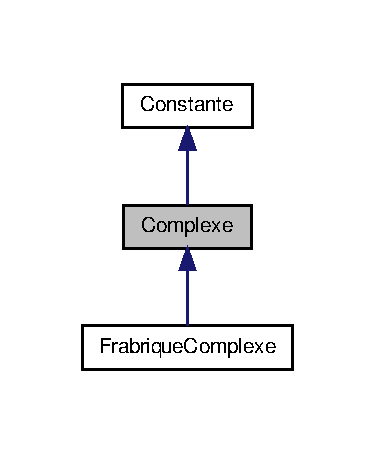
\includegraphics[width=142pt]{class_complexe__inherit__graph}
\end{center}
\end{figure}


\-Graphe de collaboration de \-Complexe\-:\nopagebreak
\begin{figure}[H]
\begin{center}
\leavevmode
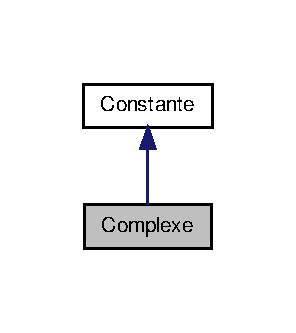
\includegraphics[width=142pt]{class_complexe__coll__graph}
\end{center}
\end{figure}
\subsection*{\-Fonctions membres publiques}
\begin{DoxyCompactItemize}
\item 
\hyperlink{class_complexe_af2cec56db6fdf59ed5ec761ffd4e1608}{\-Complexe} ()
\item 
\hyperlink{class_complexe_ae19286bc2c8f360e3fbc0d65526564d3}{\-Complexe} (\hyperlink{class_constante}{\-Constante} $\ast$r, \hyperlink{class_constante}{\-Constante} $\ast$i)
\item 
virtual \hyperlink{class_complexe_ac92996231047d39d40e11384bb9311b6}{$\sim$\-Complexe} ()
\item 
virtual \-Q\-String \hyperlink{class_complexe_a5141b5b092f78c06f60013e911ba4440}{afficher} () const 
\item 
\hyperlink{class_constante}{\-Constante} $\ast$ \hyperlink{class_complexe_a4441d56fc9776ce78efd8b5d95d9170b}{get\-Partie\-Reelle} () const 
\item 
\hyperlink{class_constante}{\-Constante} $\ast$ \hyperlink{class_complexe_a9e3e38b5362dd83812da9235594d1fcc}{get\-Partie\-Imaginaire} () const 
\item 
void \hyperlink{class_complexe_a7e57ea7cf760e132c80a148e2c344cce}{set\-Reelle} (\hyperlink{class_constante}{\-Constante} $\ast$re)
\item 
void \hyperlink{class_complexe_a2335ce4c53e2b11d4fa4bcbef45415ba}{set\-Imaginaire} (\hyperlink{class_constante}{\-Constante} $\ast$im)
\item 
\hyperlink{class_complexe_ac00d0b5ba1dea7d67c43d257e48fd7b5}{\-Complexe} (\hyperlink{class_constante}{\-Constante} $\ast$c)
\item 
bool \hyperlink{class_complexe_a64fbf7a898e40d86cc0fb2be00c4bddf}{reel\-\_\-pur} () const 
\item 
virtual \hyperlink{class_constante}{\-Constante} $\ast$ \hyperlink{class_complexe_adb3491a51a6b76d8e2c41ab87e519003}{addition} (\hyperlink{class_constante}{\-Constante} $\ast$c)
\item 
virtual \hyperlink{class_constante}{\-Constante} $\ast$ \hyperlink{class_complexe_a921d9d4a3efcf108cb437b265cd65c10}{produit} (\hyperlink{class_constante}{\-Constante} $\ast$c)
\item 
virtual \hyperlink{class_constante}{\-Constante} $\ast$ \hyperlink{class_complexe_a1a2f7b85999d542ebff0a9c0d082c1c8}{division} (\hyperlink{class_constante}{\-Constante} $\ast$c)
\item 
virtual \hyperlink{class_constante}{\-Constante} $\ast$ \hyperlink{class_complexe_a97bb77958c4012ed113c54f895f91e85}{signe} ()
\item 
virtual \hyperlink{class_constante}{\-Constante} $\ast$ \hyperlink{class_complexe_a07d706446560190792339549752f9ea3}{soustraction} (\hyperlink{class_constante}{\-Constante} $\ast$c)
\item 
virtual \hyperlink{class_constante}{\-Constante} $\ast$ \hyperlink{class_complexe_afb48ef33e0289c8f05a959f83d9ec621}{inv} ()
\item 
virtual \hyperlink{class_constante}{\-Constante} $\ast$ \hyperlink{class_complexe_a0b0532339249783cee39f28670bb7504}{fact} ()
\item 
virtual \hyperlink{class_constante}{\-Constante} $\ast$ \hyperlink{class_complexe_a58574399ad50181f94c8f167916b9db9}{sinus} (bool angle)
\item 
virtual \hyperlink{class_constante}{\-Constante} $\ast$ \hyperlink{class_complexe_a5b659cad17efee687fb8a889aef5da09}{cosinus} (bool angle)
\item 
virtual \hyperlink{class_constante}{\-Constante} $\ast$ \hyperlink{class_complexe_a221161f63e9176b49eb74de70ef73d78}{sinush} (bool angle)
\item 
virtual \hyperlink{class_constante}{\-Constante} $\ast$ \hyperlink{class_complexe_a356e44404acabb3e6bd8228f746fc3f5}{cosinush} (bool angle)
\item 
virtual \hyperlink{class_constante}{\-Constante} $\ast$ \hyperlink{class_complexe_a7602a9b9ca6e17445207b3632ceba643}{tangente} (bool angle)
\item 
virtual \hyperlink{class_constante}{\-Constante} $\ast$ \hyperlink{class_complexe_a649a2ad523bfe715950e2e0f3b28213d}{tangenteh} (bool angle)
\item 
virtual \hyperlink{class_constante}{\-Constante} $\ast$ \hyperlink{class_complexe_a8adb5d883810b1fdbcfa230f32100408}{log\-N} ()
\item 
virtual \hyperlink{class_constante}{\-Constante} $\ast$ \hyperlink{class_complexe_ada2cd39fae72dcf78fac8b361072b4e1}{log1} ()
\item 
virtual \hyperlink{class_constante}{\-Constante} $\ast$ \hyperlink{class_complexe_aaebd8e53e61cdea5504fc8f9fa5d2523}{puissance} (\hyperlink{class_constante}{\-Constante} $\ast$c)
\item 
virtual \hyperlink{class_constante}{\-Constante} $\ast$ \hyperlink{class_complexe_a7bbaa8c8695253acb93eb91eb1bd51c0}{carre} ()
\item 
virtual \hyperlink{class_constante}{\-Constante} $\ast$ \hyperlink{class_complexe_a7026e226db2bb64a1ca5c014fa8b6f43}{cube} ()
\item 
virtual \hyperlink{class_constante}{\-Constante} $\ast$ \hyperlink{class_complexe_ab7d41a46e8467b819afa76f658a12c01}{racine} ()
\end{DoxyCompactItemize}


\subsection{\-Description détaillée}


\-Définition à la ligne 20 du fichier complexe.\-h.



\subsection{\-Documentation des constructeurs et destructeur}
\hypertarget{class_complexe_af2cec56db6fdf59ed5ec761ffd4e1608}{\index{\-Complexe@{\-Complexe}!\-Complexe@{\-Complexe}}
\index{\-Complexe@{\-Complexe}!Complexe@{\-Complexe}}
\subsubsection[{\-Complexe}]{\setlength{\rightskip}{0pt plus 5cm}{\bf \-Complexe\-::\-Complexe} (
\begin{DoxyParamCaption}
{}
\end{DoxyParamCaption}
)\hspace{0.3cm}{\ttfamily  \mbox{[}inline\mbox{]}}}}\label{class_complexe_af2cec56db6fdf59ed5ec761ffd4e1608}


\-Définition à la ligne 26 du fichier complexe.\-h.



\-Voici le graphe des appelants de cette fonction \-:\nopagebreak
\begin{figure}[H]
\begin{center}
\leavevmode
\includegraphics[width=350pt]{class_complexe_af2cec56db6fdf59ed5ec761ffd4e1608_icgraph}
\end{center}
\end{figure}


\hypertarget{class_complexe_ae19286bc2c8f360e3fbc0d65526564d3}{\index{\-Complexe@{\-Complexe}!\-Complexe@{\-Complexe}}
\index{\-Complexe@{\-Complexe}!Complexe@{\-Complexe}}
\subsubsection[{\-Complexe}]{\setlength{\rightskip}{0pt plus 5cm}{\bf \-Complexe\-::\-Complexe} (
\begin{DoxyParamCaption}
\item[{{\bf \-Constante} $\ast$}]{r, }
\item[{{\bf \-Constante} $\ast$}]{i}
\end{DoxyParamCaption}
)}}\label{class_complexe_ae19286bc2c8f360e3fbc0d65526564d3}
\-Constructeur surchargé de complexe

\-On vérifie le type des 2 constantes, et on lève une exception si ce sont des complexes, car un complexe ne peut pas être composé lui même de complexes 
\begin{DoxyParams}{\-Paramètres}
{\em r} & la partie réelle est une \hyperlink{class_constante}{\-Constante} \\
\hline
{\em i} & la partie imaginaire est une \hyperlink{class_constante}{\-Constante} aussi\\
\hline
\end{DoxyParams}


\-Définition à la ligne 17 du fichier complexe.\-cpp.



\-Voici le graphe d'appel pour cette fonction \-:\nopagebreak
\begin{figure}[H]
\begin{center}
\leavevmode
\includegraphics[width=350pt]{class_complexe_ae19286bc2c8f360e3fbc0d65526564d3_cgraph}
\end{center}
\end{figure}


\hypertarget{class_complexe_ac92996231047d39d40e11384bb9311b6}{\index{\-Complexe@{\-Complexe}!$\sim$\-Complexe@{$\sim$\-Complexe}}
\index{$\sim$\-Complexe@{$\sim$\-Complexe}!Complexe@{\-Complexe}}
\subsubsection[{$\sim$\-Complexe}]{\setlength{\rightskip}{0pt plus 5cm}{\bf \-Complexe\-::$\sim$\-Complexe} (
\begin{DoxyParamCaption}
{}
\end{DoxyParamCaption}
)\hspace{0.3cm}{\ttfamily  \mbox{[}virtual\mbox{]}}}}\label{class_complexe_ac92996231047d39d40e11384bb9311b6}
\-Destructeru de complexe

\-Rétabli le dernier état annulé de la pile \-Historique.

\-Définition à la ligne 8 du fichier complexe.\-cpp.

\hypertarget{class_complexe_ac00d0b5ba1dea7d67c43d257e48fd7b5}{\index{\-Complexe@{\-Complexe}!\-Complexe@{\-Complexe}}
\index{\-Complexe@{\-Complexe}!Complexe@{\-Complexe}}
\subsubsection[{\-Complexe}]{\setlength{\rightskip}{0pt plus 5cm}{\bf \-Complexe\-::\-Complexe} (
\begin{DoxyParamCaption}
\item[{{\bf \-Constante} $\ast$}]{c}
\end{DoxyParamCaption}
)}}\label{class_complexe_ac00d0b5ba1dea7d67c43d257e48fd7b5}
\-Constructeur surchargé à un paramètre

\-On vérifie les types, et on crée un complexe qui n'aura qu'une partie réelle 
\begin{DoxyParams}{\-Paramètres}
{\em c} & seul paramètre, qui est une \hyperlink{class_constante}{\-Constante}\\
\hline
\end{DoxyParams}


\-Définition à la ligne 34 du fichier complexe.\-cpp.



\-Voici le graphe d'appel pour cette fonction \-:\nopagebreak
\begin{figure}[H]
\begin{center}
\leavevmode
\includegraphics[width=350pt]{class_complexe_ac00d0b5ba1dea7d67c43d257e48fd7b5_cgraph}
\end{center}
\end{figure}




\subsection{\-Documentation des fonctions membres}
\hypertarget{class_complexe_adb3491a51a6b76d8e2c41ab87e519003}{\index{\-Complexe@{\-Complexe}!addition@{addition}}
\index{addition@{addition}!Complexe@{\-Complexe}}
\subsubsection[{addition}]{\setlength{\rightskip}{0pt plus 5cm}{\bf \-Constante} $\ast$ {\bf \-Complexe\-::addition} (
\begin{DoxyParamCaption}
\item[{{\bf \-Constante} $\ast$}]{c}
\end{DoxyParamCaption}
)\hspace{0.3cm}{\ttfamily  \mbox{[}virtual\mbox{]}}}}\label{class_complexe_adb3491a51a6b76d8e2c41ab87e519003}
\-Addition de 2 complexes

\-On crée 3 complexes \-: {\itshape c\-\_\-entier\/}, construit à partir du paramètre, {\itshape re\/}, qui est l'addition des 2 parties réelles et {\itshape im\/}, qui est l'addition des 2 parties imaginaires \begin{DoxyReturn}{\-Renvoie}
\-Une {\itshape \hyperlink{class_constante}{\-Constante}\/}, qui est en fait un {\itshape \hyperlink{class_complexe}{\-Complexe}\/}, dont la partie imaginaire est {\itshape re\/} et la partie imaginaire {\itshape im\/}.
\end{DoxyReturn}


\-Réimplémentée à partir de \hyperlink{class_constante_a243b6eabd1fd476af827c5b523cddfac}{\-Constante}.



\-Définition à la ligne 73 du fichier complexe.\-cpp.



\-Voici le graphe d'appel pour cette fonction \-:\nopagebreak
\begin{figure}[H]
\begin{center}
\leavevmode
\includegraphics[width=350pt]{class_complexe_adb3491a51a6b76d8e2c41ab87e519003_cgraph}
\end{center}
\end{figure}




\-Voici le graphe des appelants de cette fonction \-:\nopagebreak
\begin{figure}[H]
\begin{center}
\leavevmode
\includegraphics[width=350pt]{class_complexe_adb3491a51a6b76d8e2c41ab87e519003_icgraph}
\end{center}
\end{figure}


\hypertarget{class_complexe_a5141b5b092f78c06f60013e911ba4440}{\index{\-Complexe@{\-Complexe}!afficher@{afficher}}
\index{afficher@{afficher}!Complexe@{\-Complexe}}
\subsubsection[{afficher}]{\setlength{\rightskip}{0pt plus 5cm}\-Q\-String {\bf \-Complexe\-::afficher} (
\begin{DoxyParamCaption}
{}
\end{DoxyParamCaption}
) const\hspace{0.3cm}{\ttfamily  \mbox{[}virtual\mbox{]}}}}\label{class_complexe_a5141b5b092f78c06f60013e911ba4440}
\-Méthode d'affichae d'un \hyperlink{class_complexe}{\-Complexe}

\-On vérifie le type de la partie imaginaire, et on crée une nouvelle constante de ce type. \-Si la partie imaginaire est nule, on affiche la partie réelle, sinon on affiche la partie réelle, un \$ et la partie imaginaire. \begin{DoxyReturn}{\-Renvoie}
\-Une {\itshape \-Q\-String\/} permettant l'affichage
\end{DoxyReturn}


\-Implémente \hyperlink{class_constante_a78b5d9ee6a7e70349db6641a08f77479}{\-Constante}.



\-Définition à la ligne 59 du fichier complexe.\-cpp.



\-Voici le graphe d'appel pour cette fonction \-:\nopagebreak
\begin{figure}[H]
\begin{center}
\leavevmode
\includegraphics[width=350pt]{class_complexe_a5141b5b092f78c06f60013e911ba4440_cgraph}
\end{center}
\end{figure}


\hypertarget{class_complexe_a7bbaa8c8695253acb93eb91eb1bd51c0}{\index{\-Complexe@{\-Complexe}!carre@{carre}}
\index{carre@{carre}!Complexe@{\-Complexe}}
\subsubsection[{carre}]{\setlength{\rightskip}{0pt plus 5cm}{\bf \-Constante} $\ast$ {\bf \-Complexe\-::carre} (
\begin{DoxyParamCaption}
{}
\end{DoxyParamCaption}
)\hspace{0.3cm}{\ttfamily  \mbox{[}virtual\mbox{]}}}}\label{class_complexe_a7bbaa8c8695253acb93eb91eb1bd51c0}


\-Réimplémentée à partir de \hyperlink{class_constante_af8029cf3c52e8fdadeb21647ee9591f3}{\-Constante}.



\-Définition à la ligne 204 du fichier complexe.\-cpp.



\-Voici le graphe d'appel pour cette fonction \-:\nopagebreak
\begin{figure}[H]
\begin{center}
\leavevmode
\includegraphics[width=350pt]{class_complexe_a7bbaa8c8695253acb93eb91eb1bd51c0_cgraph}
\end{center}
\end{figure}




\-Voici le graphe des appelants de cette fonction \-:\nopagebreak
\begin{figure}[H]
\begin{center}
\leavevmode
\includegraphics[width=350pt]{class_complexe_a7bbaa8c8695253acb93eb91eb1bd51c0_icgraph}
\end{center}
\end{figure}


\hypertarget{class_complexe_a5b659cad17efee687fb8a889aef5da09}{\index{\-Complexe@{\-Complexe}!cosinus@{cosinus}}
\index{cosinus@{cosinus}!Complexe@{\-Complexe}}
\subsubsection[{cosinus}]{\setlength{\rightskip}{0pt plus 5cm}{\bf \-Constante} $\ast$ {\bf \-Complexe\-::cosinus} (
\begin{DoxyParamCaption}
\item[{bool}]{angle}
\end{DoxyParamCaption}
)\hspace{0.3cm}{\ttfamily  \mbox{[}virtual\mbox{]}}}}\label{class_complexe_a5b659cad17efee687fb8a889aef5da09}


\-Réimplémentée à partir de \hyperlink{class_constante_af6784ed749b7f2be92d6017628e5b935}{\-Constante}.



\-Définition à la ligne 155 du fichier complexe.\-cpp.



\-Voici le graphe d'appel pour cette fonction \-:\nopagebreak
\begin{figure}[H]
\begin{center}
\leavevmode
\includegraphics[width=350pt]{class_complexe_a5b659cad17efee687fb8a889aef5da09_cgraph}
\end{center}
\end{figure}


\hypertarget{class_complexe_a356e44404acabb3e6bd8228f746fc3f5}{\index{\-Complexe@{\-Complexe}!cosinush@{cosinush}}
\index{cosinush@{cosinush}!Complexe@{\-Complexe}}
\subsubsection[{cosinush}]{\setlength{\rightskip}{0pt plus 5cm}{\bf \-Constante} $\ast$ {\bf \-Complexe\-::cosinush} (
\begin{DoxyParamCaption}
\item[{bool}]{angle}
\end{DoxyParamCaption}
)\hspace{0.3cm}{\ttfamily  \mbox{[}virtual\mbox{]}}}}\label{class_complexe_a356e44404acabb3e6bd8228f746fc3f5}


\-Réimplémentée à partir de \hyperlink{class_constante_a0b1cbba53e1112aa65a081ae6231acb5}{\-Constante}.



\-Définition à la ligne 171 du fichier complexe.\-cpp.



\-Voici le graphe d'appel pour cette fonction \-:\nopagebreak
\begin{figure}[H]
\begin{center}
\leavevmode
\includegraphics[width=350pt]{class_complexe_a356e44404acabb3e6bd8228f746fc3f5_cgraph}
\end{center}
\end{figure}


\hypertarget{class_complexe_a7026e226db2bb64a1ca5c014fa8b6f43}{\index{\-Complexe@{\-Complexe}!cube@{cube}}
\index{cube@{cube}!Complexe@{\-Complexe}}
\subsubsection[{cube}]{\setlength{\rightskip}{0pt plus 5cm}{\bf \-Constante} $\ast$ {\bf \-Complexe\-::cube} (
\begin{DoxyParamCaption}
{}
\end{DoxyParamCaption}
)\hspace{0.3cm}{\ttfamily  \mbox{[}virtual\mbox{]}}}}\label{class_complexe_a7026e226db2bb64a1ca5c014fa8b6f43}


\-Réimplémentée à partir de \hyperlink{class_constante_a4590414eecfb9e739194a321a73c7931}{\-Constante}.



\-Définition à la ligne 210 du fichier complexe.\-cpp.



\-Voici le graphe d'appel pour cette fonction \-:\nopagebreak
\begin{figure}[H]
\begin{center}
\leavevmode
\includegraphics[width=350pt]{class_complexe_a7026e226db2bb64a1ca5c014fa8b6f43_cgraph}
\end{center}
\end{figure}


\hypertarget{class_complexe_a1a2f7b85999d542ebff0a9c0d082c1c8}{\index{\-Complexe@{\-Complexe}!division@{division}}
\index{division@{division}!Complexe@{\-Complexe}}
\subsubsection[{division}]{\setlength{\rightskip}{0pt plus 5cm}{\bf \-Constante} $\ast$ {\bf \-Complexe\-::division} (
\begin{DoxyParamCaption}
\item[{{\bf \-Constante} $\ast$}]{c}
\end{DoxyParamCaption}
)\hspace{0.3cm}{\ttfamily  \mbox{[}virtual\mbox{]}}}}\label{class_complexe_a1a2f7b85999d542ebff0a9c0d082c1c8}
\-Division de 2 complexes

\-On utilise la multiplication par le conjugué du diviseur au numérateur et au dénominateur a+ib / c+id = (a+ib)$\ast$(c-\/id) / (c+id)$\ast$(c-\/id) = ... = \mbox{[}(ac+bd)/(c²+d²)\mbox{]} + i\mbox{[}(cb-\/ad)/(c²+d²)\mbox{]} \begin{DoxyReturn}{\-Renvoie}
\-Un {\itshape \hyperlink{class_complexe}{\-Complexe}\/} comme pour les autres opérations
\end{DoxyReturn}


\-Réimplémentée à partir de \hyperlink{class_constante_ac41fa56ac5ebdfbcc886b8d249fb876d}{\-Constante}.



\-Définition à la ligne 103 du fichier complexe.\-cpp.



\-Voici le graphe d'appel pour cette fonction \-:\nopagebreak
\begin{figure}[H]
\begin{center}
\leavevmode
\includegraphics[width=350pt]{class_complexe_a1a2f7b85999d542ebff0a9c0d082c1c8_cgraph}
\end{center}
\end{figure}




\-Voici le graphe des appelants de cette fonction \-:\nopagebreak
\begin{figure}[H]
\begin{center}
\leavevmode
\includegraphics[width=350pt]{class_complexe_a1a2f7b85999d542ebff0a9c0d082c1c8_icgraph}
\end{center}
\end{figure}


\hypertarget{class_complexe_a0b0532339249783cee39f28670bb7504}{\index{\-Complexe@{\-Complexe}!fact@{fact}}
\index{fact@{fact}!Complexe@{\-Complexe}}
\subsubsection[{fact}]{\setlength{\rightskip}{0pt plus 5cm}{\bf \-Constante} $\ast$ {\bf \-Complexe\-::fact} (
\begin{DoxyParamCaption}
{}
\end{DoxyParamCaption}
)\hspace{0.3cm}{\ttfamily  \mbox{[}virtual\mbox{]}}}}\label{class_complexe_a0b0532339249783cee39f28670bb7504}


\-Réimplémentée à partir de \hyperlink{class_constante_a96e23d33bd45f79589f8911473ef2e32}{\-Constante}.



\-Définition à la ligne 139 du fichier complexe.\-cpp.



\-Voici le graphe d'appel pour cette fonction \-:\nopagebreak
\begin{figure}[H]
\begin{center}
\leavevmode
\includegraphics[width=350pt]{class_complexe_a0b0532339249783cee39f28670bb7504_cgraph}
\end{center}
\end{figure}


\hypertarget{class_complexe_a9e3e38b5362dd83812da9235594d1fcc}{\index{\-Complexe@{\-Complexe}!get\-Partie\-Imaginaire@{get\-Partie\-Imaginaire}}
\index{get\-Partie\-Imaginaire@{get\-Partie\-Imaginaire}!Complexe@{\-Complexe}}
\subsubsection[{get\-Partie\-Imaginaire}]{\setlength{\rightskip}{0pt plus 5cm}{\bf \-Constante}$\ast$ {\bf \-Complexe\-::get\-Partie\-Imaginaire} (
\begin{DoxyParamCaption}
{}
\end{DoxyParamCaption}
) const\hspace{0.3cm}{\ttfamily  \mbox{[}inline\mbox{]}}}}\label{class_complexe_a9e3e38b5362dd83812da9235594d1fcc}


\-Définition à la ligne 31 du fichier complexe.\-h.



\-Voici le graphe des appelants de cette fonction \-:\nopagebreak
\begin{figure}[H]
\begin{center}
\leavevmode
\includegraphics[width=350pt]{class_complexe_a9e3e38b5362dd83812da9235594d1fcc_icgraph}
\end{center}
\end{figure}


\hypertarget{class_complexe_a4441d56fc9776ce78efd8b5d95d9170b}{\index{\-Complexe@{\-Complexe}!get\-Partie\-Reelle@{get\-Partie\-Reelle}}
\index{get\-Partie\-Reelle@{get\-Partie\-Reelle}!Complexe@{\-Complexe}}
\subsubsection[{get\-Partie\-Reelle}]{\setlength{\rightskip}{0pt plus 5cm}{\bf \-Constante}$\ast$ {\bf \-Complexe\-::get\-Partie\-Reelle} (
\begin{DoxyParamCaption}
{}
\end{DoxyParamCaption}
) const\hspace{0.3cm}{\ttfamily  \mbox{[}inline\mbox{]}}}}\label{class_complexe_a4441d56fc9776ce78efd8b5d95d9170b}


\-Définition à la ligne 30 du fichier complexe.\-h.



\-Voici le graphe des appelants de cette fonction \-:\nopagebreak
\begin{figure}[H]
\begin{center}
\leavevmode
\includegraphics[width=350pt]{class_complexe_a4441d56fc9776ce78efd8b5d95d9170b_icgraph}
\end{center}
\end{figure}


\hypertarget{class_complexe_afb48ef33e0289c8f05a959f83d9ec621}{\index{\-Complexe@{\-Complexe}!inv@{inv}}
\index{inv@{inv}!Complexe@{\-Complexe}}
\subsubsection[{inv}]{\setlength{\rightskip}{0pt plus 5cm}{\bf \-Constante} $\ast$ {\bf \-Complexe\-::inv} (
\begin{DoxyParamCaption}
{}
\end{DoxyParamCaption}
)\hspace{0.3cm}{\ttfamily  \mbox{[}virtual\mbox{]}}}}\label{class_complexe_afb48ef33e0289c8f05a959f83d9ec621}


\-Réimplémentée à partir de \hyperlink{class_constante_a5ea6dd472ce568576961fa78b3b674b5}{\-Constante}.



\-Définition à la ligne 196 du fichier complexe.\-cpp.



\-Voici le graphe d'appel pour cette fonction \-:\nopagebreak
\begin{figure}[H]
\begin{center}
\leavevmode
\includegraphics[width=350pt]{class_complexe_afb48ef33e0289c8f05a959f83d9ec621_cgraph}
\end{center}
\end{figure}




\-Voici le graphe des appelants de cette fonction \-:\nopagebreak
\begin{figure}[H]
\begin{center}
\leavevmode
\includegraphics[width=350pt]{class_complexe_afb48ef33e0289c8f05a959f83d9ec621_icgraph}
\end{center}
\end{figure}


\hypertarget{class_complexe_ada2cd39fae72dcf78fac8b361072b4e1}{\index{\-Complexe@{\-Complexe}!log1@{log1}}
\index{log1@{log1}!Complexe@{\-Complexe}}
\subsubsection[{log1}]{\setlength{\rightskip}{0pt plus 5cm}{\bf \-Constante} $\ast$ {\bf \-Complexe\-::log1} (
\begin{DoxyParamCaption}
{}
\end{DoxyParamCaption}
)\hspace{0.3cm}{\ttfamily  \mbox{[}virtual\mbox{]}}}}\label{class_complexe_ada2cd39fae72dcf78fac8b361072b4e1}


\-Réimplémentée à partir de \hyperlink{class_constante_aad178503c937682acd3c9f19aec37dc6}{\-Constante}.



\-Définition à la ligne 240 du fichier complexe.\-cpp.



\-Voici le graphe d'appel pour cette fonction \-:\nopagebreak
\begin{figure}[H]
\begin{center}
\leavevmode
\includegraphics[width=350pt]{class_complexe_ada2cd39fae72dcf78fac8b361072b4e1_cgraph}
\end{center}
\end{figure}


\hypertarget{class_complexe_a8adb5d883810b1fdbcfa230f32100408}{\index{\-Complexe@{\-Complexe}!log\-N@{log\-N}}
\index{log\-N@{log\-N}!Complexe@{\-Complexe}}
\subsubsection[{log\-N}]{\setlength{\rightskip}{0pt plus 5cm}{\bf \-Constante} $\ast$ {\bf \-Complexe\-::log\-N} (
\begin{DoxyParamCaption}
{}
\end{DoxyParamCaption}
)\hspace{0.3cm}{\ttfamily  \mbox{[}virtual\mbox{]}}}}\label{class_complexe_a8adb5d883810b1fdbcfa230f32100408}


\-Réimplémentée à partir de \hyperlink{class_constante_aa28e3269159806101c2ac0d09c036c2c}{\-Constante}.



\-Définition à la ligne 232 du fichier complexe.\-cpp.



\-Voici le graphe d'appel pour cette fonction \-:\nopagebreak
\begin{figure}[H]
\begin{center}
\leavevmode
\includegraphics[width=350pt]{class_complexe_a8adb5d883810b1fdbcfa230f32100408_cgraph}
\end{center}
\end{figure}


\hypertarget{class_complexe_a921d9d4a3efcf108cb437b265cd65c10}{\index{\-Complexe@{\-Complexe}!produit@{produit}}
\index{produit@{produit}!Complexe@{\-Complexe}}
\subsubsection[{produit}]{\setlength{\rightskip}{0pt plus 5cm}{\bf \-Constante} $\ast$ {\bf \-Complexe\-::produit} (
\begin{DoxyParamCaption}
\item[{{\bf \-Constante} $\ast$}]{c}
\end{DoxyParamCaption}
)\hspace{0.3cm}{\ttfamily  \mbox{[}virtual\mbox{]}}}}\label{class_complexe_a921d9d4a3efcf108cb437b265cd65c10}
\-Produit de 2 complexes

\-Comme pour l'addition, on crée trois complexes. \-Cette fois, {\itshape re\/} est le produit des parties réelles, de la forme a$\ast$c -\/ b$\ast$d, et {\itshape im\/} est le produit des parties imaginaires, de la forme a$\ast$d + c$\ast$b. \begin{DoxyReturn}{\-Renvoie}
\-Un {\itshape \hyperlink{class_complexe}{\-Complexe}\/} comme pour l'addition
\end{DoxyReturn}


\-Réimplémentée à partir de \hyperlink{class_constante_a650e88b74d2f8a052e6a11363b3ec816}{\-Constante}.



\-Définition à la ligne 88 du fichier complexe.\-cpp.



\-Voici le graphe d'appel pour cette fonction \-:\nopagebreak
\begin{figure}[H]
\begin{center}
\leavevmode
\includegraphics[width=350pt]{class_complexe_a921d9d4a3efcf108cb437b265cd65c10_cgraph}
\end{center}
\end{figure}




\-Voici le graphe des appelants de cette fonction \-:\nopagebreak
\begin{figure}[H]
\begin{center}
\leavevmode
\includegraphics[width=350pt]{class_complexe_a921d9d4a3efcf108cb437b265cd65c10_icgraph}
\end{center}
\end{figure}


\hypertarget{class_complexe_aaebd8e53e61cdea5504fc8f9fa5d2523}{\index{\-Complexe@{\-Complexe}!puissance@{puissance}}
\index{puissance@{puissance}!Complexe@{\-Complexe}}
\subsubsection[{puissance}]{\setlength{\rightskip}{0pt plus 5cm}{\bf \-Constante} $\ast$ {\bf \-Complexe\-::puissance} (
\begin{DoxyParamCaption}
\item[{{\bf \-Constante} $\ast$}]{c}
\end{DoxyParamCaption}
)\hspace{0.3cm}{\ttfamily  \mbox{[}virtual\mbox{]}}}}\label{class_complexe_aaebd8e53e61cdea5504fc8f9fa5d2523}


\-Réimplémentée à partir de \hyperlink{class_constante_a2ed5e0a77fb7766fbce6abb4ebd0b01e}{\-Constante}.



\-Définition à la ligne 224 du fichier complexe.\-cpp.



\-Voici le graphe d'appel pour cette fonction \-:\nopagebreak
\begin{figure}[H]
\begin{center}
\leavevmode
\includegraphics[width=350pt]{class_complexe_aaebd8e53e61cdea5504fc8f9fa5d2523_cgraph}
\end{center}
\end{figure}


\hypertarget{class_complexe_ab7d41a46e8467b819afa76f658a12c01}{\index{\-Complexe@{\-Complexe}!racine@{racine}}
\index{racine@{racine}!Complexe@{\-Complexe}}
\subsubsection[{racine}]{\setlength{\rightskip}{0pt plus 5cm}{\bf \-Constante} $\ast$ {\bf \-Complexe\-::racine} (
\begin{DoxyParamCaption}
{}
\end{DoxyParamCaption}
)\hspace{0.3cm}{\ttfamily  \mbox{[}virtual\mbox{]}}}}\label{class_complexe_ab7d41a46e8467b819afa76f658a12c01}


\-Réimplémentée à partir de \hyperlink{class_constante_a57604347a44e29f6aa7e36a045b4df1c}{\-Constante}.



\-Définition à la ligne 216 du fichier complexe.\-cpp.



\-Voici le graphe d'appel pour cette fonction \-:\nopagebreak
\begin{figure}[H]
\begin{center}
\leavevmode
\includegraphics[width=350pt]{class_complexe_ab7d41a46e8467b819afa76f658a12c01_cgraph}
\end{center}
\end{figure}


\hypertarget{class_complexe_a64fbf7a898e40d86cc0fb2be00c4bddf}{\index{\-Complexe@{\-Complexe}!reel\-\_\-pur@{reel\-\_\-pur}}
\index{reel\-\_\-pur@{reel\-\_\-pur}!Complexe@{\-Complexe}}
\subsubsection[{reel\-\_\-pur}]{\setlength{\rightskip}{0pt plus 5cm}bool {\bf \-Complexe\-::reel\-\_\-pur} (
\begin{DoxyParamCaption}
{}
\end{DoxyParamCaption}
) const}}\label{class_complexe_a64fbf7a898e40d86cc0fb2be00c4bddf}


\-Définition à la ligne 248 du fichier complexe.\-cpp.



\-Voici le graphe d'appel pour cette fonction \-:\nopagebreak
\begin{figure}[H]
\begin{center}
\leavevmode
\includegraphics[width=350pt]{class_complexe_a64fbf7a898e40d86cc0fb2be00c4bddf_cgraph}
\end{center}
\end{figure}




\-Voici le graphe des appelants de cette fonction \-:\nopagebreak
\begin{figure}[H]
\begin{center}
\leavevmode
\includegraphics[width=350pt]{class_complexe_a64fbf7a898e40d86cc0fb2be00c4bddf_icgraph}
\end{center}
\end{figure}


\hypertarget{class_complexe_a2335ce4c53e2b11d4fa4bcbef45415ba}{\index{\-Complexe@{\-Complexe}!set\-Imaginaire@{set\-Imaginaire}}
\index{set\-Imaginaire@{set\-Imaginaire}!Complexe@{\-Complexe}}
\subsubsection[{set\-Imaginaire}]{\setlength{\rightskip}{0pt plus 5cm}void {\bf \-Complexe\-::set\-Imaginaire} (
\begin{DoxyParamCaption}
\item[{{\bf \-Constante} $\ast$}]{im}
\end{DoxyParamCaption}
)\hspace{0.3cm}{\ttfamily  \mbox{[}inline\mbox{]}}}}\label{class_complexe_a2335ce4c53e2b11d4fa4bcbef45415ba}


\-Définition à la ligne 33 du fichier complexe.\-h.



\-Voici le graphe des appelants de cette fonction \-:\nopagebreak
\begin{figure}[H]
\begin{center}
\leavevmode
\includegraphics[width=350pt]{class_complexe_a2335ce4c53e2b11d4fa4bcbef45415ba_icgraph}
\end{center}
\end{figure}


\hypertarget{class_complexe_a7e57ea7cf760e132c80a148e2c344cce}{\index{\-Complexe@{\-Complexe}!set\-Reelle@{set\-Reelle}}
\index{set\-Reelle@{set\-Reelle}!Complexe@{\-Complexe}}
\subsubsection[{set\-Reelle}]{\setlength{\rightskip}{0pt plus 5cm}void {\bf \-Complexe\-::set\-Reelle} (
\begin{DoxyParamCaption}
\item[{{\bf \-Constante} $\ast$}]{re}
\end{DoxyParamCaption}
)\hspace{0.3cm}{\ttfamily  \mbox{[}inline\mbox{]}}}}\label{class_complexe_a7e57ea7cf760e132c80a148e2c344cce}


\-Définition à la ligne 32 du fichier complexe.\-h.



\-Voici le graphe des appelants de cette fonction \-:\nopagebreak
\begin{figure}[H]
\begin{center}
\leavevmode
\includegraphics[width=350pt]{class_complexe_a7e57ea7cf760e132c80a148e2c344cce_icgraph}
\end{center}
\end{figure}


\hypertarget{class_complexe_a97bb77958c4012ed113c54f895f91e85}{\index{\-Complexe@{\-Complexe}!signe@{signe}}
\index{signe@{signe}!Complexe@{\-Complexe}}
\subsubsection[{signe}]{\setlength{\rightskip}{0pt plus 5cm}{\bf \-Constante} $\ast$ {\bf \-Complexe\-::signe} (
\begin{DoxyParamCaption}
{}
\end{DoxyParamCaption}
)\hspace{0.3cm}{\ttfamily  \mbox{[}virtual\mbox{]}}}}\label{class_complexe_a97bb77958c4012ed113c54f895f91e85}
\-Changement de signe

\-On recopie tout d'abord la constante, qu'on caste ensuite en complexe. \-On crée un entier de valeur -\/1 qu'on va multiplier avec les parties réelles et imaginaires de 2 nouveaux complexes qui servent temporairement pour ensuite modifier la valeur du complexe initial \begin{DoxyReturn}{\-Renvoie}
\-Le nouveau {\itshape \hyperlink{class_complexe}{\-Complexe}\/} 
\end{DoxyReturn}


\-Réimplémentée à partir de \hyperlink{class_constante_a59fcc22949ea02eb02244dad693696aa}{\-Constante}.



\-Définition à la ligne 115 du fichier complexe.\-cpp.



\-Voici le graphe d'appel pour cette fonction \-:\nopagebreak
\begin{figure}[H]
\begin{center}
\leavevmode
\includegraphics[width=350pt]{class_complexe_a97bb77958c4012ed113c54f895f91e85_cgraph}
\end{center}
\end{figure}




\-Voici le graphe des appelants de cette fonction \-:\nopagebreak
\begin{figure}[H]
\begin{center}
\leavevmode
\includegraphics[width=350pt]{class_complexe_a97bb77958c4012ed113c54f895f91e85_icgraph}
\end{center}
\end{figure}


\hypertarget{class_complexe_a58574399ad50181f94c8f167916b9db9}{\index{\-Complexe@{\-Complexe}!sinus@{sinus}}
\index{sinus@{sinus}!Complexe@{\-Complexe}}
\subsubsection[{sinus}]{\setlength{\rightskip}{0pt plus 5cm}{\bf \-Constante} $\ast$ {\bf \-Complexe\-::sinus} (
\begin{DoxyParamCaption}
\item[{bool}]{angle}
\end{DoxyParamCaption}
)\hspace{0.3cm}{\ttfamily  \mbox{[}virtual\mbox{]}}}}\label{class_complexe_a58574399ad50181f94c8f167916b9db9}


\-Réimplémentée à partir de \hyperlink{class_constante_a3b6827eba7936c4ce61f64da9dd826b4}{\-Constante}.



\-Définition à la ligne 147 du fichier complexe.\-cpp.



\-Voici le graphe d'appel pour cette fonction \-:\nopagebreak
\begin{figure}[H]
\begin{center}
\leavevmode
\includegraphics[width=350pt]{class_complexe_a58574399ad50181f94c8f167916b9db9_cgraph}
\end{center}
\end{figure}


\hypertarget{class_complexe_a221161f63e9176b49eb74de70ef73d78}{\index{\-Complexe@{\-Complexe}!sinush@{sinush}}
\index{sinush@{sinush}!Complexe@{\-Complexe}}
\subsubsection[{sinush}]{\setlength{\rightskip}{0pt plus 5cm}{\bf \-Constante} $\ast$ {\bf \-Complexe\-::sinush} (
\begin{DoxyParamCaption}
\item[{bool}]{angle}
\end{DoxyParamCaption}
)\hspace{0.3cm}{\ttfamily  \mbox{[}virtual\mbox{]}}}}\label{class_complexe_a221161f63e9176b49eb74de70ef73d78}


\-Réimplémentée à partir de \hyperlink{class_constante_a101b4506f71295a23c764d34b7f7ecfb}{\-Constante}.



\-Définition à la ligne 163 du fichier complexe.\-cpp.



\-Voici le graphe d'appel pour cette fonction \-:\nopagebreak
\begin{figure}[H]
\begin{center}
\leavevmode
\includegraphics[width=350pt]{class_complexe_a221161f63e9176b49eb74de70ef73d78_cgraph}
\end{center}
\end{figure}


\hypertarget{class_complexe_a07d706446560190792339549752f9ea3}{\index{\-Complexe@{\-Complexe}!soustraction@{soustraction}}
\index{soustraction@{soustraction}!Complexe@{\-Complexe}}
\subsubsection[{soustraction}]{\setlength{\rightskip}{0pt plus 5cm}{\bf \-Constante} $\ast$ {\bf \-Complexe\-::soustraction} (
\begin{DoxyParamCaption}
\item[{{\bf \-Constante} $\ast$}]{c}
\end{DoxyParamCaption}
)\hspace{0.3cm}{\ttfamily  \mbox{[}virtual\mbox{]}}}}\label{class_complexe_a07d706446560190792339549752f9ea3}
\-Différence de deux complexes

\-De la même façon, cette fois {\itshape re\/} va être la différence des 2 parties réelles, et {\itshape im\/} la différence des parties imaginaires. \begin{DoxyReturn}{\-Renvoie}
\-Un {\itshape \hyperlink{class_complexe}{\-Complexe}\/} dont la partie réelle est {\itshape re\/} et la partie imaginaire est {\itshape im\/}.
\end{DoxyReturn}


\-Réimplémentée à partir de \hyperlink{class_constante_a3f3e5ad91d9e4eef33a5e6955fe91cb5}{\-Constante}.



\-Définition à la ligne 127 du fichier complexe.\-cpp.



\-Voici le graphe d'appel pour cette fonction \-:\nopagebreak
\begin{figure}[H]
\begin{center}
\leavevmode
\includegraphics[width=350pt]{class_complexe_a07d706446560190792339549752f9ea3_cgraph}
\end{center}
\end{figure}




\-Voici le graphe des appelants de cette fonction \-:\nopagebreak
\begin{figure}[H]
\begin{center}
\leavevmode
\includegraphics[width=350pt]{class_complexe_a07d706446560190792339549752f9ea3_icgraph}
\end{center}
\end{figure}


\hypertarget{class_complexe_a7602a9b9ca6e17445207b3632ceba643}{\index{\-Complexe@{\-Complexe}!tangente@{tangente}}
\index{tangente@{tangente}!Complexe@{\-Complexe}}
\subsubsection[{tangente}]{\setlength{\rightskip}{0pt plus 5cm}{\bf \-Constante} $\ast$ {\bf \-Complexe\-::tangente} (
\begin{DoxyParamCaption}
\item[{bool}]{angle}
\end{DoxyParamCaption}
)\hspace{0.3cm}{\ttfamily  \mbox{[}virtual\mbox{]}}}}\label{class_complexe_a7602a9b9ca6e17445207b3632ceba643}


\-Réimplémentée à partir de \hyperlink{class_constante_a51bffad2fa33a397de6ed422a621b1a1}{\-Constante}.



\-Définition à la ligne 179 du fichier complexe.\-cpp.



\-Voici le graphe d'appel pour cette fonction \-:\nopagebreak
\begin{figure}[H]
\begin{center}
\leavevmode
\includegraphics[width=350pt]{class_complexe_a7602a9b9ca6e17445207b3632ceba643_cgraph}
\end{center}
\end{figure}


\hypertarget{class_complexe_a649a2ad523bfe715950e2e0f3b28213d}{\index{\-Complexe@{\-Complexe}!tangenteh@{tangenteh}}
\index{tangenteh@{tangenteh}!Complexe@{\-Complexe}}
\subsubsection[{tangenteh}]{\setlength{\rightskip}{0pt plus 5cm}{\bf \-Constante} $\ast$ {\bf \-Complexe\-::tangenteh} (
\begin{DoxyParamCaption}
\item[{bool}]{angle}
\end{DoxyParamCaption}
)\hspace{0.3cm}{\ttfamily  \mbox{[}virtual\mbox{]}}}}\label{class_complexe_a649a2ad523bfe715950e2e0f3b28213d}


\-Réimplémentée à partir de \hyperlink{class_constante_a6f5f971e61ac831355f1182289c3952f}{\-Constante}.



\-Définition à la ligne 187 du fichier complexe.\-cpp.



\-Voici le graphe d'appel pour cette fonction \-:\nopagebreak
\begin{figure}[H]
\begin{center}
\leavevmode
\includegraphics[width=350pt]{class_complexe_a649a2ad523bfe715950e2e0f3b28213d_cgraph}
\end{center}
\end{figure}




\-La documentation de cette classe a été générée à partir des fichiers suivants \-:\begin{DoxyCompactItemize}
\item 
/home/yuntux/\-U\-T\-C/\-G\-I02/\-L\-O21/projet/projet\-\_\-propre/\hyperlink{complexe_8h}{complexe.\-h}\item 
/home/yuntux/\-U\-T\-C/\-G\-I02/\-L\-O21/projet/projet\-\_\-propre/\hyperlink{complexe_8cpp}{complexe.\-cpp}\end{DoxyCompactItemize}

\hypertarget{class_constante}{\section{\-Constante \-Class \-Reference}
\label{class_constante}\index{\-Constante@{\-Constante}}
}


\-Inheritance diagram for \-Constante\-:
\nopagebreak
\begin{figure}[H]
\begin{center}
\leavevmode
\includegraphics[width=350pt]{class_constante__inherit__graph}
\end{center}
\end{figure}
\subsection*{\-Public \-Member \-Functions}
\begin{DoxyCompactItemize}
\item 
\hypertarget{class_constante_a78b5d9ee6a7e70349db6641a08f77479}{virtual \-Q\-String {\bfseries afficher} () const =0}\label{class_constante_a78b5d9ee6a7e70349db6641a08f77479}

\item 
\hypertarget{class_constante_a580f4535e16d4c9331da85750be6e5ad}{virtual \hyperlink{class_constante}{\-Constante} $\ast$ {\bfseries addition} (\hyperlink{class_constante}{\-Constante} $\ast$c)=0}\label{class_constante_a580f4535e16d4c9331da85750be6e5ad}

\item 
\hypertarget{class_constante_ad805854dd4e53f0ef5b2d482398b682a}{virtual \hyperlink{class_constante}{\-Constante} $\ast$ {\bfseries produit} (\hyperlink{class_constante}{\-Constante} $\ast$c)=0}\label{class_constante_ad805854dd4e53f0ef5b2d482398b682a}

\item 
\hypertarget{class_constante_ab9b969ad6ad0d8463d44a1273667ee79}{virtual \hyperlink{class_constante}{\-Constante} $\ast$ {\bfseries division} (\hyperlink{class_constante}{\-Constante} $\ast$c)=0}\label{class_constante_ab9b969ad6ad0d8463d44a1273667ee79}

\item 
\hypertarget{class_constante_a1c6f79dbc7623529ee4fd5ae9c556b45}{virtual \hyperlink{class_constante}{\-Constante} $\ast$ {\bfseries signe} ()=0}\label{class_constante_a1c6f79dbc7623529ee4fd5ae9c556b45}

\item 
\hypertarget{class_constante_ac6fb071229429f82cf489f8313461efa}{\hyperlink{class_constante}{\-Constante} $\ast$ {\bfseries recopie} ()}\label{class_constante_ac6fb071229429f82cf489f8313461efa}

\item 
\hypertarget{class_constante_ad1df4970f093fdb4235d4945ec2dbf12}{virtual \hyperlink{class_constante}{\-Constante} $\ast$ {\bfseries soustraction} (\hyperlink{class_constante}{\-Constante} $\ast$c)=0}\label{class_constante_ad1df4970f093fdb4235d4945ec2dbf12}

\item 
\hypertarget{class_constante_a63d03e59594b74aa2fbc35f559b0ad46}{virtual \hyperlink{class_constante}{\-Constante} $\ast$ {\bfseries inv} ()=0}\label{class_constante_a63d03e59594b74aa2fbc35f559b0ad46}

\item 
\hypertarget{class_constante_a57dafd18c718935af9f97dcbb8de9ad9}{virtual \hyperlink{class_constante}{\-Constante} $\ast$ {\bfseries fact} ()=0}\label{class_constante_a57dafd18c718935af9f97dcbb8de9ad9}

\item 
\hypertarget{class_constante_ad1a0ed2f6f6e9c3e7fc3f0c4ffaeaa76}{virtual \hyperlink{class_constante}{\-Constante} $\ast$ {\bfseries sinus} ()=0}\label{class_constante_ad1a0ed2f6f6e9c3e7fc3f0c4ffaeaa76}

\end{DoxyCompactItemize}


\-The documentation for this class was generated from the following files\-:\begin{DoxyCompactItemize}
\item 
/home/yuntux/\-U\-T\-C/\-G\-I02/\-L\-O21/projet/lo21-\/npi.\-2/\hyperlink{constante_8h}{constante.\-h}\item 
/home/yuntux/\-U\-T\-C/\-G\-I02/\-L\-O21/projet/lo21-\/npi.\-2/constante.\-cpp\end{DoxyCompactItemize}

\hypertarget{class_entier}{\section{\-Référence de la classe \-Entier}
\label{class_entier}\index{\-Entier@{\-Entier}}
}


{\ttfamily \#include $<$entier.\-h$>$}



\-Graphe d'héritage de \-Entier\-:\nopagebreak
\begin{figure}[H]
\begin{center}
\leavevmode
\includegraphics[width=142pt]{class_entier__inherit__graph}
\end{center}
\end{figure}


\-Graphe de collaboration de \-Entier\-:\nopagebreak
\begin{figure}[H]
\begin{center}
\leavevmode
\includegraphics[width=142pt]{class_entier__coll__graph}
\end{center}
\end{figure}
\subsection*{\-Fonctions membres publiques}
\begin{DoxyCompactItemize}
\item 
\hyperlink{class_entier_a35115c0f47f2d94e1697e20624a1c4d1}{\-Entier} (int e)
\item 
\hyperlink{class_entier_a94158ae6fbad4c9a74815716f5f0f629}{\-Entier} (\hyperlink{class_constante}{\-Constante} $\ast$c)
\item 
virtual \hyperlink{class_entier_ab44549f9d4abf2fd4425f8e3374cdc08}{$\sim$\-Entier} ()
\item 
virtual \-Q\-String \hyperlink{class_entier_adc0a7554faa45a68eb7432798b6892cc}{afficher} () const 
\item 
int \hyperlink{class_entier_afe38ee7f81afc3c88a2c774ff0af2bcd}{get\-Valeur} () const 
\item 
void \hyperlink{class_entier_a22e1c5d0ecf304cd6033e6bf453cc0c1}{set\-Valeur} (int v)
\item 
virtual \hyperlink{class_constante}{\-Constante} $\ast$ \hyperlink{class_entier_ab093dd3f0aa7777c4300362f7ba78ff4}{addition} (\hyperlink{class_constante}{\-Constante} $\ast$c)
\item 
virtual \hyperlink{class_constante}{\-Constante} $\ast$ \hyperlink{class_entier_aa83349a1b984adbd53766ebac2614faf}{produit} (\hyperlink{class_constante}{\-Constante} $\ast$c)
\item 
virtual \hyperlink{class_constante}{\-Constante} $\ast$ \hyperlink{class_entier_a36ce54a35fc9ab69bef2cffebee01c69}{signe} ()
\item 
virtual \hyperlink{class_constante}{\-Constante} $\ast$ \hyperlink{class_entier_afc338f1f177942411a3c8e0e19fce6ce}{division} (\hyperlink{class_constante}{\-Constante} $\ast$c)
\item 
virtual \hyperlink{class_constante}{\-Constante} $\ast$ \hyperlink{class_entier_a880936c128f077144cd266199cd27585}{soustraction} (\hyperlink{class_constante}{\-Constante} $\ast$c)
\item 
int \hyperlink{class_entier_a29ebe7b4a2b8e8135736389977339330}{mod} (\hyperlink{class_entier}{\-Entier} $\ast$c)
\item 
virtual \hyperlink{class_constante}{\-Constante} $\ast$ \hyperlink{class_entier_a094c16293e7853eafa646d1613db3034}{fact} ()
\item 
virtual \hyperlink{class_constante}{\-Constante} $\ast$ \hyperlink{class_entier_a5e4a3ab5cc280d0e082300207712d5d8}{inv} ()
\item 
virtual \hyperlink{class_constante}{\-Constante} $\ast$ \hyperlink{class_entier_a1c4613f03f0c7818d1a092714b9077bd}{sinus} (bool angle)
\item 
virtual \hyperlink{class_constante}{\-Constante} $\ast$ \hyperlink{class_entier_a77e37975ae8575ac9a41d4e41688429a}{cosinus} (bool angle)
\item 
virtual \hyperlink{class_constante}{\-Constante} $\ast$ \hyperlink{class_entier_a1b87da533d3a1a7c75c327526f3492c0}{sinush} (bool angle)
\item 
virtual \hyperlink{class_constante}{\-Constante} $\ast$ \hyperlink{class_entier_ae7fbbe73ca85a3bad129d2285f7485aa}{cosinush} (bool angle)
\item 
virtual \hyperlink{class_constante}{\-Constante} $\ast$ \hyperlink{class_entier_ae07a386db45cb20dddbb3dc8738a4115}{tangente} (bool angle)
\item 
virtual \hyperlink{class_constante}{\-Constante} $\ast$ \hyperlink{class_entier_aa8d0a9958c7f7eaf38c60922e2716601}{tangenteh} (bool angle)
\item 
virtual \hyperlink{class_constante}{\-Constante} $\ast$ \hyperlink{class_entier_a4bc40041f47a027ef00d3e71869fdaf9}{log\-N} ()
\item 
virtual \hyperlink{class_constante}{\-Constante} $\ast$ \hyperlink{class_entier_abe28b3a25a9b179d36c35c7081638ab3}{log1} ()
\item 
virtual \hyperlink{class_constante}{\-Constante} $\ast$ \hyperlink{class_entier_ae789623eeda06e02ba54c14dab64c399}{puissance} (\hyperlink{class_constante}{\-Constante} $\ast$c)
\item 
virtual \hyperlink{class_constante}{\-Constante} $\ast$ \hyperlink{class_entier_ac93c2be5a977a38c560ee01eae5b9381}{carre} ()
\item 
virtual \hyperlink{class_constante}{\-Constante} $\ast$ \hyperlink{class_entier_ac4aa9142ca284291935f5e2880c3b612}{cube} ()
\item 
virtual \hyperlink{class_constante}{\-Constante} $\ast$ \hyperlink{class_entier_ae5459f97866c5240e8a1417f425b5a05}{racine} ()
\end{DoxyCompactItemize}


\subsection{\-Description détaillée}


\-Définition à la ligne 18 du fichier entier.\-h.



\subsection{\-Documentation des constructeurs et destructeur}
\hypertarget{class_entier_a35115c0f47f2d94e1697e20624a1c4d1}{\index{\-Entier@{\-Entier}!\-Entier@{\-Entier}}
\index{\-Entier@{\-Entier}!Entier@{\-Entier}}
\subsubsection[{\-Entier}]{\setlength{\rightskip}{0pt plus 5cm}{\bf \-Entier\-::\-Entier} (
\begin{DoxyParamCaption}
\item[{int}]{e}
\end{DoxyParamCaption}
)\hspace{0.3cm}{\ttfamily  \mbox{[}inline\mbox{]}}}}\label{class_entier_a35115c0f47f2d94e1697e20624a1c4d1}


\-Définition à la ligne 22 du fichier entier.\-h.



\-Voici le graphe des appelants de cette fonction \-:\nopagebreak
\begin{figure}[H]
\begin{center}
\leavevmode
\includegraphics[width=350pt]{class_entier_a35115c0f47f2d94e1697e20624a1c4d1_icgraph}
\end{center}
\end{figure}


\hypertarget{class_entier_a94158ae6fbad4c9a74815716f5f0f629}{\index{\-Entier@{\-Entier}!\-Entier@{\-Entier}}
\index{\-Entier@{\-Entier}!Entier@{\-Entier}}
\subsubsection[{\-Entier}]{\setlength{\rightskip}{0pt plus 5cm}{\bf \-Entier\-::\-Entier} (
\begin{DoxyParamCaption}
\item[{{\bf \-Constante} $\ast$}]{c}
\end{DoxyParamCaption}
)}}\label{class_entier_a94158ae6fbad4c9a74815716f5f0f629}
\-Constructeur d'entier

\-On vérifie le type de la constante passée en paramètre, et si c'est un entier, on recopie sa valeur dans le nouvel entier, sinon on lève une exception. 
\begin{DoxyParams}{\-Paramètres}
{\em c} & \-Une constante, donc entier, réel, rationnel ou complexe\\
\hline
\end{DoxyParams}


\-Définition à la ligne 9 du fichier entier.\-cpp.



\-Voici le graphe d'appel pour cette fonction \-:\nopagebreak
\begin{figure}[H]
\begin{center}
\leavevmode
\includegraphics[width=350pt]{class_entier_a94158ae6fbad4c9a74815716f5f0f629_cgraph}
\end{center}
\end{figure}


\hypertarget{class_entier_ab44549f9d4abf2fd4425f8e3374cdc08}{\index{\-Entier@{\-Entier}!$\sim$\-Entier@{$\sim$\-Entier}}
\index{$\sim$\-Entier@{$\sim$\-Entier}!Entier@{\-Entier}}
\subsubsection[{$\sim$\-Entier}]{\setlength{\rightskip}{0pt plus 5cm}virtual {\bf \-Entier\-::$\sim$\-Entier} (
\begin{DoxyParamCaption}
{}
\end{DoxyParamCaption}
)\hspace{0.3cm}{\ttfamily  \mbox{[}inline, virtual\mbox{]}}}}\label{class_entier_ab44549f9d4abf2fd4425f8e3374cdc08}


\-Définition à la ligne 24 du fichier entier.\-h.



\subsection{\-Documentation des fonctions membres}
\hypertarget{class_entier_ab093dd3f0aa7777c4300362f7ba78ff4}{\index{\-Entier@{\-Entier}!addition@{addition}}
\index{addition@{addition}!Entier@{\-Entier}}
\subsubsection[{addition}]{\setlength{\rightskip}{0pt plus 5cm}{\bf \-Constante} $\ast$ {\bf \-Entier\-::addition} (
\begin{DoxyParamCaption}
\item[{{\bf \-Constante} $\ast$}]{c}
\end{DoxyParamCaption}
)\hspace{0.3cm}{\ttfamily  \mbox{[}virtual\mbox{]}}}}\label{class_entier_ab093dd3f0aa7777c4300362f7ba78ff4}
\-Somme de 2 entiers

\-On vérifie le type du paramètre, et on crée une nouvelle instance de ce type en fonction, dont le ou les attributs seront en fait la somme des 2 entiers dont l'on veut calculer l'addition.\-Cependant, si on est en mode \hyperlink{class_entier}{\-Entier}, on ne doit pas avoir les autres types de constante. 
\begin{DoxyParams}{\-Paramètres}
{\em c} & \-Une constante \\
\hline
\end{DoxyParams}
\begin{DoxyReturn}{\-Renvoie}
\-Un {\itshape \hyperlink{class_entier}{\-Entier}\/} construit, car on utilisera toujours les formes complexes pour les calculs
\end{DoxyReturn}


\-Réimplémentée à partir de \hyperlink{class_constante_a243b6eabd1fd476af827c5b523cddfac}{\-Constante}.



\-Définition à la ligne 40 du fichier entier.\-cpp.



\-Voici le graphe d'appel pour cette fonction \-:\nopagebreak
\begin{figure}[H]
\begin{center}
\leavevmode
\includegraphics[width=350pt]{class_entier_ab093dd3f0aa7777c4300362f7ba78ff4_cgraph}
\end{center}
\end{figure}




\-Voici le graphe des appelants de cette fonction \-:\nopagebreak
\begin{figure}[H]
\begin{center}
\leavevmode
\includegraphics[width=350pt]{class_entier_ab093dd3f0aa7777c4300362f7ba78ff4_icgraph}
\end{center}
\end{figure}


\hypertarget{class_entier_adc0a7554faa45a68eb7432798b6892cc}{\index{\-Entier@{\-Entier}!afficher@{afficher}}
\index{afficher@{afficher}!Entier@{\-Entier}}
\subsubsection[{afficher}]{\setlength{\rightskip}{0pt plus 5cm}virtual \-Q\-String {\bf \-Entier\-::afficher} (
\begin{DoxyParamCaption}
{}
\end{DoxyParamCaption}
) const\hspace{0.3cm}{\ttfamily  \mbox{[}inline, virtual\mbox{]}}}}\label{class_entier_adc0a7554faa45a68eb7432798b6892cc}


\-Implémente \hyperlink{class_constante_a78b5d9ee6a7e70349db6641a08f77479}{\-Constante}.



\-Définition à la ligne 25 du fichier entier.\-h.

\hypertarget{class_entier_ac93c2be5a977a38c560ee01eae5b9381}{\index{\-Entier@{\-Entier}!carre@{carre}}
\index{carre@{carre}!Entier@{\-Entier}}
\subsubsection[{carre}]{\setlength{\rightskip}{0pt plus 5cm}{\bf \-Constante} $\ast$ {\bf \-Entier\-::carre} (
\begin{DoxyParamCaption}
{}
\end{DoxyParamCaption}
)\hspace{0.3cm}{\ttfamily  \mbox{[}virtual\mbox{]}}}}\label{class_entier_ac93c2be5a977a38c560ee01eae5b9381}
\-Fonction carré

\-On crée un nouvel \hyperlink{class_entier}{\-Entier} dont la valeur est le résultat du carré \begin{DoxyReturn}{\-Renvoie}
\-Un {\itshape \hyperlink{class_entier}{\-Entier}\/} construit construit à partir du résultat de la fonction
\end{DoxyReturn}


\-Réimplémentée à partir de \hyperlink{class_constante_af8029cf3c52e8fdadeb21647ee9591f3}{\-Constante}.



\-Définition à la ligne 293 du fichier entier.\-cpp.



\-Voici le graphe d'appel pour cette fonction \-:\nopagebreak
\begin{figure}[H]
\begin{center}
\leavevmode
\includegraphics[width=260pt]{class_entier_ac93c2be5a977a38c560ee01eae5b9381_cgraph}
\end{center}
\end{figure}


\hypertarget{class_entier_a77e37975ae8575ac9a41d4e41688429a}{\index{\-Entier@{\-Entier}!cosinus@{cosinus}}
\index{cosinus@{cosinus}!Entier@{\-Entier}}
\subsubsection[{cosinus}]{\setlength{\rightskip}{0pt plus 5cm}{\bf \-Constante} $\ast$ {\bf \-Entier\-::cosinus} (
\begin{DoxyParamCaption}
\item[{bool}]{angle}
\end{DoxyParamCaption}
)\hspace{0.3cm}{\ttfamily  \mbox{[}virtual\mbox{]}}}}\label{class_entier_a77e37975ae8575ac9a41d4e41688429a}
\-Calcul du \-Cosinus

\-Si le paramètre est vrai, on se situe en mode \-Degré. \-Dans ce cas, il faut multiplier la valeur par \-P\-I/180, car la fonction {\itshape cos\/} de cmath est définie en radians. 
\begin{DoxyParams}{\-Paramètres}
{\em angle} & \-Sert à savoir si l'on est en mode \-Degré ou non \\
\hline
\end{DoxyParams}
\begin{DoxyReturn}{\-Renvoie}
\-Un {\itshape \hyperlink{class_entier}{\-Entier}\/} construit construit à partir d'un entier contenant la valeur du cosinus
\end{DoxyReturn}


\-Réimplémentée à partir de \hyperlink{class_constante_af6784ed749b7f2be92d6017628e5b935}{\-Constante}.



\-Définition à la ligne 158 du fichier entier.\-cpp.



\-Voici le graphe d'appel pour cette fonction \-:\nopagebreak
\begin{figure}[H]
\begin{center}
\leavevmode
\includegraphics[width=272pt]{class_entier_a77e37975ae8575ac9a41d4e41688429a_cgraph}
\end{center}
\end{figure}


\hypertarget{class_entier_ae7fbbe73ca85a3bad129d2285f7485aa}{\index{\-Entier@{\-Entier}!cosinush@{cosinush}}
\index{cosinush@{cosinush}!Entier@{\-Entier}}
\subsubsection[{cosinush}]{\setlength{\rightskip}{0pt plus 5cm}{\bf \-Constante} $\ast$ {\bf \-Entier\-::cosinush} (
\begin{DoxyParamCaption}
\item[{bool}]{angle}
\end{DoxyParamCaption}
)\hspace{0.3cm}{\ttfamily  \mbox{[}virtual\mbox{]}}}}\label{class_entier_ae7fbbe73ca85a3bad129d2285f7485aa}
\-Calcul du \-Cosinus \-Hyperbolique

\-Si le paramètre est vrai, on se situe en mode \-Degré. \-Dans ce cas, il faut multiplier la valeur par \-P\-I/180, car la fonction {\itshape cosh\/} de cmath est définie en radians. 
\begin{DoxyParams}{\-Paramètres}
{\em angle} & \-Sert à savoir si l'on est en mode \-Degré ou non \\
\hline
\end{DoxyParams}
\begin{DoxyReturn}{\-Renvoie}
\-Un {\itshape \hyperlink{class_entier}{\-Entier}\/} construit construit à partir d'un entier contenant la valeur du cosinus hyperbolique
\end{DoxyReturn}


\-Réimplémentée à partir de \hyperlink{class_constante_a0b1cbba53e1112aa65a081ae6231acb5}{\-Constante}.



\-Définition à la ligne 188 du fichier entier.\-cpp.



\-Voici le graphe d'appel pour cette fonction \-:\nopagebreak
\begin{figure}[H]
\begin{center}
\leavevmode
\includegraphics[width=278pt]{class_entier_ae7fbbe73ca85a3bad129d2285f7485aa_cgraph}
\end{center}
\end{figure}


\hypertarget{class_entier_ac4aa9142ca284291935f5e2880c3b612}{\index{\-Entier@{\-Entier}!cube@{cube}}
\index{cube@{cube}!Entier@{\-Entier}}
\subsubsection[{cube}]{\setlength{\rightskip}{0pt plus 5cm}{\bf \-Constante} $\ast$ {\bf \-Entier\-::cube} (
\begin{DoxyParamCaption}
{}
\end{DoxyParamCaption}
)\hspace{0.3cm}{\ttfamily  \mbox{[}virtual\mbox{]}}}}\label{class_entier_ac4aa9142ca284291935f5e2880c3b612}
\-Fonction cube

\-On crée un nouvel \hyperlink{class_entier}{\-Entier} dont la valeur est le résultat du cube \begin{DoxyReturn}{\-Renvoie}
\-Un {\itshape \hyperlink{class_entier}{\-Entier}\/} construit construit à partir du résultat de la fonction
\end{DoxyReturn}


\-Réimplémentée à partir de \hyperlink{class_constante_a4590414eecfb9e739194a321a73c7931}{\-Constante}.



\-Définition à la ligne 304 du fichier entier.\-cpp.



\-Voici le graphe d'appel pour cette fonction \-:\nopagebreak
\begin{figure}[H]
\begin{center}
\leavevmode
\includegraphics[width=260pt]{class_entier_ac4aa9142ca284291935f5e2880c3b612_cgraph}
\end{center}
\end{figure}


\hypertarget{class_entier_afc338f1f177942411a3c8e0e19fce6ce}{\index{\-Entier@{\-Entier}!division@{division}}
\index{division@{division}!Entier@{\-Entier}}
\subsubsection[{division}]{\setlength{\rightskip}{0pt plus 5cm}{\bf \-Constante} $\ast$ {\bf \-Entier\-::division} (
\begin{DoxyParamCaption}
\item[{{\bf \-Constante} $\ast$}]{c}
\end{DoxyParamCaption}
)\hspace{0.3cm}{\ttfamily  \mbox{[}virtual\mbox{]}}}}\label{class_entier_afc338f1f177942411a3c8e0e19fce6ce}
\-Division d'entiers

\-Comme pour la somme et le produit, on vérifie le type du paramètre, et on crée une nouvelle instance de ce type qui contiendra le quotient demandé. \-Cependant, normalement en mode \hyperlink{class_entier}{\-Entier}, on ne doit avoir que des entiers. 
\begin{DoxyParams}{\-Paramètres}
{\em c} & \-Une \hyperlink{class_constante}{\-Constante} \\
\hline
\end{DoxyParams}
\begin{DoxyReturn}{\-Renvoie}
\-Un {\itshape \hyperlink{class_entier}{\-Entier}\/} construit contenant le quotient
\end{DoxyReturn}


\-Réimplémentée à partir de \hyperlink{class_constante_ac41fa56ac5ebdfbcc886b8d249fb876d}{\-Constante}.



\-Définition à la ligne 93 du fichier entier.\-cpp.



\-Voici le graphe d'appel pour cette fonction \-:\nopagebreak
\begin{figure}[H]
\begin{center}
\leavevmode
\includegraphics[width=350pt]{class_entier_afc338f1f177942411a3c8e0e19fce6ce_cgraph}
\end{center}
\end{figure}


\hypertarget{class_entier_a094c16293e7853eafa646d1613db3034}{\index{\-Entier@{\-Entier}!fact@{fact}}
\index{fact@{fact}!Entier@{\-Entier}}
\subsubsection[{fact}]{\setlength{\rightskip}{0pt plus 5cm}{\bf \-Constante} $\ast$ {\bf \-Entier\-::fact} (
\begin{DoxyParamCaption}
{}
\end{DoxyParamCaption}
)\hspace{0.3cm}{\ttfamily  \mbox{[}virtual\mbox{]}}}}\label{class_entier_a094c16293e7853eafa646d1613db3034}
\-Calcul du factoriel

\-De manière itérative, le résultat est 1 si la valeur de l'entier est 0, et sinon on fait le calcul proprement dit \begin{DoxyReturn}{\-Renvoie}
\-Un nouveau {\itshape \hyperlink{class_complexe}{\-Complexe}\/}, construit à partir de l'entier qui contient la valeur du factoriel
\end{DoxyReturn}


\-Réimplémentée à partir de \hyperlink{class_constante_a96e23d33bd45f79589f8911473ef2e32}{\-Constante}.



\-Définition à la ligne 125 du fichier entier.\-cpp.



\-Voici le graphe d'appel pour cette fonction \-:\nopagebreak
\begin{figure}[H]
\begin{center}
\leavevmode
\includegraphics[width=272pt]{class_entier_a094c16293e7853eafa646d1613db3034_cgraph}
\end{center}
\end{figure}


\hypertarget{class_entier_afe38ee7f81afc3c88a2c774ff0af2bcd}{\index{\-Entier@{\-Entier}!get\-Valeur@{get\-Valeur}}
\index{get\-Valeur@{get\-Valeur}!Entier@{\-Entier}}
\subsubsection[{get\-Valeur}]{\setlength{\rightskip}{0pt plus 5cm}int {\bf \-Entier\-::get\-Valeur} (
\begin{DoxyParamCaption}
{}
\end{DoxyParamCaption}
) const\hspace{0.3cm}{\ttfamily  \mbox{[}inline\mbox{]}}}}\label{class_entier_afe38ee7f81afc3c88a2c774ff0af2bcd}


\-Définition à la ligne 26 du fichier entier.\-h.



\-Voici le graphe des appelants de cette fonction \-:\nopagebreak
\begin{figure}[H]
\begin{center}
\leavevmode
\includegraphics[width=350pt]{class_entier_afe38ee7f81afc3c88a2c774ff0af2bcd_icgraph}
\end{center}
\end{figure}


\hypertarget{class_entier_a5e4a3ab5cc280d0e082300207712d5d8}{\index{\-Entier@{\-Entier}!inv@{inv}}
\index{inv@{inv}!Entier@{\-Entier}}
\subsubsection[{inv}]{\setlength{\rightskip}{0pt plus 5cm}{\bf \-Constante} $\ast$ {\bf \-Entier\-::inv} (
\begin{DoxyParamCaption}
{}
\end{DoxyParamCaption}
)\hspace{0.3cm}{\ttfamily  \mbox{[}virtual\mbox{]}}}}\label{class_entier_a5e4a3ab5cc280d0e082300207712d5d8}
\-Inverse d'un entier

\-L'inverse d'un nombre est situé entre 0 et 1. \-Si l'on est en mode entier, on a une importante perte de précision, car on ne retournera que 0 ou 1 \begin{DoxyReturn}{\-Renvoie}
\-Un {\itshape \hyperlink{class_rationnel}{\-Rationnel}\/} car on perd moins de précisions comme cela
\end{DoxyReturn}


\-Réimplémentée à partir de \hyperlink{class_constante_a5ea6dd472ce568576961fa78b3b674b5}{\-Constante}.



\-Définition à la ligne 236 du fichier entier.\-cpp.



\-Voici le graphe d'appel pour cette fonction \-:\nopagebreak
\begin{figure}[H]
\begin{center}
\leavevmode
\includegraphics[width=268pt]{class_entier_a5e4a3ab5cc280d0e082300207712d5d8_cgraph}
\end{center}
\end{figure}


\hypertarget{class_entier_abe28b3a25a9b179d36c35c7081638ab3}{\index{\-Entier@{\-Entier}!log1@{log1}}
\index{log1@{log1}!Entier@{\-Entier}}
\subsubsection[{log1}]{\setlength{\rightskip}{0pt plus 5cm}{\bf \-Constante} $\ast$ {\bf \-Entier\-::log1} (
\begin{DoxyParamCaption}
{}
\end{DoxyParamCaption}
)\hspace{0.3cm}{\ttfamily  \mbox{[}virtual\mbox{]}}}}\label{class_entier_abe28b3a25a9b179d36c35c7081638ab3}
\-Logarithme décimal

\-On crée un nouvel \hyperlink{class_entier}{\-Entier} dont la valeur est celle du logarithme décimal de l'entier initial. \begin{DoxyReturn}{\-Renvoie}
\-Un {\itshape \hyperlink{class_entier}{\-Entier}\/} construit construit avec cet entier
\end{DoxyReturn}


\-Réimplémentée à partir de \hyperlink{class_constante_aad178503c937682acd3c9f19aec37dc6}{\-Constante}.



\-Définition à la ligne 259 du fichier entier.\-cpp.



\-Voici le graphe d'appel pour cette fonction \-:\nopagebreak
\begin{figure}[H]
\begin{center}
\leavevmode
\includegraphics[width=256pt]{class_entier_abe28b3a25a9b179d36c35c7081638ab3_cgraph}
\end{center}
\end{figure}


\hypertarget{class_entier_a4bc40041f47a027ef00d3e71869fdaf9}{\index{\-Entier@{\-Entier}!log\-N@{log\-N}}
\index{log\-N@{log\-N}!Entier@{\-Entier}}
\subsubsection[{log\-N}]{\setlength{\rightskip}{0pt plus 5cm}{\bf \-Constante} $\ast$ {\bf \-Entier\-::log\-N} (
\begin{DoxyParamCaption}
{}
\end{DoxyParamCaption}
)\hspace{0.3cm}{\ttfamily  \mbox{[}virtual\mbox{]}}}}\label{class_entier_a4bc40041f47a027ef00d3e71869fdaf9}
\-Logarithme népérien

\-On crée un nouvel \hyperlink{class_entier}{\-Entier} dont la valeur est celle du logarithme népérien de l'entier initial. \begin{DoxyReturn}{\-Renvoie}
\-Un {\itshape \hyperlink{class_entier}{\-Entier}\/} construit construit avec cet entier
\end{DoxyReturn}


\-Réimplémentée à partir de \hyperlink{class_constante_aa28e3269159806101c2ac0d09c036c2c}{\-Constante}.



\-Définition à la ligne 247 du fichier entier.\-cpp.



\-Voici le graphe d'appel pour cette fonction \-:\nopagebreak
\begin{figure}[H]
\begin{center}
\leavevmode
\includegraphics[width=258pt]{class_entier_a4bc40041f47a027ef00d3e71869fdaf9_cgraph}
\end{center}
\end{figure}


\hypertarget{class_entier_a29ebe7b4a2b8e8135736389977339330}{\index{\-Entier@{\-Entier}!mod@{mod}}
\index{mod@{mod}!Entier@{\-Entier}}
\subsubsection[{mod}]{\setlength{\rightskip}{0pt plus 5cm}int {\bf \-Entier\-::mod} (
\begin{DoxyParamCaption}
\item[{{\bf \-Entier} $\ast$}]{c}
\end{DoxyParamCaption}
)}}\label{class_entier_a29ebe7b4a2b8e8135736389977339330}
\hypertarget{class_entier_aa83349a1b984adbd53766ebac2614faf}{\index{\-Entier@{\-Entier}!produit@{produit}}
\index{produit@{produit}!Entier@{\-Entier}}
\subsubsection[{produit}]{\setlength{\rightskip}{0pt plus 5cm}{\bf \-Constante} $\ast$ {\bf \-Entier\-::produit} (
\begin{DoxyParamCaption}
\item[{{\bf \-Constante} $\ast$}]{c}
\end{DoxyParamCaption}
)\hspace{0.3cm}{\ttfamily  \mbox{[}virtual\mbox{]}}}}\label{class_entier_aa83349a1b984adbd53766ebac2614faf}
\-Produit de deux entiers

\-Comme pour la somme, on vérifie le type du paramètre, et on crée une nouvelle instance de ce type qui contiendra le produit demandé. \-Cependant, normalement en mode \hyperlink{class_entier}{\-Entier}, on ne doit avoir que des entiers. 
\begin{DoxyParams}{\-Paramètres}
{\em c} & \-Une \hyperlink{class_constante}{\-Constante} \\
\hline
\end{DoxyParams}
\begin{DoxyReturn}{\-Renvoie}
\-Un {\itshape \hyperlink{class_entier}{\-Entier}\/} construit contenant le produit
\end{DoxyReturn}


\-Réimplémentée à partir de \hyperlink{class_constante_a650e88b74d2f8a052e6a11363b3ec816}{\-Constante}.



\-Définition à la ligne 65 du fichier entier.\-cpp.



\-Voici le graphe d'appel pour cette fonction \-:\nopagebreak
\begin{figure}[H]
\begin{center}
\leavevmode
\includegraphics[width=350pt]{class_entier_aa83349a1b984adbd53766ebac2614faf_cgraph}
\end{center}
\end{figure}




\-Voici le graphe des appelants de cette fonction \-:\nopagebreak
\begin{figure}[H]
\begin{center}
\leavevmode
\includegraphics[width=276pt]{class_entier_aa83349a1b984adbd53766ebac2614faf_icgraph}
\end{center}
\end{figure}


\hypertarget{class_entier_ae789623eeda06e02ba54c14dab64c399}{\index{\-Entier@{\-Entier}!puissance@{puissance}}
\index{puissance@{puissance}!Entier@{\-Entier}}
\subsubsection[{puissance}]{\setlength{\rightskip}{0pt plus 5cm}{\bf \-Constante} $\ast$ {\bf \-Entier\-::puissance} (
\begin{DoxyParamCaption}
\item[{{\bf \-Constante} $\ast$}]{c}
\end{DoxyParamCaption}
)\hspace{0.3cm}{\ttfamily  \mbox{[}virtual\mbox{]}}}}\label{class_entier_ae789623eeda06e02ba54c14dab64c399}
\-Puissance de deux entiers

\-On effectue un transtypage en entier afin de récupérer l'exposant sous forme entière. \-On calcule ensuite grâce à la fonction {\itshape pow\/} de la bibliothèque {\itshape cmath\/}. 
\begin{DoxyParams}{\-Paramètres}
{\em c} & \-Une {\itshape \hyperlink{class_constante}{\-Constante}\/} qui sera l'exposant \\
\hline
\end{DoxyParams}
\begin{DoxyReturn}{\-Renvoie}
\-Un {\itshape \hyperlink{class_entier}{\-Entier}\/} construit construit à partir du résultat
\end{DoxyReturn}


\-Réimplémentée à partir de \hyperlink{class_constante_a2ed5e0a77fb7766fbce6abb4ebd0b01e}{\-Constante}.



\-Définition à la ligne 271 du fichier entier.\-cpp.



\-Voici le graphe d'appel pour cette fonction \-:\nopagebreak
\begin{figure}[H]
\begin{center}
\leavevmode
\includegraphics[width=298pt]{class_entier_ae789623eeda06e02ba54c14dab64c399_cgraph}
\end{center}
\end{figure}


\hypertarget{class_entier_ae5459f97866c5240e8a1417f425b5a05}{\index{\-Entier@{\-Entier}!racine@{racine}}
\index{racine@{racine}!Entier@{\-Entier}}
\subsubsection[{racine}]{\setlength{\rightskip}{0pt plus 5cm}{\bf \-Constante} $\ast$ {\bf \-Entier\-::racine} (
\begin{DoxyParamCaption}
{}
\end{DoxyParamCaption}
)\hspace{0.3cm}{\ttfamily  \mbox{[}virtual\mbox{]}}}}\label{class_entier_ae5459f97866c5240e8a1417f425b5a05}
\-Fonction racine carrée

\-On crée un nouvel \hyperlink{class_entier}{\-Entier} dont la valeur est le résultat de la racine carrée \begin{DoxyReturn}{\-Renvoie}
\-Un {\itshape \hyperlink{class_entier}{\-Entier}\/} construit construit à partir du résultat de la fonction
\end{DoxyReturn}


\-Réimplémentée à partir de \hyperlink{class_constante_a57604347a44e29f6aa7e36a045b4df1c}{\-Constante}.



\-Définition à la ligne 315 du fichier entier.\-cpp.



\-Voici le graphe d'appel pour cette fonction \-:\nopagebreak
\begin{figure}[H]
\begin{center}
\leavevmode
\includegraphics[width=264pt]{class_entier_ae5459f97866c5240e8a1417f425b5a05_cgraph}
\end{center}
\end{figure}


\hypertarget{class_entier_a22e1c5d0ecf304cd6033e6bf453cc0c1}{\index{\-Entier@{\-Entier}!set\-Valeur@{set\-Valeur}}
\index{set\-Valeur@{set\-Valeur}!Entier@{\-Entier}}
\subsubsection[{set\-Valeur}]{\setlength{\rightskip}{0pt plus 5cm}void {\bf \-Entier\-::set\-Valeur} (
\begin{DoxyParamCaption}
\item[{int}]{v}
\end{DoxyParamCaption}
)\hspace{0.3cm}{\ttfamily  \mbox{[}inline\mbox{]}}}}\label{class_entier_a22e1c5d0ecf304cd6033e6bf453cc0c1}


\-Définition à la ligne 27 du fichier entier.\-h.

\hypertarget{class_entier_a36ce54a35fc9ab69bef2cffebee01c69}{\index{\-Entier@{\-Entier}!signe@{signe}}
\index{signe@{signe}!Entier@{\-Entier}}
\subsubsection[{signe}]{\setlength{\rightskip}{0pt plus 5cm}{\bf \-Constante} $\ast$ {\bf \-Entier\-::signe} (
\begin{DoxyParamCaption}
{}
\end{DoxyParamCaption}
)\hspace{0.3cm}{\ttfamily  \mbox{[}virtual\mbox{]}}}}\label{class_entier_a36ce54a35fc9ab69bef2cffebee01c69}
\-Inversion de signe d'un entier

\-On crée un nouvel entier dont la valeur est l'opposée de celle initiale \begin{DoxyReturn}{\-Renvoie}
\-Un {\itshape \hyperlink{class_entier}{\-Entier}\/}, de valeur opposée
\end{DoxyReturn}


\-Réimplémentée à partir de \hyperlink{class_constante_a59fcc22949ea02eb02244dad693696aa}{\-Constante}.



\-Définition à la ligne 105 du fichier entier.\-cpp.



\-Voici le graphe d'appel pour cette fonction \-:\nopagebreak
\begin{figure}[H]
\begin{center}
\leavevmode
\includegraphics[width=262pt]{class_entier_a36ce54a35fc9ab69bef2cffebee01c69_cgraph}
\end{center}
\end{figure}


\hypertarget{class_entier_a1c4613f03f0c7818d1a092714b9077bd}{\index{\-Entier@{\-Entier}!sinus@{sinus}}
\index{sinus@{sinus}!Entier@{\-Entier}}
\subsubsection[{sinus}]{\setlength{\rightskip}{0pt plus 5cm}{\bf \-Constante} $\ast$ {\bf \-Entier\-::sinus} (
\begin{DoxyParamCaption}
\item[{bool}]{angle}
\end{DoxyParamCaption}
)\hspace{0.3cm}{\ttfamily  \mbox{[}virtual\mbox{]}}}}\label{class_entier_a1c4613f03f0c7818d1a092714b9077bd}
\-Calcul du \-Sinus

\-Si le paramètre est vrai, on se situe en mode \-Degré. \-Dans ce cas, il faut multiplier la valeur par \-P\-I/180, car la fonction {\itshape sin\/} de cmath est définie en radians. 
\begin{DoxyParams}{\-Paramètres}
{\em angle} & \-Sert à savoir si l'on est en mode \-Degré ou non \\
\hline
\end{DoxyParams}
\begin{DoxyReturn}{\-Renvoie}
\-Un {\itshape \hyperlink{class_entier}{\-Entier}\/} construit construit à partir d'un entier contenant la valeur du sinus
\end{DoxyReturn}


\-Réimplémentée à partir de \hyperlink{class_constante_a3b6827eba7936c4ce61f64da9dd826b4}{\-Constante}.



\-Définition à la ligne 143 du fichier entier.\-cpp.



\-Voici le graphe d'appel pour cette fonction \-:\nopagebreak
\begin{figure}[H]
\begin{center}
\leavevmode
\includegraphics[width=262pt]{class_entier_a1c4613f03f0c7818d1a092714b9077bd_cgraph}
\end{center}
\end{figure}


\hypertarget{class_entier_a1b87da533d3a1a7c75c327526f3492c0}{\index{\-Entier@{\-Entier}!sinush@{sinush}}
\index{sinush@{sinush}!Entier@{\-Entier}}
\subsubsection[{sinush}]{\setlength{\rightskip}{0pt plus 5cm}{\bf \-Constante} $\ast$ {\bf \-Entier\-::sinush} (
\begin{DoxyParamCaption}
\item[{bool}]{angle}
\end{DoxyParamCaption}
)\hspace{0.3cm}{\ttfamily  \mbox{[}virtual\mbox{]}}}}\label{class_entier_a1b87da533d3a1a7c75c327526f3492c0}
\-Calcul du \-Sinus \-Hyperbolique

\-Si le paramètre est vrai, on se situe en mode \-Degré. \-Dans ce cas, il faut multiplier la valeur par \-P\-I/180, car la fonction {\itshape sinh\/} de cmath est définie en radians. 
\begin{DoxyParams}{\-Paramètres}
{\em angle} & \-Sert à savoir si l'on est en mode \-Degré ou non \\
\hline
\end{DoxyParams}
\begin{DoxyReturn}{\-Renvoie}
\-Un {\itshape \hyperlink{class_entier}{\-Entier}\/} construit construit à partir d'un entier contenant la valeur du sinus hyperbolique
\end{DoxyReturn}


\-Réimplémentée à partir de \hyperlink{class_constante_a101b4506f71295a23c764d34b7f7ecfb}{\-Constante}.



\-Définition à la ligne 173 du fichier entier.\-cpp.



\-Voici le graphe d'appel pour cette fonction \-:\nopagebreak
\begin{figure}[H]
\begin{center}
\leavevmode
\includegraphics[width=268pt]{class_entier_a1b87da533d3a1a7c75c327526f3492c0_cgraph}
\end{center}
\end{figure}


\hypertarget{class_entier_a880936c128f077144cd266199cd27585}{\index{\-Entier@{\-Entier}!soustraction@{soustraction}}
\index{soustraction@{soustraction}!Entier@{\-Entier}}
\subsubsection[{soustraction}]{\setlength{\rightskip}{0pt plus 5cm}{\bf \-Constante} $\ast$ {\bf \-Entier\-::soustraction} (
\begin{DoxyParamCaption}
\item[{{\bf \-Constante} $\ast$}]{c}
\end{DoxyParamCaption}
)\hspace{0.3cm}{\ttfamily  \mbox{[}virtual\mbox{]}}}}\label{class_entier_a880936c128f077144cd266199cd27585}
\-Différence d'entiers

\-Comme pour les autres opérations, on vérifie le type du paramètre, et on crée une nouvelle instance de ce type qui contiendra la différence voulue. \-Cependant, normalement en mode \hyperlink{class_entier}{\-Entier}, on ne doit avoir que des entiers. 
\begin{DoxyParams}{\-Paramètres}
{\em c} & \-Une \hyperlink{class_constante}{\-Constante} \\
\hline
\end{DoxyParams}
\begin{DoxyReturn}{\-Renvoie}
\-Un {\itshape \hyperlink{class_entier}{\-Entier}\/} construit contenant la différence
\end{DoxyReturn}


\-Réimplémentée à partir de \hyperlink{class_constante_a3f3e5ad91d9e4eef33a5e6955fe91cb5}{\-Constante}.



\-Définition à la ligne 114 du fichier entier.\-cpp.



\-Voici le graphe d'appel pour cette fonction \-:\nopagebreak
\begin{figure}[H]
\begin{center}
\leavevmode
\includegraphics[width=350pt]{class_entier_a880936c128f077144cd266199cd27585_cgraph}
\end{center}
\end{figure}


\hypertarget{class_entier_ae07a386db45cb20dddbb3dc8738a4115}{\index{\-Entier@{\-Entier}!tangente@{tangente}}
\index{tangente@{tangente}!Entier@{\-Entier}}
\subsubsection[{tangente}]{\setlength{\rightskip}{0pt plus 5cm}{\bf \-Constante} $\ast$ {\bf \-Entier\-::tangente} (
\begin{DoxyParamCaption}
\item[{bool}]{angle}
\end{DoxyParamCaption}
)\hspace{0.3cm}{\ttfamily  \mbox{[}virtual\mbox{]}}}}\label{class_entier_ae07a386db45cb20dddbb3dc8738a4115}
\-Calcul de la \-Tangente

\-Si le paramètre est vrai, on se situe en mode \-Degré. \-Dans ce cas, il faut multiplier la valeur par \-P\-I/180, car la fonction {\itshape tan\/} de cmath est définie en radians. 
\begin{DoxyParams}{\-Paramètres}
{\em angle} & \-Sert à savoir si l'on est en mode \-Degré ou non \\
\hline
\end{DoxyParams}
\begin{DoxyReturn}{\-Renvoie}
\-Un {\itshape \hyperlink{class_entier}{\-Entier}\/} construit construit à partir d'un entier contenant la valeur de la tangente
\end{DoxyReturn}


\-Réimplémentée à partir de \hyperlink{class_constante_a51bffad2fa33a397de6ed422a621b1a1}{\-Constante}.



\-Définition à la ligne 204 du fichier entier.\-cpp.



\-Voici le graphe d'appel pour cette fonction \-:\nopagebreak
\begin{figure}[H]
\begin{center}
\leavevmode
\includegraphics[width=276pt]{class_entier_ae07a386db45cb20dddbb3dc8738a4115_cgraph}
\end{center}
\end{figure}


\hypertarget{class_entier_aa8d0a9958c7f7eaf38c60922e2716601}{\index{\-Entier@{\-Entier}!tangenteh@{tangenteh}}
\index{tangenteh@{tangenteh}!Entier@{\-Entier}}
\subsubsection[{tangenteh}]{\setlength{\rightskip}{0pt plus 5cm}{\bf \-Constante} $\ast$ {\bf \-Entier\-::tangenteh} (
\begin{DoxyParamCaption}
\item[{bool}]{angle}
\end{DoxyParamCaption}
)\hspace{0.3cm}{\ttfamily  \mbox{[}virtual\mbox{]}}}}\label{class_entier_aa8d0a9958c7f7eaf38c60922e2716601}
\-Calcul de la \-Tangente \-Hyperbolique

\-Si le paramètre est vrai, on se situe en mode \-Degré. \-Dans ce cas, il faut multiplier la valeur par \-P\-I/180, car la fonction {\itshape tanh\/} de cmath est définie en radians. 
\begin{DoxyParams}{\-Paramètres}
{\em angle} & \-Sert à savoir si l'on est en mode \-Degré ou non \\
\hline
\end{DoxyParams}
\begin{DoxyReturn}{\-Renvoie}
\-Un {\itshape \hyperlink{class_entier}{\-Entier}\/} construit construit à partir d'un entier contenant la valeur de la tangente hyperbolique
\end{DoxyReturn}


\-Réimplémentée à partir de \hyperlink{class_constante_a6f5f971e61ac831355f1182289c3952f}{\-Constante}.



\-Définition à la ligne 220 du fichier entier.\-cpp.



\-Voici le graphe d'appel pour cette fonction \-:\nopagebreak
\begin{figure}[H]
\begin{center}
\leavevmode
\includegraphics[width=282pt]{class_entier_aa8d0a9958c7f7eaf38c60922e2716601_cgraph}
\end{center}
\end{figure}




\-La documentation de cette classe a été générée à partir des fichiers suivants \-:\begin{DoxyCompactItemize}
\item 
/home/yuntux/\-U\-T\-C/\-G\-I02/\-L\-O21/projet/projet\-\_\-propre/\hyperlink{entier_8h}{entier.\-h}\item 
/home/yuntux/\-U\-T\-C/\-G\-I02/\-L\-O21/projet/projet\-\_\-propre/\hyperlink{entier_8cpp}{entier.\-cpp}\end{DoxyCompactItemize}

\hypertarget{class_expression}{\section{\-Référence de la classe \-Expression}
\label{class_expression}\index{\-Expression@{\-Expression}}
}


{\ttfamily \#include $<$expression.\-h$>$}



\-Graphe d'héritage de \-Expression\-:\nopagebreak
\begin{figure}[H]
\begin{center}
\leavevmode
\includegraphics[width=144pt]{class_expression__inherit__graph}
\end{center}
\end{figure}


\-Graphe de collaboration de \-Expression\-:\nopagebreak
\begin{figure}[H]
\begin{center}
\leavevmode
\includegraphics[width=144pt]{class_expression__coll__graph}
\end{center}
\end{figure}
\subsection*{\-Fonctions membres publiques}
\begin{DoxyCompactItemize}
\item 
\hyperlink{class_expression_ac25fb301ae3947c964a4da9a95883e72}{\-Expression} (\-Q\-String s)
\item 
virtual \hyperlink{class_expression_a2f6cee3469dea6cbc3e5af93587f7c25}{$\sim$\-Expression} ()
\item 
\-Q\-String \hyperlink{class_expression_adecc12cf329336d20c1891d46e31bd51}{get\-Expr} () const 
\item 
void \hyperlink{class_expression_ad724f94577826207bb12a09822e57acc}{set\-Expr} (\-Q\-String e)
\item 
virtual \-Q\-String \hyperlink{class_expression_ac251603d59d6f4924320586131f1dec6}{afficher} () const 
\end{DoxyCompactItemize}


\subsection{\-Description détaillée}


\-Définition à la ligne 7 du fichier expression.\-h.



\subsection{\-Documentation des constructeurs et destructeur}
\hypertarget{class_expression_ac25fb301ae3947c964a4da9a95883e72}{\index{\-Expression@{\-Expression}!\-Expression@{\-Expression}}
\index{\-Expression@{\-Expression}!Expression@{\-Expression}}
\subsubsection[{\-Expression}]{\setlength{\rightskip}{0pt plus 5cm}{\bf \-Expression\-::\-Expression} (
\begin{DoxyParamCaption}
\item[{\-Q\-String}]{s}
\end{DoxyParamCaption}
)\hspace{0.3cm}{\ttfamily  \mbox{[}inline\mbox{]}}}}\label{class_expression_ac25fb301ae3947c964a4da9a95883e72}


\-Définition à la ligne 11 du fichier expression.\-h.

\hypertarget{class_expression_a2f6cee3469dea6cbc3e5af93587f7c25}{\index{\-Expression@{\-Expression}!$\sim$\-Expression@{$\sim$\-Expression}}
\index{$\sim$\-Expression@{$\sim$\-Expression}!Expression@{\-Expression}}
\subsubsection[{$\sim$\-Expression}]{\setlength{\rightskip}{0pt plus 5cm}virtual {\bf \-Expression\-::$\sim$\-Expression} (
\begin{DoxyParamCaption}
{}
\end{DoxyParamCaption}
)\hspace{0.3cm}{\ttfamily  \mbox{[}inline, virtual\mbox{]}}}}\label{class_expression_a2f6cee3469dea6cbc3e5af93587f7c25}


\-Définition à la ligne 12 du fichier expression.\-h.



\subsection{\-Documentation des fonctions membres}
\hypertarget{class_expression_ac251603d59d6f4924320586131f1dec6}{\index{\-Expression@{\-Expression}!afficher@{afficher}}
\index{afficher@{afficher}!Expression@{\-Expression}}
\subsubsection[{afficher}]{\setlength{\rightskip}{0pt plus 5cm}virtual \-Q\-String {\bf \-Expression\-::afficher} (
\begin{DoxyParamCaption}
{}
\end{DoxyParamCaption}
) const\hspace{0.3cm}{\ttfamily  \mbox{[}inline, virtual\mbox{]}}}}\label{class_expression_ac251603d59d6f4924320586131f1dec6}


\-Implémente \hyperlink{class_constante_a78b5d9ee6a7e70349db6641a08f77479}{\-Constante}.



\-Définition à la ligne 15 du fichier expression.\-h.

\hypertarget{class_expression_adecc12cf329336d20c1891d46e31bd51}{\index{\-Expression@{\-Expression}!get\-Expr@{get\-Expr}}
\index{get\-Expr@{get\-Expr}!Expression@{\-Expression}}
\subsubsection[{get\-Expr}]{\setlength{\rightskip}{0pt plus 5cm}\-Q\-String {\bf \-Expression\-::get\-Expr} (
\begin{DoxyParamCaption}
{}
\end{DoxyParamCaption}
) const\hspace{0.3cm}{\ttfamily  \mbox{[}inline\mbox{]}}}}\label{class_expression_adecc12cf329336d20c1891d46e31bd51}


\-Définition à la ligne 13 du fichier expression.\-h.

\hypertarget{class_expression_ad724f94577826207bb12a09822e57acc}{\index{\-Expression@{\-Expression}!set\-Expr@{set\-Expr}}
\index{set\-Expr@{set\-Expr}!Expression@{\-Expression}}
\subsubsection[{set\-Expr}]{\setlength{\rightskip}{0pt plus 5cm}void {\bf \-Expression\-::set\-Expr} (
\begin{DoxyParamCaption}
\item[{\-Q\-String}]{e}
\end{DoxyParamCaption}
)\hspace{0.3cm}{\ttfamily  \mbox{[}inline\mbox{]}}}}\label{class_expression_ad724f94577826207bb12a09822e57acc}


\-Définition à la ligne 14 du fichier expression.\-h.



\-La documentation de cette classe a été générée à partir du fichier suivant \-:\begin{DoxyCompactItemize}
\item 
/home/yuntux/\-U\-T\-C/\-G\-I02/\-L\-O21/projet/projet\-\_\-propre/\hyperlink{expression_8h}{expression.\-h}\end{DoxyCompactItemize}

\hypertarget{class_frabrique_complexe}{\section{\-Frabrique\-Complexe \-Class \-Reference}
\label{class_frabrique_complexe}\index{\-Frabrique\-Complexe@{\-Frabrique\-Complexe}}
}


\-Inheritance diagram for \-Frabrique\-Complexe\-:
\nopagebreak
\begin{figure}[H]
\begin{center}
\leavevmode
\includegraphics[width=180pt]{class_frabrique_complexe__inherit__graph}
\end{center}
\end{figure}


\-Collaboration diagram for \-Frabrique\-Complexe\-:
\nopagebreak
\begin{figure}[H]
\begin{center}
\leavevmode
\includegraphics[width=180pt]{class_frabrique_complexe__coll__graph}
\end{center}
\end{figure}
\subsection*{\-Public \-Member \-Functions}
\begin{DoxyCompactItemize}
\item 
\hypertarget{class_frabrique_complexe_a924fc64934dea36a9841144704cb4696}{\hyperlink{class_complexe}{\-Complexe} {\bfseries fabriquer} ()}\label{class_frabrique_complexe_a924fc64934dea36a9841144704cb4696}

\end{DoxyCompactItemize}


\-The documentation for this class was generated from the following file\-:\begin{DoxyCompactItemize}
\item 
/home/yuntux/\-U\-T\-C/\-G\-I02/\-L\-O21/projet/lo21-\/npi.\-2/complexe.\-h\end{DoxyCompactItemize}

\hypertarget{class_frabrique_constante}{\section{\-Frabrique\-Constante \-Class \-Reference}
\label{class_frabrique_constante}\index{\-Frabrique\-Constante@{\-Frabrique\-Constante}}
}


\-The documentation for this class was generated from the following file\-:\begin{DoxyCompactItemize}
\item 
/home/yuntux/\-U\-T\-C/\-G\-I02/\-L\-O21/projet/lo21-\/npi.\-2/\hyperlink{constante_8h}{constante.\-h}\end{DoxyCompactItemize}

\hypertarget{class_log_message}{\section{\-Référence de la classe \-Log\-Message}
\label{class_log_message}\index{\-Log\-Message@{\-Log\-Message}}
}


{\ttfamily \#include $<$logmessage.\-h$>$}

\subsection*{\-Fonctions membres publiques}
\begin{DoxyCompactItemize}
\item 
\hyperlink{class_log_message_aab5078209d6e258af2664286ab5b36f1}{\-Log\-Message} (int numero=0, string const \&phrase=\char`\"{}\char`\"{}, enum \hyperlink{logmessage_8h_ac0565c81f330a720d673510e0886bb71}{niveau} lev=\hyperlink{logmessage_8h_ac0565c81f330a720d673510e0886bb71a8c5b883bce87e721f1fab27140beffa9}{faible})  throw ()
\item 
virtual const char $\ast$ \hyperlink{class_log_message_a2c6798fafd31aa115d18bd348da69e25}{what} () const   throw ()
\item 
virtual const char $\ast$ \hyperlink{class_log_message_a433d0d6bdef1d3ec814fa08aec76e8ca}{get\-Niveau} () const   throw ()
\item 
virtual \hyperlink{class_log_message_aa54fe583838d18c0f5bf6ce8d274b6f7}{$\sim$\-Log\-Message} ()  throw ()
\end{DoxyCompactItemize}


\subsection{\-Description détaillée}


\-Définition à la ligne 20 du fichier logmessage.\-h.



\subsection{\-Documentation des constructeurs et destructeur}
\hypertarget{class_log_message_aab5078209d6e258af2664286ab5b36f1}{\index{\-Log\-Message@{\-Log\-Message}!\-Log\-Message@{\-Log\-Message}}
\index{\-Log\-Message@{\-Log\-Message}!LogMessage@{\-Log\-Message}}
\subsubsection[{\-Log\-Message}]{\setlength{\rightskip}{0pt plus 5cm}{\bf \-Log\-Message\-::\-Log\-Message} (
\begin{DoxyParamCaption}
\item[{int}]{numero = {\ttfamily 0}, }
\item[{string const \&}]{phrase = {\ttfamily \char`\"{}\char`\"{}}, }
\item[{enum {\bf niveau}}]{lev = {\ttfamily {\bf faible}}}
\end{DoxyParamCaption}
)  throw ()\hspace{0.3cm}{\ttfamily  \mbox{[}inline\mbox{]}}}}\label{class_log_message_aab5078209d6e258af2664286ab5b36f1}


\-Définition à la ligne 27 du fichier logmessage.\-h.

\hypertarget{class_log_message_aa54fe583838d18c0f5bf6ce8d274b6f7}{\index{\-Log\-Message@{\-Log\-Message}!$\sim$\-Log\-Message@{$\sim$\-Log\-Message}}
\index{$\sim$\-Log\-Message@{$\sim$\-Log\-Message}!LogMessage@{\-Log\-Message}}
\subsubsection[{$\sim$\-Log\-Message}]{\setlength{\rightskip}{0pt plus 5cm}virtual {\bf \-Log\-Message\-::$\sim$\-Log\-Message} (
\begin{DoxyParamCaption}
{}
\end{DoxyParamCaption}
)  throw ()\hspace{0.3cm}{\ttfamily  \mbox{[}inline, virtual\mbox{]}}}}\label{class_log_message_aa54fe583838d18c0f5bf6ce8d274b6f7}


\-Définition à la ligne 48 du fichier logmessage.\-h.



\subsection{\-Documentation des fonctions membres}
\hypertarget{class_log_message_a433d0d6bdef1d3ec814fa08aec76e8ca}{\index{\-Log\-Message@{\-Log\-Message}!get\-Niveau@{get\-Niveau}}
\index{get\-Niveau@{get\-Niveau}!LogMessage@{\-Log\-Message}}
\subsubsection[{get\-Niveau}]{\setlength{\rightskip}{0pt plus 5cm}virtual const char$\ast$ {\bf \-Log\-Message\-::get\-Niveau} (
\begin{DoxyParamCaption}
{}
\end{DoxyParamCaption}
) const  throw ()\hspace{0.3cm}{\ttfamily  \mbox{[}inline, virtual\mbox{]}}}}\label{class_log_message_a433d0d6bdef1d3ec814fa08aec76e8ca}


\-Définition à la ligne 39 du fichier logmessage.\-h.

\hypertarget{class_log_message_a2c6798fafd31aa115d18bd348da69e25}{\index{\-Log\-Message@{\-Log\-Message}!what@{what}}
\index{what@{what}!LogMessage@{\-Log\-Message}}
\subsubsection[{what}]{\setlength{\rightskip}{0pt plus 5cm}virtual const char$\ast$ {\bf \-Log\-Message\-::what} (
\begin{DoxyParamCaption}
{}
\end{DoxyParamCaption}
) const  throw ()\hspace{0.3cm}{\ttfamily  \mbox{[}inline, virtual\mbox{]}}}}\label{class_log_message_a2c6798fafd31aa115d18bd348da69e25}


\-Définition à la ligne 37 du fichier logmessage.\-h.



\-Voici le graphe des appelants de cette fonction \-:\nopagebreak
\begin{figure}[H]
\begin{center}
\leavevmode
\includegraphics[width=350pt]{class_log_message_a2c6798fafd31aa115d18bd348da69e25_icgraph}
\end{center}
\end{figure}




\-La documentation de cette classe a été générée à partir du fichier suivant \-:\begin{DoxyCompactItemize}
\item 
/home/yuntux/\-U\-T\-C/\-G\-I02/\-L\-O21/projet/projet\-\_\-propre/\hyperlink{logmessage_8h}{logmessage.\-h}\end{DoxyCompactItemize}

\hypertarget{class_log_system}{\section{\-Référence de la classe \-Log\-System}
\label{class_log_system}\index{\-Log\-System@{\-Log\-System}}
}


{\ttfamily \#include $<$logsystem.\-h$>$}

\subsection*{\-Fonctions membres publiques}
\begin{DoxyCompactItemize}
\item 
void \hyperlink{class_log_system_a26650fa1e4d9792106e4c3ddd727aaa9}{ajouter\-Fichier\-Log} (\hyperlink{class_log_message}{\-Log\-Message} m)
\item 
void \hyperlink{class_log_system_ad18f58f1ad0e8f23dc524c2f55d3e8fc}{ajouter\-Console\-Log} (\hyperlink{class_log_message}{\-Log\-Message} m)
\item 
void \hyperlink{class_log_system_a29ba53a9628ac2c2c517bf751cb84a9a}{ajouter\-Fcihier\-Et\-Console} (\hyperlink{class_log_message}{\-Log\-Message} m)
\end{DoxyCompactItemize}
\subsection*{\-Fonctions membres publiques statiques}
\begin{DoxyCompactItemize}
\item 
static \hyperlink{class_log_system}{\-Log\-System} \& \hyperlink{class_log_system_ab5b398fac784d6c20576829056a364a2}{get\-Instance} ()
\item 
static void \hyperlink{class_log_system_a96ec47ba20361122fb990ef8e9729b82}{libere\-Instance} ()
\end{DoxyCompactItemize}
\subsection*{\-Fonctions membres protégées}
\begin{DoxyCompactItemize}
\item 
\hyperlink{class_log_system_adc3513336bc3959e888b343ce6304922}{\-Log\-System} (const \hyperlink{class_log_system}{\-Log\-System} \&)
\item 
\hyperlink{class_log_system_ac891dbbf0efb28b572555ee797b56998}{\-Log\-System} ()
\item 
void \hyperlink{class_log_system_a259a97306f0a436f4d8b767b3b0ab8b2}{operator=} (const \hyperlink{class_log_system}{\-Log\-System} \&)
\end{DoxyCompactItemize}


\subsection{\-Description détaillée}


\-Définition à la ligne 6 du fichier logsystem.\-h.



\subsection{\-Documentation des constructeurs et destructeur}
\hypertarget{class_log_system_adc3513336bc3959e888b343ce6304922}{\index{\-Log\-System@{\-Log\-System}!\-Log\-System@{\-Log\-System}}
\index{\-Log\-System@{\-Log\-System}!LogSystem@{\-Log\-System}}
\subsubsection[{\-Log\-System}]{\setlength{\rightskip}{0pt plus 5cm}{\bf \-Log\-System\-::\-Log\-System} (
\begin{DoxyParamCaption}
\item[{const {\bf \-Log\-System} \&}]{}
\end{DoxyParamCaption}
)\hspace{0.3cm}{\ttfamily  \mbox{[}inline, protected\mbox{]}}}}\label{class_log_system_adc3513336bc3959e888b343ce6304922}


\-Définition à la ligne 19 du fichier logsystem.\-h.

\hypertarget{class_log_system_ac891dbbf0efb28b572555ee797b56998}{\index{\-Log\-System@{\-Log\-System}!\-Log\-System@{\-Log\-System}}
\index{\-Log\-System@{\-Log\-System}!LogSystem@{\-Log\-System}}
\subsubsection[{\-Log\-System}]{\setlength{\rightskip}{0pt plus 5cm}{\bf \-Log\-System\-::\-Log\-System} (
\begin{DoxyParamCaption}
{}
\end{DoxyParamCaption}
)\hspace{0.3cm}{\ttfamily  \mbox{[}protected\mbox{]}}}}\label{class_log_system_ac891dbbf0efb28b572555ee797b56998}


\-Définition à la ligne 17 du fichier logsystem.\-cpp.



\-Voici le graphe des appelants de cette fonction \-:\nopagebreak
\begin{figure}[H]
\begin{center}
\leavevmode
\includegraphics[width=350pt]{class_log_system_ac891dbbf0efb28b572555ee797b56998_icgraph}
\end{center}
\end{figure}




\subsection{\-Documentation des fonctions membres}
\hypertarget{class_log_system_ad18f58f1ad0e8f23dc524c2f55d3e8fc}{\index{\-Log\-System@{\-Log\-System}!ajouter\-Console\-Log@{ajouter\-Console\-Log}}
\index{ajouter\-Console\-Log@{ajouter\-Console\-Log}!LogSystem@{\-Log\-System}}
\subsubsection[{ajouter\-Console\-Log}]{\setlength{\rightskip}{0pt plus 5cm}void {\bf \-Log\-System\-::ajouter\-Console\-Log} (
\begin{DoxyParamCaption}
\item[{{\bf \-Log\-Message}}]{m}
\end{DoxyParamCaption}
)}}\label{class_log_system_ad18f58f1ad0e8f23dc524c2f55d3e8fc}
\-Ajouter \-Console \-Log

\-On affiche le message sur la sotir standard d'erreur.

\-Définition à la ligne 50 du fichier logsystem.\-cpp.



\-Voici le graphe d'appel pour cette fonction \-:\nopagebreak
\begin{figure}[H]
\begin{center}
\leavevmode
\includegraphics[width=350pt]{class_log_system_ad18f58f1ad0e8f23dc524c2f55d3e8fc_cgraph}
\end{center}
\end{figure}




\-Voici le graphe des appelants de cette fonction \-:\nopagebreak
\begin{figure}[H]
\begin{center}
\leavevmode
\includegraphics[width=350pt]{class_log_system_ad18f58f1ad0e8f23dc524c2f55d3e8fc_icgraph}
\end{center}
\end{figure}


\hypertarget{class_log_system_a29ba53a9628ac2c2c517bf751cb84a9a}{\index{\-Log\-System@{\-Log\-System}!ajouter\-Fcihier\-Et\-Console@{ajouter\-Fcihier\-Et\-Console}}
\index{ajouter\-Fcihier\-Et\-Console@{ajouter\-Fcihier\-Et\-Console}!LogSystem@{\-Log\-System}}
\subsubsection[{ajouter\-Fcihier\-Et\-Console}]{\setlength{\rightskip}{0pt plus 5cm}void {\bf \-Log\-System\-::ajouter\-Fcihier\-Et\-Console} (
\begin{DoxyParamCaption}
\item[{{\bf \-Log\-Message}}]{m}
\end{DoxyParamCaption}
)}}\label{class_log_system_a29ba53a9628ac2c2c517bf751cb84a9a}


\-Définition à la ligne 21 du fichier logsystem.\-cpp.



\-Voici le graphe d'appel pour cette fonction \-:\nopagebreak
\begin{figure}[H]
\begin{center}
\leavevmode
\includegraphics[width=350pt]{class_log_system_a29ba53a9628ac2c2c517bf751cb84a9a_cgraph}
\end{center}
\end{figure}




\-Voici le graphe des appelants de cette fonction \-:\nopagebreak
\begin{figure}[H]
\begin{center}
\leavevmode
\includegraphics[width=350pt]{class_log_system_a29ba53a9628ac2c2c517bf751cb84a9a_icgraph}
\end{center}
\end{figure}


\hypertarget{class_log_system_a26650fa1e4d9792106e4c3ddd727aaa9}{\index{\-Log\-System@{\-Log\-System}!ajouter\-Fichier\-Log@{ajouter\-Fichier\-Log}}
\index{ajouter\-Fichier\-Log@{ajouter\-Fichier\-Log}!LogSystem@{\-Log\-System}}
\subsubsection[{ajouter\-Fichier\-Log}]{\setlength{\rightskip}{0pt plus 5cm}void {\bf \-Log\-System\-::ajouter\-Fichier\-Log} (
\begin{DoxyParamCaption}
\item[{{\bf \-Log\-Message}}]{m}
\end{DoxyParamCaption}
)}}\label{class_log_system_a26650fa1e4d9792106e4c3ddd727aaa9}
\-Ajouter \-Fichier \-Log

\-On parcourt le fichier pour ajouter à la fin 
\begin{DoxyParams}{\-Paramètres}
{\em m} & \-Un \hyperlink{class_log_message}{\-Log\-Message}\\
\hline
\end{DoxyParams}


\-Définition à la ligne 26 du fichier logsystem.\-cpp.



\-Voici le graphe d'appel pour cette fonction \-:\nopagebreak
\begin{figure}[H]
\begin{center}
\leavevmode
\includegraphics[width=350pt]{class_log_system_a26650fa1e4d9792106e4c3ddd727aaa9_cgraph}
\end{center}
\end{figure}




\-Voici le graphe des appelants de cette fonction \-:\nopagebreak
\begin{figure}[H]
\begin{center}
\leavevmode
\includegraphics[width=350pt]{class_log_system_a26650fa1e4d9792106e4c3ddd727aaa9_icgraph}
\end{center}
\end{figure}


\hypertarget{class_log_system_ab5b398fac784d6c20576829056a364a2}{\index{\-Log\-System@{\-Log\-System}!get\-Instance@{get\-Instance}}
\index{get\-Instance@{get\-Instance}!LogSystem@{\-Log\-System}}
\subsubsection[{get\-Instance}]{\setlength{\rightskip}{0pt plus 5cm}{\bf \-Log\-System} \& {\bf \-Log\-System\-::get\-Instance} (
\begin{DoxyParamCaption}
{}
\end{DoxyParamCaption}
)\hspace{0.3cm}{\ttfamily  \mbox{[}static\mbox{]}}}}\label{class_log_system_ab5b398fac784d6c20576829056a364a2}


\-Définition à la ligne 8 du fichier logsystem.\-cpp.



\-Voici le graphe d'appel pour cette fonction \-:\nopagebreak
\begin{figure}[H]
\begin{center}
\leavevmode
\includegraphics[width=350pt]{class_log_system_ab5b398fac784d6c20576829056a364a2_cgraph}
\end{center}
\end{figure}




\-Voici le graphe des appelants de cette fonction \-:\nopagebreak
\begin{figure}[H]
\begin{center}
\leavevmode
\includegraphics[width=350pt]{class_log_system_ab5b398fac784d6c20576829056a364a2_icgraph}
\end{center}
\end{figure}


\hypertarget{class_log_system_a96ec47ba20361122fb990ef8e9729b82}{\index{\-Log\-System@{\-Log\-System}!libere\-Instance@{libere\-Instance}}
\index{libere\-Instance@{libere\-Instance}!LogSystem@{\-Log\-System}}
\subsubsection[{libere\-Instance}]{\setlength{\rightskip}{0pt plus 5cm}void {\bf \-Log\-System\-::libere\-Instance} (
\begin{DoxyParamCaption}
{}
\end{DoxyParamCaption}
)\hspace{0.3cm}{\ttfamily  \mbox{[}static\mbox{]}}}}\label{class_log_system_a96ec47ba20361122fb990ef8e9729b82}


\-Définition à la ligne 13 du fichier logsystem.\-cpp.

\hypertarget{class_log_system_a259a97306f0a436f4d8b767b3b0ab8b2}{\index{\-Log\-System@{\-Log\-System}!operator=@{operator=}}
\index{operator=@{operator=}!LogSystem@{\-Log\-System}}
\subsubsection[{operator=}]{\setlength{\rightskip}{0pt plus 5cm}void \-Log\-System\-::operator= (
\begin{DoxyParamCaption}
\item[{const {\bf \-Log\-System} \&}]{}
\end{DoxyParamCaption}
)\hspace{0.3cm}{\ttfamily  \mbox{[}protected\mbox{]}}}}\label{class_log_system_a259a97306f0a436f4d8b767b3b0ab8b2}


\-La documentation de cette classe a été générée à partir des fichiers suivants \-:\begin{DoxyCompactItemize}
\item 
/home/yuntux/\-U\-T\-C/\-G\-I02/\-L\-O21/projet/projet\-\_\-propre/\hyperlink{logsystem_8h}{logsystem.\-h}\item 
/home/yuntux/\-U\-T\-C/\-G\-I02/\-L\-O21/projet/projet\-\_\-propre/\hyperlink{logsystem_8cpp}{logsystem.\-cpp}\end{DoxyCompactItemize}

\hypertarget{class_ui_1_1_main_window}{\section{\-Ui\-:\-:\-Main\-Window \-Class \-Reference}
\label{class_ui_1_1_main_window}\index{\-Ui\-::\-Main\-Window@{\-Ui\-::\-Main\-Window}}
}


\-Inheritance diagram for \-Ui\-:\-:\-Main\-Window\-:
\nopagebreak
\begin{figure}[H]
\begin{center}
\leavevmode
\includegraphics[width=168pt]{class_ui_1_1_main_window__inherit__graph}
\end{center}
\end{figure}


\-Collaboration diagram for \-Ui\-:\-:\-Main\-Window\-:
\nopagebreak
\begin{figure}[H]
\begin{center}
\leavevmode
\includegraphics[width=168pt]{class_ui_1_1_main_window__coll__graph}
\end{center}
\end{figure}


\-The documentation for this class was generated from the following file\-:\begin{DoxyCompactItemize}
\item 
/home/yuntux/\-U\-T\-C/\-G\-I02/\-L\-O21/projet/lo21-\/npi.\-2/ui\-\_\-mainwindow.\-h\end{DoxyCompactItemize}

\hypertarget{class_main_window}{\section{\-Référence de la classe \-Main\-Window}
\label{class_main_window}\index{\-Main\-Window@{\-Main\-Window}}
}


{\ttfamily \#include $<$mainwindow.\-h$>$}

\subsection*{\-Connecteurs publics}
\begin{DoxyCompactItemize}
\item 
void \hyperlink{class_main_window_ab623e042d0384fce67ee67b86aa092ab}{\-P\-O\-W\-Clicked} ()
\item 
void \hyperlink{class_main_window_a694058b9993bdad7bf4c96b7bae1af37}{\-S\-I\-N\-Clicked} ()
\item 
void \hyperlink{class_main_window_acc7b69effe16bf3936be897b1e9697a2}{\-C\-O\-S\-Clicked} ()
\item 
void \hyperlink{class_main_window_abd6beb62d32cc0922fd78819e3c4a9cd}{\-T\-A\-N\-Clicked} ()
\item 
void \hyperlink{class_main_window_ae18b7a59154a29d9166dae53a02da0cd}{\-S\-I\-N\-H\-Clicked} ()
\item 
void \hyperlink{class_main_window_ae0cb839c1a84f68cfe7d55d75679bf32}{\-C\-O\-S\-H\-Clicked} ()
\item 
void \hyperlink{class_main_window_a9674367d1b35c2b7fcb37547982c7142}{\-T\-A\-N\-H\-Clicked} ()
\item 
void \hyperlink{class_main_window_a4edf9a5fcb637c43e2d4d4e107fd0c62}{\-M\-O\-D\-Clicked} ()
\item 
void \hyperlink{class_main_window_aada810f5e314c0180e159729f1af13f5}{\-S\-I\-G\-N\-Clicked} ()
\item 
void \hyperlink{class_main_window_a16e852b776efdec4876c32f0fb56a5b0}{\-L\-N\-Clicked} ()
\item 
void \hyperlink{class_main_window_a0e9e909347465ac2945668a5229c4688}{\-L\-O\-G\-Clicked} ()
\item 
void \hyperlink{class_main_window_a254c2a0ab491f878157d6abb8d4a8381}{\-I\-N\-V\-Clicked} ()
\item 
void \hyperlink{class_main_window_ad6048a7bb41b1e0ac37bb1f05e458cc8}{\-S\-Q\-R\-Clicked} ()
\item 
void \hyperlink{class_main_window_a40ff97255a9f62068bf20312468060dd}{\-S\-Q\-R\-T\-Clicked} ()
\item 
void \hyperlink{class_main_window_a7e0ee20d8b3f6c4638ddced7d894c595}{\-C\-U\-B\-E\-Clicked} ()
\item 
void \hyperlink{class_main_window_aa3cc15e4ab21e8d1d02b2c908f7ed955}{\-Q\-U\-O\-T\-E\-Clicked} ()
\item 
void \hyperlink{class_main_window_acd5bbd32604f72b223e69a58088ddabd}{\-C\-Clicked} ()
\item 
void \hyperlink{class_main_window_a1a093a266d6f67c63e27b410de323e3f}{\-C\-E\-Clicked} ()
\item 
void \hyperlink{class_main_window_adc9d3f1638131c5d291c54380fda801f}{\-D\-O\-L\-L\-A\-R\-Clicked} ()
\item 
void \hyperlink{class_main_window_ab408f985cff16c7d939d48cfa3d5f0b1}{num0\-Clicked} ()
\item 
void \hyperlink{class_main_window_a538b702a2feed14f756f9fff0a53d2f5}{num1\-Clicked} ()
\item 
void \hyperlink{class_main_window_a857a81084ff261633c9896f24bdd6fb5}{num2\-Clicked} ()
\item 
void \hyperlink{class_main_window_aaf2e8e4cdcabb0c9cd2496e662038b64}{num3\-Clicked} ()
\item 
void \hyperlink{class_main_window_a6d79c0dc7b05f66d0dd2d5eb57d870a2}{num4\-Clicked} ()
\item 
void \hyperlink{class_main_window_a9dfa9a2ba4c04d27047f1b6cf50eb309}{num5\-Clicked} ()
\item 
void \hyperlink{class_main_window_ae581f160bb58ff7b92fb10488dad1cb7}{num6\-Clicked} ()
\item 
void \hyperlink{class_main_window_ae34dccd3c4bdff6452250ec4807977e4}{num7\-Clicked} ()
\item 
void \hyperlink{class_main_window_ab86f29d78da5c85373b2126cdbfadf78}{num8\-Clicked} ()
\item 
void \hyperlink{class_main_window_a48cd898abe91cf0b7784dfce7258b8f6}{num9\-Clicked} ()
\item 
void \hyperlink{class_main_window_a5c1743c01e8cf19b5b0e678a09734363}{\-P\-I\-B\-O\-U\-T\-O\-N\-Clicked} ()
\item 
void \hyperlink{class_main_window_a96f5509a262bda1ee40ceaddb081bff6}{\-P\-O\-I\-N\-T\-Clicked} ()
\item 
void \hyperlink{class_main_window_a4f3a33c651ac011d7a4ee62f70c88e44}{\-E\-S\-P\-A\-C\-E\-Clicked} ()
\item 
void \hyperlink{class_main_window_a97ac3886016cc9dc1cc7ae1be4abac65}{\-F\-A\-C\-T\-O\-R\-I\-E\-L\-Clicked} ()
\item 
void \hyperlink{class_main_window_a7babfc70d1010ea3e7efe67b788e0ec5}{\-A\-D\-D\-I\-T\-I\-O\-N\-N\-E\-R\-Clicked} ()
\item 
void \hyperlink{class_main_window_aef8aa8858f4a280f6da4ef6f6b4cf208}{\-S\-O\-U\-S\-T\-R\-A\-I\-R\-E\-Clicked} ()
\item 
void \hyperlink{class_main_window_a0fe4c051d0deac4c5eec64a6cd3d3682}{\-M\-U\-L\-T\-I\-P\-L\-I\-E\-R\-Clicked} ()
\item 
void \hyperlink{class_main_window_a785abff91c01b674c3b795dc289ae629}{\-D\-I\-V\-I\-S\-E\-R\-Clicked} ()
\item 
void \hyperlink{class_main_window_a0056914c89217bbef8879ccae4466e28}{\-\_\-clavier\-Basic\-State\-Change} (int)
\item 
void \hyperlink{class_main_window_a9200740951f715069c9f2bc7809f6e07}{\-\_\-clavier\-Avance\-State\-Change} (int)
\item 
void \hyperlink{class_main_window_a6febb02daee1abb1c9c0d0f9d190b25c}{\-\_\-mod\-Complexe\-O\-N\-Clicked} (bool)
\item 
void \hyperlink{class_main_window_a85b97292e1728650fc34d989170a0886}{\-\_\-mod\-Complexe\-O\-F\-F\-Clicked} (bool)
\item 
void \hyperlink{class_main_window_ae1cb8b4b1f79083accb25c66e6847abc}{\-\_\-mod\-Radians\-Toggled} (bool)
\item 
void \hyperlink{class_main_window_aa181a30bc86fd676299a828b6806fff7}{\-\_\-mod\-Degres\-Toggled} (bool)
\item 
void \hyperlink{class_main_window_a29e8205bc963cebba7a96f94f4d3c40f}{\-\_\-mod\-Reel} (bool)
\item 
void \hyperlink{class_main_window_af8e967129145a378e37fc2ff4eb1379c}{\-\_\-mod\-Rationnel} (bool)
\item 
void \hyperlink{class_main_window_a05cfdc8bf99fa145e67ce4d9eed03f20}{\-\_\-mod\-Entier} (bool)
\item 
void \hyperlink{class_main_window_abc93f16a699c5df5e5aedd67e1ad7e92}{retablir\-Clicked} ()
\item 
void \hyperlink{class_main_window_ad796f3d5c13e4ed2ea90e17aa0a3d7a8}{annuler\-Clicked} ()
\item 
void \hyperlink{class_main_window_a0ae0ae526c8fcc96c7f32fc3b3727224}{\-E\-N\-T\-E\-R\-Clicked} ()
\item 
void \hyperlink{class_main_window_a2472c42b862ef1dc38b75c4111a28590}{\-E\-V\-A\-L\-Clicked} ()
\item 
void \hyperlink{class_main_window_a164eb394f8581e1f80fba559bcc3d2e5}{vider\-\_\-pile\-Clicked} ()
\item 
void \hyperlink{class_main_window_a10bc645984994b33d7176946fc06eff2}{supprimer\-\_\-tete\-\_\-pile\-Clicked} ()
\item 
void \hyperlink{class_main_window_a4d771b6ac11d2280aa5e45e4d47a2011}{dupliquer\-\_\-tete\-\_\-pile\-Clicked} ()
\end{DoxyCompactItemize}
\subsection*{\-Fonctions membres publiques}
\begin{DoxyCompactItemize}
\item 
\hyperlink{class_main_window_a8b244be8b7b7db1b08de2a2acb9409db}{\-Main\-Window} (\-Q\-Widget $\ast$parent=0)
\item 
bool \hyperlink{class_main_window_aa9bae53abcb888f5e8cda8aa654e50e5}{dernier\-\_\-element\-\_\-expression} (\-Q\-String chaine)
\item 
\hyperlink{class_main_window_ae98d00a93bc118200eeef9f9bba1dba7}{$\sim$\-Main\-Window} ()
\item 
void \hyperlink{class_main_window_a5820c5fa916142942adc9984c434793e}{traiter\-\_\-bloc\-\_\-expression} (\-Q\-String s)
\item 
void \hyperlink{class_main_window_a1ccb4aa361ba5710af1ee09263a994fe}{traiter\-\_\-bloc\-\_\-calcul} (\-Q\-String s)
\end{DoxyCompactItemize}
\subsection*{\-Fonctions membres protégées}
\begin{DoxyCompactItemize}
\item 
void \hyperlink{class_main_window_a4e20a4a065fbb0e4d3532a45a0a91425}{close\-Event} (\-Q\-Close\-Event $\ast$event)
\end{DoxyCompactItemize}


\subsection{\-Description détaillée}


\-Définition à la ligne 30 du fichier mainwindow.\-h.



\subsection{\-Documentation des constructeurs et destructeur}
\hypertarget{class_main_window_a8b244be8b7b7db1b08de2a2acb9409db}{\index{\-Main\-Window@{\-Main\-Window}!\-Main\-Window@{\-Main\-Window}}
\index{\-Main\-Window@{\-Main\-Window}!MainWindow@{\-Main\-Window}}
\subsubsection[{\-Main\-Window}]{\setlength{\rightskip}{0pt plus 5cm}{\bf \-Main\-Window\-::\-Main\-Window} (
\begin{DoxyParamCaption}
\item[{\-Q\-Widget $\ast$}]{parent = {\ttfamily 0}}
\end{DoxyParamCaption}
)\hspace{0.3cm}{\ttfamily  \mbox{[}explicit\mbox{]}}}}\label{class_main_window_a8b244be8b7b7db1b08de2a2acb9409db}


\-Définition à la ligne 16 du fichier mainwindow.\-cpp.

\hypertarget{class_main_window_ae98d00a93bc118200eeef9f9bba1dba7}{\index{\-Main\-Window@{\-Main\-Window}!$\sim$\-Main\-Window@{$\sim$\-Main\-Window}}
\index{$\sim$\-Main\-Window@{$\sim$\-Main\-Window}!MainWindow@{\-Main\-Window}}
\subsubsection[{$\sim$\-Main\-Window}]{\setlength{\rightskip}{0pt plus 5cm}{\bf \-Main\-Window\-::$\sim$\-Main\-Window} (
\begin{DoxyParamCaption}
{}
\end{DoxyParamCaption}
)}}\label{class_main_window_ae98d00a93bc118200eeef9f9bba1dba7}
\-Destructeur de \hyperlink{class_main_window}{\-Main\-Window}

\-Destruction de ui

\-Définition à la ligne 632 du fichier mainwindow.\-cpp.



\subsection{\-Documentation des fonctions membres}
\hypertarget{class_main_window_a9200740951f715069c9f2bc7809f6e07}{\index{\-Main\-Window@{\-Main\-Window}!\-\_\-clavier\-Avance\-State\-Change@{\-\_\-clavier\-Avance\-State\-Change}}
\index{\-\_\-clavier\-Avance\-State\-Change@{\-\_\-clavier\-Avance\-State\-Change}!MainWindow@{\-Main\-Window}}
\subsubsection[{\-\_\-clavier\-Avance\-State\-Change}]{\setlength{\rightskip}{0pt plus 5cm}void {\bf \-Main\-Window\-::\-\_\-clavier\-Avance\-State\-Change} (
\begin{DoxyParamCaption}
\item[{int}]{cochee}
\end{DoxyParamCaption}
)\hspace{0.3cm}{\ttfamily  \mbox{[}slot\mbox{]}}}}\label{class_main_window_a9200740951f715069c9f2bc7809f6e07}
\-Clavier avancé

\-Permet de montrer ou de cacher le clavier avancé, selon la valeur du paramètre 
\begin{DoxyParams}{\-Paramètres}
{\em cochee} & \hyperlink{class_entier}{\-Entier} permettant de savoir si on cache ou non le clavier avancé\\
\hline
\end{DoxyParams}


\-Définition à la ligne 255 du fichier mainwindow.\-cpp.



\-Voici le graphe d'appel pour cette fonction \-:
\nopagebreak
\begin{figure}[H]
\begin{center}
\leavevmode
\includegraphics[width=350pt]{class_main_window_a9200740951f715069c9f2bc7809f6e07_cgraph}
\end{center}
\end{figure}




\-Voici le graphe des appelants de cette fonction \-:\nopagebreak
\begin{figure}[H]
\begin{center}
\leavevmode
\includegraphics[width=350pt]{class_main_window_a9200740951f715069c9f2bc7809f6e07_icgraph}
\end{center}
\end{figure}


\hypertarget{class_main_window_a0056914c89217bbef8879ccae4466e28}{\index{\-Main\-Window@{\-Main\-Window}!\-\_\-clavier\-Basic\-State\-Change@{\-\_\-clavier\-Basic\-State\-Change}}
\index{\-\_\-clavier\-Basic\-State\-Change@{\-\_\-clavier\-Basic\-State\-Change}!MainWindow@{\-Main\-Window}}
\subsubsection[{\-\_\-clavier\-Basic\-State\-Change}]{\setlength{\rightskip}{0pt plus 5cm}void {\bf \-Main\-Window\-::\-\_\-clavier\-Basic\-State\-Change} (
\begin{DoxyParamCaption}
\item[{int}]{cochee}
\end{DoxyParamCaption}
)\hspace{0.3cm}{\ttfamily  \mbox{[}slot\mbox{]}}}}\label{class_main_window_a0056914c89217bbef8879ccae4466e28}
\-Clavier basique

\-Permet de montrer ou de cacher le clavier basique, selon la valeur du paramètre 
\begin{DoxyParams}{\-Paramètres}
{\em cochee} & \hyperlink{class_entier}{\-Entier} permettant de savoir si on cache ou non le clavier basique\\
\hline
\end{DoxyParams}


\-Définition à la ligne 237 du fichier mainwindow.\-cpp.



\-Voici le graphe d'appel pour cette fonction \-:
\nopagebreak
\begin{figure}[H]
\begin{center}
\leavevmode
\includegraphics[width=350pt]{class_main_window_a0056914c89217bbef8879ccae4466e28_cgraph}
\end{center}
\end{figure}




\-Voici le graphe des appelants de cette fonction \-:\nopagebreak
\begin{figure}[H]
\begin{center}
\leavevmode
\includegraphics[width=350pt]{class_main_window_a0056914c89217bbef8879ccae4466e28_icgraph}
\end{center}
\end{figure}


\hypertarget{class_main_window_a85b97292e1728650fc34d989170a0886}{\index{\-Main\-Window@{\-Main\-Window}!\-\_\-mod\-Complexe\-O\-F\-F\-Clicked@{\-\_\-mod\-Complexe\-O\-F\-F\-Clicked}}
\index{\-\_\-mod\-Complexe\-O\-F\-F\-Clicked@{\-\_\-mod\-Complexe\-O\-F\-F\-Clicked}!MainWindow@{\-Main\-Window}}
\subsubsection[{\-\_\-mod\-Complexe\-O\-F\-F\-Clicked}]{\setlength{\rightskip}{0pt plus 5cm}void {\bf \-Main\-Window\-::\-\_\-mod\-Complexe\-O\-F\-F\-Clicked} (
\begin{DoxyParamCaption}
\item[{bool}]{b}
\end{DoxyParamCaption}
)\hspace{0.3cm}{\ttfamily  \mbox{[}slot\mbox{]}}}}\label{class_main_window_a85b97292e1728650fc34d989170a0886}
\-Mode \hyperlink{class_complexe}{\-Complexe} inactif

\-Passage en mode complexe 
\begin{DoxyParams}{\-Paramètres}
{\em b} & \-Booléen permettant de déterminer si le mode est désactivé\\
\hline
\end{DoxyParams}


\-Définition à la ligne 222 du fichier mainwindow.\-cpp.



\-Voici le graphe d'appel pour cette fonction \-:
\nopagebreak
\begin{figure}[H]
\begin{center}
\leavevmode
\includegraphics[width=350pt]{class_main_window_a85b97292e1728650fc34d989170a0886_cgraph}
\end{center}
\end{figure}




\-Voici le graphe des appelants de cette fonction \-:\nopagebreak
\begin{figure}[H]
\begin{center}
\leavevmode
\includegraphics[width=350pt]{class_main_window_a85b97292e1728650fc34d989170a0886_icgraph}
\end{center}
\end{figure}


\hypertarget{class_main_window_a6febb02daee1abb1c9c0d0f9d190b25c}{\index{\-Main\-Window@{\-Main\-Window}!\-\_\-mod\-Complexe\-O\-N\-Clicked@{\-\_\-mod\-Complexe\-O\-N\-Clicked}}
\index{\-\_\-mod\-Complexe\-O\-N\-Clicked@{\-\_\-mod\-Complexe\-O\-N\-Clicked}!MainWindow@{\-Main\-Window}}
\subsubsection[{\-\_\-mod\-Complexe\-O\-N\-Clicked}]{\setlength{\rightskip}{0pt plus 5cm}void {\bf \-Main\-Window\-::\-\_\-mod\-Complexe\-O\-N\-Clicked} (
\begin{DoxyParamCaption}
\item[{bool}]{b}
\end{DoxyParamCaption}
)\hspace{0.3cm}{\ttfamily  \mbox{[}slot\mbox{]}}}}\label{class_main_window_a6febb02daee1abb1c9c0d0f9d190b25c}
\-Mode \hyperlink{class_complexe}{\-Complexe} actif

\-Passage en mode complexe 
\begin{DoxyParams}{\-Paramètres}
{\em b} & \-Booléen permettant de déterminer si le mode est activé\\
\hline
\end{DoxyParams}


\-Définition à la ligne 207 du fichier mainwindow.\-cpp.



\-Voici le graphe d'appel pour cette fonction \-:
\nopagebreak
\begin{figure}[H]
\begin{center}
\leavevmode
\includegraphics[width=350pt]{class_main_window_a6febb02daee1abb1c9c0d0f9d190b25c_cgraph}
\end{center}
\end{figure}




\-Voici le graphe des appelants de cette fonction \-:\nopagebreak
\begin{figure}[H]
\begin{center}
\leavevmode
\includegraphics[width=350pt]{class_main_window_a6febb02daee1abb1c9c0d0f9d190b25c_icgraph}
\end{center}
\end{figure}


\hypertarget{class_main_window_aa181a30bc86fd676299a828b6806fff7}{\index{\-Main\-Window@{\-Main\-Window}!\-\_\-mod\-Degres\-Toggled@{\-\_\-mod\-Degres\-Toggled}}
\index{\-\_\-mod\-Degres\-Toggled@{\-\_\-mod\-Degres\-Toggled}!MainWindow@{\-Main\-Window}}
\subsubsection[{\-\_\-mod\-Degres\-Toggled}]{\setlength{\rightskip}{0pt plus 5cm}void {\bf \-Main\-Window\-::\-\_\-mod\-Degres\-Toggled} (
\begin{DoxyParamCaption}
\item[{bool}]{b}
\end{DoxyParamCaption}
)\hspace{0.3cm}{\ttfamily  \mbox{[}slot\mbox{]}}}}\label{class_main_window_aa181a30bc86fd676299a828b6806fff7}
\-Mode \-Degré

\-Passage en mode degré 
\begin{DoxyParams}{\-Paramètres}
{\em b} & \-Booléen permettant de déterminer le mode\\
\hline
\end{DoxyParams}


\-Définition à la ligne 179 du fichier mainwindow.\-cpp.



\-Voici le graphe d'appel pour cette fonction \-:
\nopagebreak
\begin{figure}[H]
\begin{center}
\leavevmode
\includegraphics[width=350pt]{class_main_window_aa181a30bc86fd676299a828b6806fff7_cgraph}
\end{center}
\end{figure}




\-Voici le graphe des appelants de cette fonction \-:\nopagebreak
\begin{figure}[H]
\begin{center}
\leavevmode
\includegraphics[width=350pt]{class_main_window_aa181a30bc86fd676299a828b6806fff7_icgraph}
\end{center}
\end{figure}


\hypertarget{class_main_window_a05cfdc8bf99fa145e67ce4d9eed03f20}{\index{\-Main\-Window@{\-Main\-Window}!\-\_\-mod\-Entier@{\-\_\-mod\-Entier}}
\index{\-\_\-mod\-Entier@{\-\_\-mod\-Entier}!MainWindow@{\-Main\-Window}}
\subsubsection[{\-\_\-mod\-Entier}]{\setlength{\rightskip}{0pt plus 5cm}void {\bf \-Main\-Window\-::\-\_\-mod\-Entier} (
\begin{DoxyParamCaption}
\item[{bool}]{b}
\end{DoxyParamCaption}
)\hspace{0.3cm}{\ttfamily  \mbox{[}slot\mbox{]}}}}\label{class_main_window_a05cfdc8bf99fa145e67ce4d9eed03f20}
\-Mode rationnel

\-Permet le passage du mode constante en rationnel, en fonction de la valeur du paramètre, puis sauvegarder dans un fichier 
\begin{DoxyParams}{\-Paramètres}
{\em b} & \-Booléen permettant le passage dans ce mode\\
\hline
\end{DoxyParams}


\-Définition à la ligne 308 du fichier mainwindow.\-cpp.



\-Voici le graphe d'appel pour cette fonction \-:
\nopagebreak
\begin{figure}[H]
\begin{center}
\leavevmode
\includegraphics[width=350pt]{class_main_window_a05cfdc8bf99fa145e67ce4d9eed03f20_cgraph}
\end{center}
\end{figure}




\-Voici le graphe des appelants de cette fonction \-:\nopagebreak
\begin{figure}[H]
\begin{center}
\leavevmode
\includegraphics[width=350pt]{class_main_window_a05cfdc8bf99fa145e67ce4d9eed03f20_icgraph}
\end{center}
\end{figure}


\hypertarget{class_main_window_ae1cb8b4b1f79083accb25c66e6847abc}{\index{\-Main\-Window@{\-Main\-Window}!\-\_\-mod\-Radians\-Toggled@{\-\_\-mod\-Radians\-Toggled}}
\index{\-\_\-mod\-Radians\-Toggled@{\-\_\-mod\-Radians\-Toggled}!MainWindow@{\-Main\-Window}}
\subsubsection[{\-\_\-mod\-Radians\-Toggled}]{\setlength{\rightskip}{0pt plus 5cm}void {\bf \-Main\-Window\-::\-\_\-mod\-Radians\-Toggled} (
\begin{DoxyParamCaption}
\item[{bool}]{b}
\end{DoxyParamCaption}
)\hspace{0.3cm}{\ttfamily  \mbox{[}slot\mbox{]}}}}\label{class_main_window_ae1cb8b4b1f79083accb25c66e6847abc}
\-Mode \-Radian

\-Passage en mode radian 
\begin{DoxyParams}{\-Paramètres}
{\em b} & \-Booléen permettant de déterminer le mode\\
\hline
\end{DoxyParams}


\-Définition à la ligne 193 du fichier mainwindow.\-cpp.



\-Voici le graphe d'appel pour cette fonction \-:
\nopagebreak
\begin{figure}[H]
\begin{center}
\leavevmode
\includegraphics[width=350pt]{class_main_window_ae1cb8b4b1f79083accb25c66e6847abc_cgraph}
\end{center}
\end{figure}




\-Voici le graphe des appelants de cette fonction \-:\nopagebreak
\begin{figure}[H]
\begin{center}
\leavevmode
\includegraphics[width=350pt]{class_main_window_ae1cb8b4b1f79083accb25c66e6847abc_icgraph}
\end{center}
\end{figure}


\hypertarget{class_main_window_af8e967129145a378e37fc2ff4eb1379c}{\index{\-Main\-Window@{\-Main\-Window}!\-\_\-mod\-Rationnel@{\-\_\-mod\-Rationnel}}
\index{\-\_\-mod\-Rationnel@{\-\_\-mod\-Rationnel}!MainWindow@{\-Main\-Window}}
\subsubsection[{\-\_\-mod\-Rationnel}]{\setlength{\rightskip}{0pt plus 5cm}void {\bf \-Main\-Window\-::\-\_\-mod\-Rationnel} (
\begin{DoxyParamCaption}
\item[{bool}]{b}
\end{DoxyParamCaption}
)\hspace{0.3cm}{\ttfamily  \mbox{[}slot\mbox{]}}}}\label{class_main_window_af8e967129145a378e37fc2ff4eb1379c}
\-Mode rationnel

\-Permet le passage du mode constante en rationnel, en fonction de la valeur du paramètre, puis sauvegarder dans un fichier 
\begin{DoxyParams}{\-Paramètres}
{\em b} & \-Booléen permettant le passage dans ce mode\\
\hline
\end{DoxyParams}


\-Définition à la ligne 289 du fichier mainwindow.\-cpp.



\-Voici le graphe d'appel pour cette fonction \-:
\nopagebreak
\begin{figure}[H]
\begin{center}
\leavevmode
\includegraphics[width=350pt]{class_main_window_af8e967129145a378e37fc2ff4eb1379c_cgraph}
\end{center}
\end{figure}




\-Voici le graphe des appelants de cette fonction \-:\nopagebreak
\begin{figure}[H]
\begin{center}
\leavevmode
\includegraphics[width=350pt]{class_main_window_af8e967129145a378e37fc2ff4eb1379c_icgraph}
\end{center}
\end{figure}


\hypertarget{class_main_window_a29e8205bc963cebba7a96f94f4d3c40f}{\index{\-Main\-Window@{\-Main\-Window}!\-\_\-mod\-Reel@{\-\_\-mod\-Reel}}
\index{\-\_\-mod\-Reel@{\-\_\-mod\-Reel}!MainWindow@{\-Main\-Window}}
\subsubsection[{\-\_\-mod\-Reel}]{\setlength{\rightskip}{0pt plus 5cm}void {\bf \-Main\-Window\-::\-\_\-mod\-Reel} (
\begin{DoxyParamCaption}
\item[{bool}]{b}
\end{DoxyParamCaption}
)\hspace{0.3cm}{\ttfamily  \mbox{[}slot\mbox{]}}}}\label{class_main_window_a29e8205bc963cebba7a96f94f4d3c40f}
\-Mode réel

\-Permet le passage du mode constante en réel, en fonction de la valeur du paramètre, puis sauvegarder dans un fichier 
\begin{DoxyParams}{\-Paramètres}
{\em b} & \-Booléen permettant le passage dans ce mode\\
\hline
\end{DoxyParams}


\-Définition à la ligne 270 du fichier mainwindow.\-cpp.



\-Voici le graphe d'appel pour cette fonction \-:
\nopagebreak
\begin{figure}[H]
\begin{center}
\leavevmode
\includegraphics[width=350pt]{class_main_window_a29e8205bc963cebba7a96f94f4d3c40f_cgraph}
\end{center}
\end{figure}




\-Voici le graphe des appelants de cette fonction \-:\nopagebreak
\begin{figure}[H]
\begin{center}
\leavevmode
\includegraphics[width=350pt]{class_main_window_a29e8205bc963cebba7a96f94f4d3c40f_icgraph}
\end{center}
\end{figure}


\hypertarget{class_main_window_a7babfc70d1010ea3e7efe67b788e0ec5}{\index{\-Main\-Window@{\-Main\-Window}!\-A\-D\-D\-I\-T\-I\-O\-N\-N\-E\-R\-Clicked@{\-A\-D\-D\-I\-T\-I\-O\-N\-N\-E\-R\-Clicked}}
\index{\-A\-D\-D\-I\-T\-I\-O\-N\-N\-E\-R\-Clicked@{\-A\-D\-D\-I\-T\-I\-O\-N\-N\-E\-R\-Clicked}!MainWindow@{\-Main\-Window}}
\subsubsection[{\-A\-D\-D\-I\-T\-I\-O\-N\-N\-E\-R\-Clicked}]{\setlength{\rightskip}{0pt plus 5cm}void {\bf \-Main\-Window\-::\-A\-D\-D\-I\-T\-I\-O\-N\-N\-E\-R\-Clicked} (
\begin{DoxyParamCaption}
{}
\end{DoxyParamCaption}
)\hspace{0.3cm}{\ttfamily  \mbox{[}slot\mbox{]}}}}\label{class_main_window_a7babfc70d1010ea3e7efe67b788e0ec5}
\-Clic sur le bouton +

\-Lorsque l'on clique sur le bouton +, on ajoute + sur la inputline

\-Définition à la ligne 443 du fichier mainwindow.\-cpp.



\-Voici le graphe des appelants de cette fonction \-:\nopagebreak
\begin{figure}[H]
\begin{center}
\leavevmode
\includegraphics[width=350pt]{class_main_window_a7babfc70d1010ea3e7efe67b788e0ec5_icgraph}
\end{center}
\end{figure}


\hypertarget{class_main_window_ad796f3d5c13e4ed2ea90e17aa0a3d7a8}{\index{\-Main\-Window@{\-Main\-Window}!annuler\-Clicked@{annuler\-Clicked}}
\index{annuler\-Clicked@{annuler\-Clicked}!MainWindow@{\-Main\-Window}}
\subsubsection[{annuler\-Clicked}]{\setlength{\rightskip}{0pt plus 5cm}void {\bf \-Main\-Window\-::annuler\-Clicked} (
\begin{DoxyParamCaption}
{}
\end{DoxyParamCaption}
)\hspace{0.3cm}{\ttfamily  \mbox{[}slot\mbox{]}}}}\label{class_main_window_ad796f3d5c13e4ed2ea90e17aa0a3d7a8}


\-Définition à la ligne 641 du fichier mainwindow.\-cpp.



\-Voici le graphe d'appel pour cette fonction \-:
\nopagebreak
\begin{figure}[H]
\begin{center}
\leavevmode
\includegraphics[width=350pt]{class_main_window_ad796f3d5c13e4ed2ea90e17aa0a3d7a8_cgraph}
\end{center}
\end{figure}




\-Voici le graphe des appelants de cette fonction \-:\nopagebreak
\begin{figure}[H]
\begin{center}
\leavevmode
\includegraphics[width=350pt]{class_main_window_ad796f3d5c13e4ed2ea90e17aa0a3d7a8_icgraph}
\end{center}
\end{figure}


\hypertarget{class_main_window_acd5bbd32604f72b223e69a58088ddabd}{\index{\-Main\-Window@{\-Main\-Window}!\-C\-Clicked@{\-C\-Clicked}}
\index{\-C\-Clicked@{\-C\-Clicked}!MainWindow@{\-Main\-Window}}
\subsubsection[{\-C\-Clicked}]{\setlength{\rightskip}{0pt plus 5cm}void {\bf \-Main\-Window\-::\-C\-Clicked} (
\begin{DoxyParamCaption}
{}
\end{DoxyParamCaption}
)\hspace{0.3cm}{\ttfamily  \mbox{[}slot\mbox{]}}}}\label{class_main_window_acd5bbd32604f72b223e69a58088ddabd}
\-Clic sur le bouton \-C

\-Lorsque l'on clique sur le bouton \-C, on retire le dernier caractère entré sur la inputline

\-Définition à la ligne 621 du fichier mainwindow.\-cpp.



\-Voici le graphe des appelants de cette fonction \-:\nopagebreak
\begin{figure}[H]
\begin{center}
\leavevmode
\includegraphics[width=350pt]{class_main_window_acd5bbd32604f72b223e69a58088ddabd_icgraph}
\end{center}
\end{figure}


\hypertarget{class_main_window_a1a093a266d6f67c63e27b410de323e3f}{\index{\-Main\-Window@{\-Main\-Window}!\-C\-E\-Clicked@{\-C\-E\-Clicked}}
\index{\-C\-E\-Clicked@{\-C\-E\-Clicked}!MainWindow@{\-Main\-Window}}
\subsubsection[{\-C\-E\-Clicked}]{\setlength{\rightskip}{0pt plus 5cm}void {\bf \-Main\-Window\-::\-C\-E\-Clicked} (
\begin{DoxyParamCaption}
{}
\end{DoxyParamCaption}
)\hspace{0.3cm}{\ttfamily  \mbox{[}slot\mbox{]}}}}\label{class_main_window_a1a093a266d6f67c63e27b410de323e3f}
\-Clic sur le bouton \-C\-E

\-Lorsque l'on clique sur le bouton \-C\-E, on retire tout ce qu'il y a sur la inputline, et on reset la listview

\-Définition à la ligne 611 du fichier mainwindow.\-cpp.



\-Voici le graphe des appelants de cette fonction \-:\nopagebreak
\begin{figure}[H]
\begin{center}
\leavevmode
\includegraphics[width=350pt]{class_main_window_a1a093a266d6f67c63e27b410de323e3f_icgraph}
\end{center}
\end{figure}


\hypertarget{class_main_window_a4e20a4a065fbb0e4d3532a45a0a91425}{\index{\-Main\-Window@{\-Main\-Window}!close\-Event@{close\-Event}}
\index{close\-Event@{close\-Event}!MainWindow@{\-Main\-Window}}
\subsubsection[{close\-Event}]{\setlength{\rightskip}{0pt plus 5cm}void {\bf \-Main\-Window\-::close\-Event} (
\begin{DoxyParamCaption}
\item[{\-Q\-Close\-Event $\ast$}]{event}
\end{DoxyParamCaption}
)\hspace{0.3cm}{\ttfamily  \mbox{[}protected\mbox{]}}}}\label{class_main_window_a4e20a4a065fbb0e4d3532a45a0a91425}
\-Méthode executée lorsque l'on quite

\-Sauvegarde la pile lorsque l'on quitte. la \-Q\-Text\-Line suivi d'un click sur \-E\-N\-T\-E\-R.

\-Définition à la ligne 908 du fichier mainwindow.\-cpp.



\-Voici le graphe d'appel pour cette fonction \-:
\nopagebreak
\begin{figure}[H]
\begin{center}
\leavevmode
\includegraphics[width=350pt]{class_main_window_a4e20a4a065fbb0e4d3532a45a0a91425_cgraph}
\end{center}
\end{figure}


\hypertarget{class_main_window_acc7b69effe16bf3936be897b1e9697a2}{\index{\-Main\-Window@{\-Main\-Window}!\-C\-O\-S\-Clicked@{\-C\-O\-S\-Clicked}}
\index{\-C\-O\-S\-Clicked@{\-C\-O\-S\-Clicked}!MainWindow@{\-Main\-Window}}
\subsubsection[{\-C\-O\-S\-Clicked}]{\setlength{\rightskip}{0pt plus 5cm}void {\bf \-Main\-Window\-::\-C\-O\-S\-Clicked} (
\begin{DoxyParamCaption}
{}
\end{DoxyParamCaption}
)\hspace{0.3cm}{\ttfamily  \mbox{[}slot\mbox{]}}}}\label{class_main_window_acc7b69effe16bf3936be897b1e9697a2}
\-Clic sur le bouton \-C\-O\-S

\-Lorsque l'on clique sur le bouton \-C\-O\-S, on ajoute \-C\-O\-S sur la inputline

\-Définition à la ligne 491 du fichier mainwindow.\-cpp.



\-Voici le graphe des appelants de cette fonction \-:\nopagebreak
\begin{figure}[H]
\begin{center}
\leavevmode
\includegraphics[width=350pt]{class_main_window_acc7b69effe16bf3936be897b1e9697a2_icgraph}
\end{center}
\end{figure}


\hypertarget{class_main_window_ae0cb839c1a84f68cfe7d55d75679bf32}{\index{\-Main\-Window@{\-Main\-Window}!\-C\-O\-S\-H\-Clicked@{\-C\-O\-S\-H\-Clicked}}
\index{\-C\-O\-S\-H\-Clicked@{\-C\-O\-S\-H\-Clicked}!MainWindow@{\-Main\-Window}}
\subsubsection[{\-C\-O\-S\-H\-Clicked}]{\setlength{\rightskip}{0pt plus 5cm}void {\bf \-Main\-Window\-::\-C\-O\-S\-H\-Clicked} (
\begin{DoxyParamCaption}
{}
\end{DoxyParamCaption}
)\hspace{0.3cm}{\ttfamily  \mbox{[}slot\mbox{]}}}}\label{class_main_window_ae0cb839c1a84f68cfe7d55d75679bf32}
\-Clic sur le bouton \-C\-O\-S\-H

\-Lorsque l'on clique sur le bouton \-C\-O\-S\-H, on ajoute \-C\-O\-S\-H sur la inputline

\-Définition à la ligne 515 du fichier mainwindow.\-cpp.



\-Voici le graphe des appelants de cette fonction \-:\nopagebreak
\begin{figure}[H]
\begin{center}
\leavevmode
\includegraphics[width=350pt]{class_main_window_ae0cb839c1a84f68cfe7d55d75679bf32_icgraph}
\end{center}
\end{figure}


\hypertarget{class_main_window_a7e0ee20d8b3f6c4638ddced7d894c595}{\index{\-Main\-Window@{\-Main\-Window}!\-C\-U\-B\-E\-Clicked@{\-C\-U\-B\-E\-Clicked}}
\index{\-C\-U\-B\-E\-Clicked@{\-C\-U\-B\-E\-Clicked}!MainWindow@{\-Main\-Window}}
\subsubsection[{\-C\-U\-B\-E\-Clicked}]{\setlength{\rightskip}{0pt plus 5cm}void {\bf \-Main\-Window\-::\-C\-U\-B\-E\-Clicked} (
\begin{DoxyParamCaption}
{}
\end{DoxyParamCaption}
)\hspace{0.3cm}{\ttfamily  \mbox{[}slot\mbox{]}}}}\label{class_main_window_a7e0ee20d8b3f6c4638ddced7d894c595}
\-Clic sur le bouton \-C\-U\-B\-E

\-Lorsque l'on clique sur le bouton \-C\-U\-B\-E, on ajoute \-C\-U\-B\-E sur la inputline

\-Définition à la ligne 563 du fichier mainwindow.\-cpp.



\-Voici le graphe des appelants de cette fonction \-:\nopagebreak
\begin{figure}[H]
\begin{center}
\leavevmode
\includegraphics[width=350pt]{class_main_window_a7e0ee20d8b3f6c4638ddced7d894c595_icgraph}
\end{center}
\end{figure}


\hypertarget{class_main_window_aa9bae53abcb888f5e8cda8aa654e50e5}{\index{\-Main\-Window@{\-Main\-Window}!dernier\-\_\-element\-\_\-expression@{dernier\-\_\-element\-\_\-expression}}
\index{dernier\-\_\-element\-\_\-expression@{dernier\-\_\-element\-\_\-expression}!MainWindow@{\-Main\-Window}}
\subsubsection[{dernier\-\_\-element\-\_\-expression}]{\setlength{\rightskip}{0pt plus 5cm}bool {\bf \-Main\-Window\-::dernier\-\_\-element\-\_\-expression} (
\begin{DoxyParamCaption}
\item[{\-Q\-String}]{chaine}
\end{DoxyParamCaption}
)}}\label{class_main_window_aa9bae53abcb888f5e8cda8aa654e50e5}


\-Définition à la ligne 885 du fichier mainwindow.\-cpp.



\-Voici le graphe d'appel pour cette fonction \-:
\nopagebreak
\begin{figure}[H]
\begin{center}
\leavevmode
\includegraphics[width=350pt]{class_main_window_aa9bae53abcb888f5e8cda8aa654e50e5_cgraph}
\end{center}
\end{figure}




\-Voici le graphe des appelants de cette fonction \-:\nopagebreak
\begin{figure}[H]
\begin{center}
\leavevmode
\includegraphics[width=350pt]{class_main_window_aa9bae53abcb888f5e8cda8aa654e50e5_icgraph}
\end{center}
\end{figure}


\hypertarget{class_main_window_a785abff91c01b674c3b795dc289ae629}{\index{\-Main\-Window@{\-Main\-Window}!\-D\-I\-V\-I\-S\-E\-R\-Clicked@{\-D\-I\-V\-I\-S\-E\-R\-Clicked}}
\index{\-D\-I\-V\-I\-S\-E\-R\-Clicked@{\-D\-I\-V\-I\-S\-E\-R\-Clicked}!MainWindow@{\-Main\-Window}}
\subsubsection[{\-D\-I\-V\-I\-S\-E\-R\-Clicked}]{\setlength{\rightskip}{0pt plus 5cm}void {\bf \-Main\-Window\-::\-D\-I\-V\-I\-S\-E\-R\-Clicked} (
\begin{DoxyParamCaption}
{}
\end{DoxyParamCaption}
)\hspace{0.3cm}{\ttfamily  \mbox{[}slot\mbox{]}}}}\label{class_main_window_a785abff91c01b674c3b795dc289ae629}
\-Clic sur le bouton /

\-Lorsque l'on clique sur le bouton /, on ajoute / sur la inputline

\-Définition à la ligne 467 du fichier mainwindow.\-cpp.



\-Voici le graphe des appelants de cette fonction \-:\nopagebreak
\begin{figure}[H]
\begin{center}
\leavevmode
\includegraphics[width=350pt]{class_main_window_a785abff91c01b674c3b795dc289ae629_icgraph}
\end{center}
\end{figure}


\hypertarget{class_main_window_adc9d3f1638131c5d291c54380fda801f}{\index{\-Main\-Window@{\-Main\-Window}!\-D\-O\-L\-L\-A\-R\-Clicked@{\-D\-O\-L\-L\-A\-R\-Clicked}}
\index{\-D\-O\-L\-L\-A\-R\-Clicked@{\-D\-O\-L\-L\-A\-R\-Clicked}!MainWindow@{\-Main\-Window}}
\subsubsection[{\-D\-O\-L\-L\-A\-R\-Clicked}]{\setlength{\rightskip}{0pt plus 5cm}void {\bf \-Main\-Window\-::\-D\-O\-L\-L\-A\-R\-Clicked} (
\begin{DoxyParamCaption}
{}
\end{DoxyParamCaption}
)\hspace{0.3cm}{\ttfamily  \mbox{[}slot\mbox{]}}}}\label{class_main_window_adc9d3f1638131c5d291c54380fda801f}
\-Clic sur le bouton \$

\-Lorsque l'on clique sur le bouton \$, on ajoute \$ sur la inputline

\-Définition à la ligne 595 du fichier mainwindow.\-cpp.



\-Voici le graphe des appelants de cette fonction \-:\nopagebreak
\begin{figure}[H]
\begin{center}
\leavevmode
\includegraphics[width=350pt]{class_main_window_adc9d3f1638131c5d291c54380fda801f_icgraph}
\end{center}
\end{figure}


\hypertarget{class_main_window_a4d771b6ac11d2280aa5e45e4d47a2011}{\index{\-Main\-Window@{\-Main\-Window}!dupliquer\-\_\-tete\-\_\-pile\-Clicked@{dupliquer\-\_\-tete\-\_\-pile\-Clicked}}
\index{dupliquer\-\_\-tete\-\_\-pile\-Clicked@{dupliquer\-\_\-tete\-\_\-pile\-Clicked}!MainWindow@{\-Main\-Window}}
\subsubsection[{dupliquer\-\_\-tete\-\_\-pile\-Clicked}]{\setlength{\rightskip}{0pt plus 5cm}void {\bf \-Main\-Window\-::dupliquer\-\_\-tete\-\_\-pile\-Clicked} (
\begin{DoxyParamCaption}
{}
\end{DoxyParamCaption}
)\hspace{0.3cm}{\ttfamily  \mbox{[}slot\mbox{]}}}}\label{class_main_window_a4d771b6ac11d2280aa5e45e4d47a2011}


\-Définition à la ligne 114 du fichier mainwindow.\-cpp.



\-Voici le graphe d'appel pour cette fonction \-:
\nopagebreak
\begin{figure}[H]
\begin{center}
\leavevmode
\includegraphics[width=350pt]{class_main_window_a4d771b6ac11d2280aa5e45e4d47a2011_cgraph}
\end{center}
\end{figure}




\-Voici le graphe des appelants de cette fonction \-:\nopagebreak
\begin{figure}[H]
\begin{center}
\leavevmode
\includegraphics[width=350pt]{class_main_window_a4d771b6ac11d2280aa5e45e4d47a2011_icgraph}
\end{center}
\end{figure}


\hypertarget{class_main_window_a0ae0ae526c8fcc96c7f32fc3b3727224}{\index{\-Main\-Window@{\-Main\-Window}!\-E\-N\-T\-E\-R\-Clicked@{\-E\-N\-T\-E\-R\-Clicked}}
\index{\-E\-N\-T\-E\-R\-Clicked@{\-E\-N\-T\-E\-R\-Clicked}!MainWindow@{\-Main\-Window}}
\subsubsection[{\-E\-N\-T\-E\-R\-Clicked}]{\setlength{\rightskip}{0pt plus 5cm}void {\bf \-Main\-Window\-::\-E\-N\-T\-E\-R\-Clicked} (
\begin{DoxyParamCaption}
{}
\end{DoxyParamCaption}
)\hspace{0.3cm}{\ttfamily  \mbox{[}slot\mbox{]}}}}\label{class_main_window_a0ae0ae526c8fcc96c7f32fc3b3727224}
\-Clic sur le bouton \-E\-N\-T\-E\-R

\-Récupération de la inputline sous forme de \-Q\-String et traitement de plusieurs cas. \-En fonction de l'interrupteur booléen {\itshape dans\-\_\-une\-\_\-exp\/}, on va déterminer si l'on se trouve ou non dans une expression. \-En fonction de cela, on enverra soit la fonction {\itshape traiter\-\_\-bloc\-\_\-expression\/}, soit la fonction {\itshape traiter\-\_\-bloc\-\_\-calcul\/} 

\-Définition à la ligne 649 du fichier mainwindow.\-cpp.



\-Voici le graphe d'appel pour cette fonction \-:
\nopagebreak
\begin{figure}[H]
\begin{center}
\leavevmode
\includegraphics[width=350pt]{class_main_window_a0ae0ae526c8fcc96c7f32fc3b3727224_cgraph}
\end{center}
\end{figure}




\-Voici le graphe des appelants de cette fonction \-:\nopagebreak
\begin{figure}[H]
\begin{center}
\leavevmode
\includegraphics[width=350pt]{class_main_window_a0ae0ae526c8fcc96c7f32fc3b3727224_icgraph}
\end{center}
\end{figure}


\hypertarget{class_main_window_a4f3a33c651ac011d7a4ee62f70c88e44}{\index{\-Main\-Window@{\-Main\-Window}!\-E\-S\-P\-A\-C\-E\-Clicked@{\-E\-S\-P\-A\-C\-E\-Clicked}}
\index{\-E\-S\-P\-A\-C\-E\-Clicked@{\-E\-S\-P\-A\-C\-E\-Clicked}!MainWindow@{\-Main\-Window}}
\subsubsection[{\-E\-S\-P\-A\-C\-E\-Clicked}]{\setlength{\rightskip}{0pt plus 5cm}void {\bf \-Main\-Window\-::\-E\-S\-P\-A\-C\-E\-Clicked} (
\begin{DoxyParamCaption}
{}
\end{DoxyParamCaption}
)\hspace{0.3cm}{\ttfamily  \mbox{[}slot\mbox{]}}}}\label{class_main_window_a4f3a33c651ac011d7a4ee62f70c88e44}
\-Clic sur le bouton espace

\-Lorsque l'on clique sur le bouton \char`\"{}\-\_\-\char`\"{}, on ajoute un espace sur la inputline

\-Définition à la ligne 427 du fichier mainwindow.\-cpp.



\-Voici le graphe des appelants de cette fonction \-:\nopagebreak
\begin{figure}[H]
\begin{center}
\leavevmode
\includegraphics[width=350pt]{class_main_window_a4f3a33c651ac011d7a4ee62f70c88e44_icgraph}
\end{center}
\end{figure}


\hypertarget{class_main_window_a2472c42b862ef1dc38b75c4111a28590}{\index{\-Main\-Window@{\-Main\-Window}!\-E\-V\-A\-L\-Clicked@{\-E\-V\-A\-L\-Clicked}}
\index{\-E\-V\-A\-L\-Clicked@{\-E\-V\-A\-L\-Clicked}!MainWindow@{\-Main\-Window}}
\subsubsection[{\-E\-V\-A\-L\-Clicked}]{\setlength{\rightskip}{0pt plus 5cm}void {\bf \-Main\-Window\-::\-E\-V\-A\-L\-Clicked} (
\begin{DoxyParamCaption}
{}
\end{DoxyParamCaption}
)\hspace{0.3cm}{\ttfamily  \mbox{[}slot\mbox{]}}}}\label{class_main_window_a2472c42b862ef1dc38b75c4111a28590}
\-E\-V\-A\-L\-Clicked

\-Lorsque l'on clique sur \-E\-V\-A\-L, on vérifie que la pile est non vide, que son dernier élément est une expression puis on simule une saisie de l'expression dans la \-Q\-Text\-Line suivi d'un click sur \-E\-N\-T\-E\-R.

\-Définition à la ligne 848 du fichier mainwindow.\-cpp.



\-Voici le graphe d'appel pour cette fonction \-:
\nopagebreak
\begin{figure}[H]
\begin{center}
\leavevmode
\includegraphics[width=350pt]{class_main_window_a2472c42b862ef1dc38b75c4111a28590_cgraph}
\end{center}
\end{figure}




\-Voici le graphe des appelants de cette fonction \-:\nopagebreak
\begin{figure}[H]
\begin{center}
\leavevmode
\includegraphics[width=350pt]{class_main_window_a2472c42b862ef1dc38b75c4111a28590_icgraph}
\end{center}
\end{figure}


\hypertarget{class_main_window_a97ac3886016cc9dc1cc7ae1be4abac65}{\index{\-Main\-Window@{\-Main\-Window}!\-F\-A\-C\-T\-O\-R\-I\-E\-L\-Clicked@{\-F\-A\-C\-T\-O\-R\-I\-E\-L\-Clicked}}
\index{\-F\-A\-C\-T\-O\-R\-I\-E\-L\-Clicked@{\-F\-A\-C\-T\-O\-R\-I\-E\-L\-Clicked}!MainWindow@{\-Main\-Window}}
\subsubsection[{\-F\-A\-C\-T\-O\-R\-I\-E\-L\-Clicked}]{\setlength{\rightskip}{0pt plus 5cm}void {\bf \-Main\-Window\-::\-F\-A\-C\-T\-O\-R\-I\-E\-L\-Clicked} (
\begin{DoxyParamCaption}
{}
\end{DoxyParamCaption}
)\hspace{0.3cm}{\ttfamily  \mbox{[}slot\mbox{]}}}}\label{class_main_window_a97ac3886016cc9dc1cc7ae1be4abac65}
\-Clic sur le bouton !

\-Lorsque l'on clique sur le bouton !, on ajoute ! sur la inputline

\-Définition à la ligne 435 du fichier mainwindow.\-cpp.



\-Voici le graphe des appelants de cette fonction \-:\nopagebreak
\begin{figure}[H]
\begin{center}
\leavevmode
\includegraphics[width=350pt]{class_main_window_a97ac3886016cc9dc1cc7ae1be4abac65_icgraph}
\end{center}
\end{figure}


\hypertarget{class_main_window_a254c2a0ab491f878157d6abb8d4a8381}{\index{\-Main\-Window@{\-Main\-Window}!\-I\-N\-V\-Clicked@{\-I\-N\-V\-Clicked}}
\index{\-I\-N\-V\-Clicked@{\-I\-N\-V\-Clicked}!MainWindow@{\-Main\-Window}}
\subsubsection[{\-I\-N\-V\-Clicked}]{\setlength{\rightskip}{0pt plus 5cm}void {\bf \-Main\-Window\-::\-I\-N\-V\-Clicked} (
\begin{DoxyParamCaption}
{}
\end{DoxyParamCaption}
)\hspace{0.3cm}{\ttfamily  \mbox{[}slot\mbox{]}}}}\label{class_main_window_a254c2a0ab491f878157d6abb8d4a8381}
\-Clic sur le bouton \-I\-N\-V

\-Lorsque l'on clique sur le bouton \-I\-N\-V, on ajoute \-I\-N\-V sur la inputline

\-Définition à la ligne 587 du fichier mainwindow.\-cpp.



\-Voici le graphe des appelants de cette fonction \-:\nopagebreak
\begin{figure}[H]
\begin{center}
\leavevmode
\includegraphics[width=350pt]{class_main_window_a254c2a0ab491f878157d6abb8d4a8381_icgraph}
\end{center}
\end{figure}


\hypertarget{class_main_window_a16e852b776efdec4876c32f0fb56a5b0}{\index{\-Main\-Window@{\-Main\-Window}!\-L\-N\-Clicked@{\-L\-N\-Clicked}}
\index{\-L\-N\-Clicked@{\-L\-N\-Clicked}!MainWindow@{\-Main\-Window}}
\subsubsection[{\-L\-N\-Clicked}]{\setlength{\rightskip}{0pt plus 5cm}void {\bf \-Main\-Window\-::\-L\-N\-Clicked} (
\begin{DoxyParamCaption}
{}
\end{DoxyParamCaption}
)\hspace{0.3cm}{\ttfamily  \mbox{[}slot\mbox{]}}}}\label{class_main_window_a16e852b776efdec4876c32f0fb56a5b0}
\-Clic sur le bouton \-L\-N

\-Lorsque l'on clique sur le bouton \-L\-N, on ajoute \-L\-N sur la inputline

\-Définition à la ligne 571 du fichier mainwindow.\-cpp.



\-Voici le graphe des appelants de cette fonction \-:\nopagebreak
\begin{figure}[H]
\begin{center}
\leavevmode
\includegraphics[width=350pt]{class_main_window_a16e852b776efdec4876c32f0fb56a5b0_icgraph}
\end{center}
\end{figure}


\hypertarget{class_main_window_a0e9e909347465ac2945668a5229c4688}{\index{\-Main\-Window@{\-Main\-Window}!\-L\-O\-G\-Clicked@{\-L\-O\-G\-Clicked}}
\index{\-L\-O\-G\-Clicked@{\-L\-O\-G\-Clicked}!MainWindow@{\-Main\-Window}}
\subsubsection[{\-L\-O\-G\-Clicked}]{\setlength{\rightskip}{0pt plus 5cm}void {\bf \-Main\-Window\-::\-L\-O\-G\-Clicked} (
\begin{DoxyParamCaption}
{}
\end{DoxyParamCaption}
)\hspace{0.3cm}{\ttfamily  \mbox{[}slot\mbox{]}}}}\label{class_main_window_a0e9e909347465ac2945668a5229c4688}
\-Clic sur le bouton \-L\-O\-G

\-Lorsque l'on clique sur le bouton \-L\-O\-G, on ajoute \-L\-O\-G sur la inputline

\-Définition à la ligne 579 du fichier mainwindow.\-cpp.



\-Voici le graphe des appelants de cette fonction \-:\nopagebreak
\begin{figure}[H]
\begin{center}
\leavevmode
\includegraphics[width=350pt]{class_main_window_a0e9e909347465ac2945668a5229c4688_icgraph}
\end{center}
\end{figure}


\hypertarget{class_main_window_a4edf9a5fcb637c43e2d4d4e107fd0c62}{\index{\-Main\-Window@{\-Main\-Window}!\-M\-O\-D\-Clicked@{\-M\-O\-D\-Clicked}}
\index{\-M\-O\-D\-Clicked@{\-M\-O\-D\-Clicked}!MainWindow@{\-Main\-Window}}
\subsubsection[{\-M\-O\-D\-Clicked}]{\setlength{\rightskip}{0pt plus 5cm}void {\bf \-Main\-Window\-::\-M\-O\-D\-Clicked} (
\begin{DoxyParamCaption}
{}
\end{DoxyParamCaption}
)\hspace{0.3cm}{\ttfamily  \mbox{[}slot\mbox{]}}}}\label{class_main_window_a4edf9a5fcb637c43e2d4d4e107fd0c62}
\-Clic sur le bouton \-M\-O\-D

\-Lorsque l'on clique sur le bouton \-M\-O\-D, on ajoute \-M\-O\-D sur la inputline

\-Définition à la ligne 531 du fichier mainwindow.\-cpp.



\-Voici le graphe des appelants de cette fonction \-:\nopagebreak
\begin{figure}[H]
\begin{center}
\leavevmode
\includegraphics[width=350pt]{class_main_window_a4edf9a5fcb637c43e2d4d4e107fd0c62_icgraph}
\end{center}
\end{figure}


\hypertarget{class_main_window_a0fe4c051d0deac4c5eec64a6cd3d3682}{\index{\-Main\-Window@{\-Main\-Window}!\-M\-U\-L\-T\-I\-P\-L\-I\-E\-R\-Clicked@{\-M\-U\-L\-T\-I\-P\-L\-I\-E\-R\-Clicked}}
\index{\-M\-U\-L\-T\-I\-P\-L\-I\-E\-R\-Clicked@{\-M\-U\-L\-T\-I\-P\-L\-I\-E\-R\-Clicked}!MainWindow@{\-Main\-Window}}
\subsubsection[{\-M\-U\-L\-T\-I\-P\-L\-I\-E\-R\-Clicked}]{\setlength{\rightskip}{0pt plus 5cm}void {\bf \-Main\-Window\-::\-M\-U\-L\-T\-I\-P\-L\-I\-E\-R\-Clicked} (
\begin{DoxyParamCaption}
{}
\end{DoxyParamCaption}
)\hspace{0.3cm}{\ttfamily  \mbox{[}slot\mbox{]}}}}\label{class_main_window_a0fe4c051d0deac4c5eec64a6cd3d3682}
\-Clic sur le bouton $\ast$

\-Lorsque l'on clique sur le bouton $\ast$, on ajoute $\ast$ sur la inputline

\-Définition à la ligne 459 du fichier mainwindow.\-cpp.



\-Voici le graphe des appelants de cette fonction \-:\nopagebreak
\begin{figure}[H]
\begin{center}
\leavevmode
\includegraphics[width=350pt]{class_main_window_a0fe4c051d0deac4c5eec64a6cd3d3682_icgraph}
\end{center}
\end{figure}


\hypertarget{class_main_window_ab408f985cff16c7d939d48cfa3d5f0b1}{\index{\-Main\-Window@{\-Main\-Window}!num0\-Clicked@{num0\-Clicked}}
\index{num0\-Clicked@{num0\-Clicked}!MainWindow@{\-Main\-Window}}
\subsubsection[{num0\-Clicked}]{\setlength{\rightskip}{0pt plus 5cm}void {\bf \-Main\-Window\-::num0\-Clicked} (
\begin{DoxyParamCaption}
{}
\end{DoxyParamCaption}
)\hspace{0.3cm}{\ttfamily  \mbox{[}slot\mbox{]}}}}\label{class_main_window_ab408f985cff16c7d939d48cfa3d5f0b1}
\-Clic sur le bouton 0

\-Lorsque l'on clique sur le bouton 0, on ajoute 0 sur la inputline

\-Définition à la ligne 335 du fichier mainwindow.\-cpp.



\-Voici le graphe des appelants de cette fonction \-:\nopagebreak
\begin{figure}[H]
\begin{center}
\leavevmode
\includegraphics[width=350pt]{class_main_window_ab408f985cff16c7d939d48cfa3d5f0b1_icgraph}
\end{center}
\end{figure}


\hypertarget{class_main_window_a538b702a2feed14f756f9fff0a53d2f5}{\index{\-Main\-Window@{\-Main\-Window}!num1\-Clicked@{num1\-Clicked}}
\index{num1\-Clicked@{num1\-Clicked}!MainWindow@{\-Main\-Window}}
\subsubsection[{num1\-Clicked}]{\setlength{\rightskip}{0pt plus 5cm}void {\bf \-Main\-Window\-::num1\-Clicked} (
\begin{DoxyParamCaption}
{}
\end{DoxyParamCaption}
)\hspace{0.3cm}{\ttfamily  \mbox{[}slot\mbox{]}}}}\label{class_main_window_a538b702a2feed14f756f9fff0a53d2f5}
\-Clic sur le bouton 1

\-Lorsque l'on clique sur le bouton 1, on ajoute 1 sur la inputline

\-Définition à la ligne 344 du fichier mainwindow.\-cpp.



\-Voici le graphe des appelants de cette fonction \-:\nopagebreak
\begin{figure}[H]
\begin{center}
\leavevmode
\includegraphics[width=350pt]{class_main_window_a538b702a2feed14f756f9fff0a53d2f5_icgraph}
\end{center}
\end{figure}


\hypertarget{class_main_window_a857a81084ff261633c9896f24bdd6fb5}{\index{\-Main\-Window@{\-Main\-Window}!num2\-Clicked@{num2\-Clicked}}
\index{num2\-Clicked@{num2\-Clicked}!MainWindow@{\-Main\-Window}}
\subsubsection[{num2\-Clicked}]{\setlength{\rightskip}{0pt plus 5cm}void {\bf \-Main\-Window\-::num2\-Clicked} (
\begin{DoxyParamCaption}
{}
\end{DoxyParamCaption}
)\hspace{0.3cm}{\ttfamily  \mbox{[}slot\mbox{]}}}}\label{class_main_window_a857a81084ff261633c9896f24bdd6fb5}
\-Clic sur le bouton 2

\-Lorsque l'on clique sur le bouton 2, on ajoute 2 sur la inputline

\-Définition à la ligne 352 du fichier mainwindow.\-cpp.



\-Voici le graphe des appelants de cette fonction \-:\nopagebreak
\begin{figure}[H]
\begin{center}
\leavevmode
\includegraphics[width=350pt]{class_main_window_a857a81084ff261633c9896f24bdd6fb5_icgraph}
\end{center}
\end{figure}


\hypertarget{class_main_window_aaf2e8e4cdcabb0c9cd2496e662038b64}{\index{\-Main\-Window@{\-Main\-Window}!num3\-Clicked@{num3\-Clicked}}
\index{num3\-Clicked@{num3\-Clicked}!MainWindow@{\-Main\-Window}}
\subsubsection[{num3\-Clicked}]{\setlength{\rightskip}{0pt plus 5cm}void {\bf \-Main\-Window\-::num3\-Clicked} (
\begin{DoxyParamCaption}
{}
\end{DoxyParamCaption}
)\hspace{0.3cm}{\ttfamily  \mbox{[}slot\mbox{]}}}}\label{class_main_window_aaf2e8e4cdcabb0c9cd2496e662038b64}
\-Clic sur le bouton 3

\-Lorsque l'on clique sur le bouton 3, on ajoute 3 sur la inputline

\-Définition à la ligne 360 du fichier mainwindow.\-cpp.



\-Voici le graphe des appelants de cette fonction \-:\nopagebreak
\begin{figure}[H]
\begin{center}
\leavevmode
\includegraphics[width=350pt]{class_main_window_aaf2e8e4cdcabb0c9cd2496e662038b64_icgraph}
\end{center}
\end{figure}


\hypertarget{class_main_window_a6d79c0dc7b05f66d0dd2d5eb57d870a2}{\index{\-Main\-Window@{\-Main\-Window}!num4\-Clicked@{num4\-Clicked}}
\index{num4\-Clicked@{num4\-Clicked}!MainWindow@{\-Main\-Window}}
\subsubsection[{num4\-Clicked}]{\setlength{\rightskip}{0pt plus 5cm}void {\bf \-Main\-Window\-::num4\-Clicked} (
\begin{DoxyParamCaption}
{}
\end{DoxyParamCaption}
)\hspace{0.3cm}{\ttfamily  \mbox{[}slot\mbox{]}}}}\label{class_main_window_a6d79c0dc7b05f66d0dd2d5eb57d870a2}
\-Clic sur le bouton 4

\-Lorsque l'on clique sur le bouton 4, on ajoute 4 sur la inputline

\-Définition à la ligne 369 du fichier mainwindow.\-cpp.



\-Voici le graphe des appelants de cette fonction \-:\nopagebreak
\begin{figure}[H]
\begin{center}
\leavevmode
\includegraphics[width=350pt]{class_main_window_a6d79c0dc7b05f66d0dd2d5eb57d870a2_icgraph}
\end{center}
\end{figure}


\hypertarget{class_main_window_a9dfa9a2ba4c04d27047f1b6cf50eb309}{\index{\-Main\-Window@{\-Main\-Window}!num5\-Clicked@{num5\-Clicked}}
\index{num5\-Clicked@{num5\-Clicked}!MainWindow@{\-Main\-Window}}
\subsubsection[{num5\-Clicked}]{\setlength{\rightskip}{0pt plus 5cm}void {\bf \-Main\-Window\-::num5\-Clicked} (
\begin{DoxyParamCaption}
{}
\end{DoxyParamCaption}
)\hspace{0.3cm}{\ttfamily  \mbox{[}slot\mbox{]}}}}\label{class_main_window_a9dfa9a2ba4c04d27047f1b6cf50eb309}
\-Clic sur le bouton 5

\-Lorsque l'on clique sur le bouton 5, on ajoute 5 sur la inputline

\-Définition à la ligne 377 du fichier mainwindow.\-cpp.



\-Voici le graphe des appelants de cette fonction \-:\nopagebreak
\begin{figure}[H]
\begin{center}
\leavevmode
\includegraphics[width=350pt]{class_main_window_a9dfa9a2ba4c04d27047f1b6cf50eb309_icgraph}
\end{center}
\end{figure}


\hypertarget{class_main_window_ae581f160bb58ff7b92fb10488dad1cb7}{\index{\-Main\-Window@{\-Main\-Window}!num6\-Clicked@{num6\-Clicked}}
\index{num6\-Clicked@{num6\-Clicked}!MainWindow@{\-Main\-Window}}
\subsubsection[{num6\-Clicked}]{\setlength{\rightskip}{0pt plus 5cm}void {\bf \-Main\-Window\-::num6\-Clicked} (
\begin{DoxyParamCaption}
{}
\end{DoxyParamCaption}
)\hspace{0.3cm}{\ttfamily  \mbox{[}slot\mbox{]}}}}\label{class_main_window_ae581f160bb58ff7b92fb10488dad1cb7}
\-Clic sur le bouton 6

\-Lorsque l'on clique sur le bouton 6, on ajoute 6 sur la inputline

\-Définition à la ligne 385 du fichier mainwindow.\-cpp.



\-Voici le graphe des appelants de cette fonction \-:\nopagebreak
\begin{figure}[H]
\begin{center}
\leavevmode
\includegraphics[width=350pt]{class_main_window_ae581f160bb58ff7b92fb10488dad1cb7_icgraph}
\end{center}
\end{figure}


\hypertarget{class_main_window_ae34dccd3c4bdff6452250ec4807977e4}{\index{\-Main\-Window@{\-Main\-Window}!num7\-Clicked@{num7\-Clicked}}
\index{num7\-Clicked@{num7\-Clicked}!MainWindow@{\-Main\-Window}}
\subsubsection[{num7\-Clicked}]{\setlength{\rightskip}{0pt plus 5cm}void {\bf \-Main\-Window\-::num7\-Clicked} (
\begin{DoxyParamCaption}
{}
\end{DoxyParamCaption}
)\hspace{0.3cm}{\ttfamily  \mbox{[}slot\mbox{]}}}}\label{class_main_window_ae34dccd3c4bdff6452250ec4807977e4}
\-Clic sur le bouton 7

\-Lorsque l'on clique sur le bouton 7, on ajoute 7 sur la inputline

\-Définition à la ligne 393 du fichier mainwindow.\-cpp.



\-Voici le graphe des appelants de cette fonction \-:\nopagebreak
\begin{figure}[H]
\begin{center}
\leavevmode
\includegraphics[width=350pt]{class_main_window_ae34dccd3c4bdff6452250ec4807977e4_icgraph}
\end{center}
\end{figure}


\hypertarget{class_main_window_ab86f29d78da5c85373b2126cdbfadf78}{\index{\-Main\-Window@{\-Main\-Window}!num8\-Clicked@{num8\-Clicked}}
\index{num8\-Clicked@{num8\-Clicked}!MainWindow@{\-Main\-Window}}
\subsubsection[{num8\-Clicked}]{\setlength{\rightskip}{0pt plus 5cm}void {\bf \-Main\-Window\-::num8\-Clicked} (
\begin{DoxyParamCaption}
{}
\end{DoxyParamCaption}
)\hspace{0.3cm}{\ttfamily  \mbox{[}slot\mbox{]}}}}\label{class_main_window_ab86f29d78da5c85373b2126cdbfadf78}
\-Clic sur le bouton 8

\-Lorsque l'on clique sur le bouton 8, on ajoute 8 sur la inputline

\-Définition à la ligne 401 du fichier mainwindow.\-cpp.



\-Voici le graphe des appelants de cette fonction \-:\nopagebreak
\begin{figure}[H]
\begin{center}
\leavevmode
\includegraphics[width=350pt]{class_main_window_ab86f29d78da5c85373b2126cdbfadf78_icgraph}
\end{center}
\end{figure}


\hypertarget{class_main_window_a48cd898abe91cf0b7784dfce7258b8f6}{\index{\-Main\-Window@{\-Main\-Window}!num9\-Clicked@{num9\-Clicked}}
\index{num9\-Clicked@{num9\-Clicked}!MainWindow@{\-Main\-Window}}
\subsubsection[{num9\-Clicked}]{\setlength{\rightskip}{0pt plus 5cm}void {\bf \-Main\-Window\-::num9\-Clicked} (
\begin{DoxyParamCaption}
{}
\end{DoxyParamCaption}
)\hspace{0.3cm}{\ttfamily  \mbox{[}slot\mbox{]}}}}\label{class_main_window_a48cd898abe91cf0b7784dfce7258b8f6}
\-Clic sur le bouton 9

\-Lorsque l'on clique sur le bouton 9, on ajoute 8 sur la inputline

\-Définition à la ligne 409 du fichier mainwindow.\-cpp.



\-Voici le graphe des appelants de cette fonction \-:\nopagebreak
\begin{figure}[H]
\begin{center}
\leavevmode
\includegraphics[width=350pt]{class_main_window_a48cd898abe91cf0b7784dfce7258b8f6_icgraph}
\end{center}
\end{figure}


\hypertarget{class_main_window_a5c1743c01e8cf19b5b0e678a09734363}{\index{\-Main\-Window@{\-Main\-Window}!\-P\-I\-B\-O\-U\-T\-O\-N\-Clicked@{\-P\-I\-B\-O\-U\-T\-O\-N\-Clicked}}
\index{\-P\-I\-B\-O\-U\-T\-O\-N\-Clicked@{\-P\-I\-B\-O\-U\-T\-O\-N\-Clicked}!MainWindow@{\-Main\-Window}}
\subsubsection[{\-P\-I\-B\-O\-U\-T\-O\-N\-Clicked}]{\setlength{\rightskip}{0pt plus 5cm}void {\bf \-Main\-Window\-::\-P\-I\-B\-O\-U\-T\-O\-N\-Clicked} (
\begin{DoxyParamCaption}
{}
\end{DoxyParamCaption}
)\hspace{0.3cm}{\ttfamily  \mbox{[}slot\mbox{]}}}}\label{class_main_window_a5c1743c01e8cf19b5b0e678a09734363}
\-Clic sur le bouton \-P\-I

\-Lorsque l'on clique sur le bouton 0, on ajoute une valeur approchée de \-P\-I sur la inputline

\-Définition à la ligne 326 du fichier mainwindow.\-cpp.



\-Voici le graphe des appelants de cette fonction \-:\nopagebreak
\begin{figure}[H]
\begin{center}
\leavevmode
\includegraphics[width=350pt]{class_main_window_a5c1743c01e8cf19b5b0e678a09734363_icgraph}
\end{center}
\end{figure}


\hypertarget{class_main_window_a96f5509a262bda1ee40ceaddb081bff6}{\index{\-Main\-Window@{\-Main\-Window}!\-P\-O\-I\-N\-T\-Clicked@{\-P\-O\-I\-N\-T\-Clicked}}
\index{\-P\-O\-I\-N\-T\-Clicked@{\-P\-O\-I\-N\-T\-Clicked}!MainWindow@{\-Main\-Window}}
\subsubsection[{\-P\-O\-I\-N\-T\-Clicked}]{\setlength{\rightskip}{0pt plus 5cm}void {\bf \-Main\-Window\-::\-P\-O\-I\-N\-T\-Clicked} (
\begin{DoxyParamCaption}
{}
\end{DoxyParamCaption}
)\hspace{0.3cm}{\ttfamily  \mbox{[}slot\mbox{]}}}}\label{class_main_window_a96f5509a262bda1ee40ceaddb081bff6}
\-Clic sur le bouton \char`\"{}.\char`\"{}

\-Lorsque l'on clique sur le bouton \char`\"{}.\char`\"{}, on ajoute un point sur la inputline

\-Définition à la ligne 418 du fichier mainwindow.\-cpp.



\-Voici le graphe des appelants de cette fonction \-:\nopagebreak
\begin{figure}[H]
\begin{center}
\leavevmode
\includegraphics[width=350pt]{class_main_window_a96f5509a262bda1ee40ceaddb081bff6_icgraph}
\end{center}
\end{figure}


\hypertarget{class_main_window_ab623e042d0384fce67ee67b86aa092ab}{\index{\-Main\-Window@{\-Main\-Window}!\-P\-O\-W\-Clicked@{\-P\-O\-W\-Clicked}}
\index{\-P\-O\-W\-Clicked@{\-P\-O\-W\-Clicked}!MainWindow@{\-Main\-Window}}
\subsubsection[{\-P\-O\-W\-Clicked}]{\setlength{\rightskip}{0pt plus 5cm}void {\bf \-Main\-Window\-::\-P\-O\-W\-Clicked} (
\begin{DoxyParamCaption}
{}
\end{DoxyParamCaption}
)\hspace{0.3cm}{\ttfamily  \mbox{[}slot\mbox{]}}}}\label{class_main_window_ab623e042d0384fce67ee67b86aa092ab}
\-Clic sur le bouton \-P\-O\-W

\-Lorsque l'on clique sur le bouton \-P\-O\-W, on ajoute \-P\-O\-W sur la inputline

\-Définition à la ligne 475 du fichier mainwindow.\-cpp.



\-Voici le graphe des appelants de cette fonction \-:\nopagebreak
\begin{figure}[H]
\begin{center}
\leavevmode
\includegraphics[width=350pt]{class_main_window_ab623e042d0384fce67ee67b86aa092ab_icgraph}
\end{center}
\end{figure}


\hypertarget{class_main_window_aa3cc15e4ab21e8d1d02b2c908f7ed955}{\index{\-Main\-Window@{\-Main\-Window}!\-Q\-U\-O\-T\-E\-Clicked@{\-Q\-U\-O\-T\-E\-Clicked}}
\index{\-Q\-U\-O\-T\-E\-Clicked@{\-Q\-U\-O\-T\-E\-Clicked}!MainWindow@{\-Main\-Window}}
\subsubsection[{\-Q\-U\-O\-T\-E\-Clicked}]{\setlength{\rightskip}{0pt plus 5cm}void {\bf \-Main\-Window\-::\-Q\-U\-O\-T\-E\-Clicked} (
\begin{DoxyParamCaption}
{}
\end{DoxyParamCaption}
)\hspace{0.3cm}{\ttfamily  \mbox{[}slot\mbox{]}}}}\label{class_main_window_aa3cc15e4ab21e8d1d02b2c908f7ed955}
\-Clic sur le bouton '

\-Lorsque l'on clique sur le bouton ', on ajoute ' sur la inputline

\-Définition à la ligne 603 du fichier mainwindow.\-cpp.



\-Voici le graphe des appelants de cette fonction \-:\nopagebreak
\begin{figure}[H]
\begin{center}
\leavevmode
\includegraphics[width=350pt]{class_main_window_aa3cc15e4ab21e8d1d02b2c908f7ed955_icgraph}
\end{center}
\end{figure}


\hypertarget{class_main_window_abc93f16a699c5df5e5aedd67e1ad7e92}{\index{\-Main\-Window@{\-Main\-Window}!retablir\-Clicked@{retablir\-Clicked}}
\index{retablir\-Clicked@{retablir\-Clicked}!MainWindow@{\-Main\-Window}}
\subsubsection[{retablir\-Clicked}]{\setlength{\rightskip}{0pt plus 5cm}void {\bf \-Main\-Window\-::retablir\-Clicked} (
\begin{DoxyParamCaption}
{}
\end{DoxyParamCaption}
)\hspace{0.3cm}{\ttfamily  \mbox{[}slot\mbox{]}}}}\label{class_main_window_abc93f16a699c5df5e5aedd67e1ad7e92}


\-Définition à la ligne 645 du fichier mainwindow.\-cpp.



\-Voici le graphe d'appel pour cette fonction \-:
\nopagebreak
\begin{figure}[H]
\begin{center}
\leavevmode
\includegraphics[width=350pt]{class_main_window_abc93f16a699c5df5e5aedd67e1ad7e92_cgraph}
\end{center}
\end{figure}




\-Voici le graphe des appelants de cette fonction \-:\nopagebreak
\begin{figure}[H]
\begin{center}
\leavevmode
\includegraphics[width=350pt]{class_main_window_abc93f16a699c5df5e5aedd67e1ad7e92_icgraph}
\end{center}
\end{figure}


\hypertarget{class_main_window_aada810f5e314c0180e159729f1af13f5}{\index{\-Main\-Window@{\-Main\-Window}!\-S\-I\-G\-N\-Clicked@{\-S\-I\-G\-N\-Clicked}}
\index{\-S\-I\-G\-N\-Clicked@{\-S\-I\-G\-N\-Clicked}!MainWindow@{\-Main\-Window}}
\subsubsection[{\-S\-I\-G\-N\-Clicked}]{\setlength{\rightskip}{0pt plus 5cm}void {\bf \-Main\-Window\-::\-S\-I\-G\-N\-Clicked} (
\begin{DoxyParamCaption}
{}
\end{DoxyParamCaption}
)\hspace{0.3cm}{\ttfamily  \mbox{[}slot\mbox{]}}}}\label{class_main_window_aada810f5e314c0180e159729f1af13f5}
\-Clic sur le bouton \-S\-I\-G\-N

\-Lorsque l'on clique sur le bouton \-S\-I\-G\-N, on ajoute \-S\-I\-G\-N sur la inputline

\-Définition à la ligne 539 du fichier mainwindow.\-cpp.



\-Voici le graphe des appelants de cette fonction \-:\nopagebreak
\begin{figure}[H]
\begin{center}
\leavevmode
\includegraphics[width=350pt]{class_main_window_aada810f5e314c0180e159729f1af13f5_icgraph}
\end{center}
\end{figure}


\hypertarget{class_main_window_a694058b9993bdad7bf4c96b7bae1af37}{\index{\-Main\-Window@{\-Main\-Window}!\-S\-I\-N\-Clicked@{\-S\-I\-N\-Clicked}}
\index{\-S\-I\-N\-Clicked@{\-S\-I\-N\-Clicked}!MainWindow@{\-Main\-Window}}
\subsubsection[{\-S\-I\-N\-Clicked}]{\setlength{\rightskip}{0pt plus 5cm}void {\bf \-Main\-Window\-::\-S\-I\-N\-Clicked} (
\begin{DoxyParamCaption}
{}
\end{DoxyParamCaption}
)\hspace{0.3cm}{\ttfamily  \mbox{[}slot\mbox{]}}}}\label{class_main_window_a694058b9993bdad7bf4c96b7bae1af37}
\-Clic sur le bouton \-S\-I\-N

\-Lorsque l'on clique sur le bouton \-S\-I\-N, on ajoute \-S\-I\-N sur la inputline

\-Définition à la ligne 483 du fichier mainwindow.\-cpp.



\-Voici le graphe des appelants de cette fonction \-:\nopagebreak
\begin{figure}[H]
\begin{center}
\leavevmode
\includegraphics[width=350pt]{class_main_window_a694058b9993bdad7bf4c96b7bae1af37_icgraph}
\end{center}
\end{figure}


\hypertarget{class_main_window_ae18b7a59154a29d9166dae53a02da0cd}{\index{\-Main\-Window@{\-Main\-Window}!\-S\-I\-N\-H\-Clicked@{\-S\-I\-N\-H\-Clicked}}
\index{\-S\-I\-N\-H\-Clicked@{\-S\-I\-N\-H\-Clicked}!MainWindow@{\-Main\-Window}}
\subsubsection[{\-S\-I\-N\-H\-Clicked}]{\setlength{\rightskip}{0pt plus 5cm}void {\bf \-Main\-Window\-::\-S\-I\-N\-H\-Clicked} (
\begin{DoxyParamCaption}
{}
\end{DoxyParamCaption}
)\hspace{0.3cm}{\ttfamily  \mbox{[}slot\mbox{]}}}}\label{class_main_window_ae18b7a59154a29d9166dae53a02da0cd}
\-Clic sur le bouton \-S\-I\-N\-H

\-Lorsque l'on clique sur le bouton \-S\-I\-N\-H, on ajoute \-S\-I\-N\-H sur la inputline

\-Définition à la ligne 507 du fichier mainwindow.\-cpp.



\-Voici le graphe des appelants de cette fonction \-:\nopagebreak
\begin{figure}[H]
\begin{center}
\leavevmode
\includegraphics[width=350pt]{class_main_window_ae18b7a59154a29d9166dae53a02da0cd_icgraph}
\end{center}
\end{figure}


\hypertarget{class_main_window_aef8aa8858f4a280f6da4ef6f6b4cf208}{\index{\-Main\-Window@{\-Main\-Window}!\-S\-O\-U\-S\-T\-R\-A\-I\-R\-E\-Clicked@{\-S\-O\-U\-S\-T\-R\-A\-I\-R\-E\-Clicked}}
\index{\-S\-O\-U\-S\-T\-R\-A\-I\-R\-E\-Clicked@{\-S\-O\-U\-S\-T\-R\-A\-I\-R\-E\-Clicked}!MainWindow@{\-Main\-Window}}
\subsubsection[{\-S\-O\-U\-S\-T\-R\-A\-I\-R\-E\-Clicked}]{\setlength{\rightskip}{0pt plus 5cm}void {\bf \-Main\-Window\-::\-S\-O\-U\-S\-T\-R\-A\-I\-R\-E\-Clicked} (
\begin{DoxyParamCaption}
{}
\end{DoxyParamCaption}
)\hspace{0.3cm}{\ttfamily  \mbox{[}slot\mbox{]}}}}\label{class_main_window_aef8aa8858f4a280f6da4ef6f6b4cf208}
\-Clic sur le bouton -\/

\-Lorsque l'on clique sur le bouton -\/, on ajoute -\/ sur la inputline

\-Définition à la ligne 451 du fichier mainwindow.\-cpp.



\-Voici le graphe des appelants de cette fonction \-:\nopagebreak
\begin{figure}[H]
\begin{center}
\leavevmode
\includegraphics[width=350pt]{class_main_window_aef8aa8858f4a280f6da4ef6f6b4cf208_icgraph}
\end{center}
\end{figure}


\hypertarget{class_main_window_ad6048a7bb41b1e0ac37bb1f05e458cc8}{\index{\-Main\-Window@{\-Main\-Window}!\-S\-Q\-R\-Clicked@{\-S\-Q\-R\-Clicked}}
\index{\-S\-Q\-R\-Clicked@{\-S\-Q\-R\-Clicked}!MainWindow@{\-Main\-Window}}
\subsubsection[{\-S\-Q\-R\-Clicked}]{\setlength{\rightskip}{0pt plus 5cm}void {\bf \-Main\-Window\-::\-S\-Q\-R\-Clicked} (
\begin{DoxyParamCaption}
{}
\end{DoxyParamCaption}
)\hspace{0.3cm}{\ttfamily  \mbox{[}slot\mbox{]}}}}\label{class_main_window_ad6048a7bb41b1e0ac37bb1f05e458cc8}
\-Clic sur le bouton \-S\-Q\-R

\-Lorsque l'on clique sur le bouton \-S\-Q\-R, on ajoute \-S\-Q\-R sur la inputline

\-Définition à la ligne 547 du fichier mainwindow.\-cpp.



\-Voici le graphe des appelants de cette fonction \-:\nopagebreak
\begin{figure}[H]
\begin{center}
\leavevmode
\includegraphics[width=350pt]{class_main_window_ad6048a7bb41b1e0ac37bb1f05e458cc8_icgraph}
\end{center}
\end{figure}


\hypertarget{class_main_window_a40ff97255a9f62068bf20312468060dd}{\index{\-Main\-Window@{\-Main\-Window}!\-S\-Q\-R\-T\-Clicked@{\-S\-Q\-R\-T\-Clicked}}
\index{\-S\-Q\-R\-T\-Clicked@{\-S\-Q\-R\-T\-Clicked}!MainWindow@{\-Main\-Window}}
\subsubsection[{\-S\-Q\-R\-T\-Clicked}]{\setlength{\rightskip}{0pt plus 5cm}void {\bf \-Main\-Window\-::\-S\-Q\-R\-T\-Clicked} (
\begin{DoxyParamCaption}
{}
\end{DoxyParamCaption}
)\hspace{0.3cm}{\ttfamily  \mbox{[}slot\mbox{]}}}}\label{class_main_window_a40ff97255a9f62068bf20312468060dd}
\-Clic sur le bouton \-S\-Q\-R\-T

\-Lorsque l'on clique sur le bouton \-S\-Q\-R\-T, on ajoute \-S\-Q\-R\-T sur la inputline

\-Définition à la ligne 555 du fichier mainwindow.\-cpp.



\-Voici le graphe des appelants de cette fonction \-:\nopagebreak
\begin{figure}[H]
\begin{center}
\leavevmode
\includegraphics[width=350pt]{class_main_window_a40ff97255a9f62068bf20312468060dd_icgraph}
\end{center}
\end{figure}


\hypertarget{class_main_window_a10bc645984994b33d7176946fc06eff2}{\index{\-Main\-Window@{\-Main\-Window}!supprimer\-\_\-tete\-\_\-pile\-Clicked@{supprimer\-\_\-tete\-\_\-pile\-Clicked}}
\index{supprimer\-\_\-tete\-\_\-pile\-Clicked@{supprimer\-\_\-tete\-\_\-pile\-Clicked}!MainWindow@{\-Main\-Window}}
\subsubsection[{supprimer\-\_\-tete\-\_\-pile\-Clicked}]{\setlength{\rightskip}{0pt plus 5cm}void {\bf \-Main\-Window\-::supprimer\-\_\-tete\-\_\-pile\-Clicked} (
\begin{DoxyParamCaption}
{}
\end{DoxyParamCaption}
)\hspace{0.3cm}{\ttfamily  \mbox{[}slot\mbox{]}}}}\label{class_main_window_a10bc645984994b33d7176946fc06eff2}


\-Définition à la ligne 107 du fichier mainwindow.\-cpp.



\-Voici le graphe d'appel pour cette fonction \-:
\nopagebreak
\begin{figure}[H]
\begin{center}
\leavevmode
\includegraphics[width=350pt]{class_main_window_a10bc645984994b33d7176946fc06eff2_cgraph}
\end{center}
\end{figure}




\-Voici le graphe des appelants de cette fonction \-:\nopagebreak
\begin{figure}[H]
\begin{center}
\leavevmode
\includegraphics[width=350pt]{class_main_window_a10bc645984994b33d7176946fc06eff2_icgraph}
\end{center}
\end{figure}


\hypertarget{class_main_window_abd6beb62d32cc0922fd78819e3c4a9cd}{\index{\-Main\-Window@{\-Main\-Window}!\-T\-A\-N\-Clicked@{\-T\-A\-N\-Clicked}}
\index{\-T\-A\-N\-Clicked@{\-T\-A\-N\-Clicked}!MainWindow@{\-Main\-Window}}
\subsubsection[{\-T\-A\-N\-Clicked}]{\setlength{\rightskip}{0pt plus 5cm}void {\bf \-Main\-Window\-::\-T\-A\-N\-Clicked} (
\begin{DoxyParamCaption}
{}
\end{DoxyParamCaption}
)\hspace{0.3cm}{\ttfamily  \mbox{[}slot\mbox{]}}}}\label{class_main_window_abd6beb62d32cc0922fd78819e3c4a9cd}
\-Clic sur le bouton \-T\-A\-N

\-Lorsque l'on clique sur le bouton \-T\-A\-N, on ajoute \-T\-A\-N sur la inputline

\-Définition à la ligne 499 du fichier mainwindow.\-cpp.



\-Voici le graphe des appelants de cette fonction \-:\nopagebreak
\begin{figure}[H]
\begin{center}
\leavevmode
\includegraphics[width=350pt]{class_main_window_abd6beb62d32cc0922fd78819e3c4a9cd_icgraph}
\end{center}
\end{figure}


\hypertarget{class_main_window_a9674367d1b35c2b7fcb37547982c7142}{\index{\-Main\-Window@{\-Main\-Window}!\-T\-A\-N\-H\-Clicked@{\-T\-A\-N\-H\-Clicked}}
\index{\-T\-A\-N\-H\-Clicked@{\-T\-A\-N\-H\-Clicked}!MainWindow@{\-Main\-Window}}
\subsubsection[{\-T\-A\-N\-H\-Clicked}]{\setlength{\rightskip}{0pt plus 5cm}void {\bf \-Main\-Window\-::\-T\-A\-N\-H\-Clicked} (
\begin{DoxyParamCaption}
{}
\end{DoxyParamCaption}
)\hspace{0.3cm}{\ttfamily  \mbox{[}slot\mbox{]}}}}\label{class_main_window_a9674367d1b35c2b7fcb37547982c7142}
\-Clic sur le bouton \-T\-A\-N\-H

\-Lorsque l'on clique sur le bouton \-T\-A\-N\-H, on ajoute \-T\-A\-N\-H sur la inputline

\-Définition à la ligne 523 du fichier mainwindow.\-cpp.



\-Voici le graphe des appelants de cette fonction \-:\nopagebreak
\begin{figure}[H]
\begin{center}
\leavevmode
\includegraphics[width=350pt]{class_main_window_a9674367d1b35c2b7fcb37547982c7142_icgraph}
\end{center}
\end{figure}


\hypertarget{class_main_window_a1ccb4aa361ba5710af1ee09263a994fe}{\index{\-Main\-Window@{\-Main\-Window}!traiter\-\_\-bloc\-\_\-calcul@{traiter\-\_\-bloc\-\_\-calcul}}
\index{traiter\-\_\-bloc\-\_\-calcul@{traiter\-\_\-bloc\-\_\-calcul}!MainWindow@{\-Main\-Window}}
\subsubsection[{traiter\-\_\-bloc\-\_\-calcul}]{\setlength{\rightskip}{0pt plus 5cm}void {\bf \-Main\-Window\-::traiter\-\_\-bloc\-\_\-calcul} (
\begin{DoxyParamCaption}
\item[{\-Q\-String}]{s}
\end{DoxyParamCaption}
)}}\label{class_main_window_a1ccb4aa361ba5710af1ee09263a994fe}
\-Traitement d'un bloc calcul

\-Permet de traiter un bloc de calcul. \-Effectue un split en fonction de l'espace, puis regarde pour chaque membre de la liste si c'est un opérateur. \-Si c'est le cas, on dépile un premier opérande. \-Si, de plus, c'est un opérateur binaire, alors on dépile un deuxième opérande. \-On effectue ensuite le calcul puis on empile le résultat 
\begin{DoxyParams}{\-Paramètres}
{\em s} & \-Une \-Q\-String\\
\hline
\end{DoxyParams}


\-Définition à la ligne 708 du fichier mainwindow.\-cpp.



\-Voici le graphe d'appel pour cette fonction \-:
\nopagebreak
\begin{figure}[H]
\begin{center}
\leavevmode
\includegraphics[width=350pt]{class_main_window_a1ccb4aa361ba5710af1ee09263a994fe_cgraph}
\end{center}
\end{figure}




\-Voici le graphe des appelants de cette fonction \-:\nopagebreak
\begin{figure}[H]
\begin{center}
\leavevmode
\includegraphics[width=350pt]{class_main_window_a1ccb4aa361ba5710af1ee09263a994fe_icgraph}
\end{center}
\end{figure}


\hypertarget{class_main_window_a5820c5fa916142942adc9984c434793e}{\index{\-Main\-Window@{\-Main\-Window}!traiter\-\_\-bloc\-\_\-expression@{traiter\-\_\-bloc\-\_\-expression}}
\index{traiter\-\_\-bloc\-\_\-expression@{traiter\-\_\-bloc\-\_\-expression}!MainWindow@{\-Main\-Window}}
\subsubsection[{traiter\-\_\-bloc\-\_\-expression}]{\setlength{\rightskip}{0pt plus 5cm}void {\bf \-Main\-Window\-::traiter\-\_\-bloc\-\_\-expression} (
\begin{DoxyParamCaption}
\item[{\-Q\-String}]{s}
\end{DoxyParamCaption}
)}}\label{class_main_window_a5820c5fa916142942adc9984c434793e}
\-Traitement d'un expression

\-Crée une expression avec la chaine passée en argument et empile cette chaine. 
\begin{DoxyParams}{\-Paramètres}
{\em s} & \-Une \-Q\-String\\
\hline
\end{DoxyParams}


\-Définition à la ligne 838 du fichier mainwindow.\-cpp.



\-Voici le graphe d'appel pour cette fonction \-:
\nopagebreak
\begin{figure}[H]
\begin{center}
\leavevmode
\includegraphics[width=350pt]{class_main_window_a5820c5fa916142942adc9984c434793e_cgraph}
\end{center}
\end{figure}




\-Voici le graphe des appelants de cette fonction \-:\nopagebreak
\begin{figure}[H]
\begin{center}
\leavevmode
\includegraphics[width=350pt]{class_main_window_a5820c5fa916142942adc9984c434793e_icgraph}
\end{center}
\end{figure}


\hypertarget{class_main_window_a164eb394f8581e1f80fba559bcc3d2e5}{\index{\-Main\-Window@{\-Main\-Window}!vider\-\_\-pile\-Clicked@{vider\-\_\-pile\-Clicked}}
\index{vider\-\_\-pile\-Clicked@{vider\-\_\-pile\-Clicked}!MainWindow@{\-Main\-Window}}
\subsubsection[{vider\-\_\-pile\-Clicked}]{\setlength{\rightskip}{0pt plus 5cm}void {\bf \-Main\-Window\-::vider\-\_\-pile\-Clicked} (
\begin{DoxyParamCaption}
{}
\end{DoxyParamCaption}
)\hspace{0.3cm}{\ttfamily  \mbox{[}slot\mbox{]}}}}\label{class_main_window_a164eb394f8581e1f80fba559bcc3d2e5}


\-Définition à la ligne 101 du fichier mainwindow.\-cpp.



\-Voici le graphe d'appel pour cette fonction \-:
\nopagebreak
\begin{figure}[H]
\begin{center}
\leavevmode
\includegraphics[width=350pt]{class_main_window_a164eb394f8581e1f80fba559bcc3d2e5_cgraph}
\end{center}
\end{figure}




\-Voici le graphe des appelants de cette fonction \-:\nopagebreak
\begin{figure}[H]
\begin{center}
\leavevmode
\includegraphics[width=350pt]{class_main_window_a164eb394f8581e1f80fba559bcc3d2e5_icgraph}
\end{center}
\end{figure}




\-La documentation de cette classe a été générée à partir des fichiers suivants \-:\begin{DoxyCompactItemize}
\item 
/home/yuntux/\-U\-T\-C/\-G\-I02/\-L\-O21/projet/projet\-\_\-propre/\hyperlink{mainwindow_8h}{mainwindow.\-h}\item 
/home/yuntux/\-U\-T\-C/\-G\-I02/\-L\-O21/projet/projet\-\_\-propre/\hyperlink{mainwindow_8cpp}{mainwindow.\-cpp}\end{DoxyCompactItemize}

\hypertarget{class_pile}{\section{\-Référence de la classe \-Pile}
\label{class_pile}\index{\-Pile@{\-Pile}}
}


{\ttfamily \#include $<$pile.\-h$>$}

\subsection*{\-Fonctions membres publiques}
\begin{DoxyCompactItemize}
\item 
\hyperlink{class_constante}{\-Constante} $\ast$ \hyperlink{class_pile_a2bbdc329f485cd017f8cbf88456ae68a}{pop} ()
\item 
\hyperlink{class_constante}{\-Constante} $\ast$ \hyperlink{class_pile_a25c322d47a76d758565bdf9df2253411}{top} ()
\item 
void \hyperlink{class_pile_a18a4d9a9b8013b36a5423817f9fb9049}{push} (\hyperlink{class_constante}{\-Constante} $\ast$ptr)
\item 
bool \hyperlink{class_pile_ae45e55f151180284728643cb9cfe4095}{is\-Empty} () const 
\item 
int \hyperlink{class_pile_aaae1107e877f7094bdbd97839c731634}{size} () const 
\item 
\hyperlink{class_pile_a07d95a908492bd45d1ac105aa78f9dcd}{\-Pile} (\-Q\-Object $\ast$parent=0)
\item 
virtual \hyperlink{class_pile_ab2d1398d675586ff34994e2b109df152}{$\sim$\-Pile} ()
\item 
\hyperlink{class_constante}{\-Constante} $\ast$ \hyperlink{class_pile_a91875101e0976f054d1db8869a00b11d}{sum} (unsigned int x=2)
\item 
\hyperlink{class_constante}{\-Constante} $\ast$ \hyperlink{class_pile_a312bdfd2e167615c8d7f11adb2e639ed}{mean} (unsigned int x=2)
\item 
void \hyperlink{class_pile_aa3991438f190580607d7bbbd50ecc0c3}{clear} ()
\item 
void \hyperlink{class_pile_a081f7843d01cae1f0f7be7d92e46d5d2}{dup} ()
\item 
void \hyperlink{class_pile_a7488ed257c6ceb16ed57a9fffb0726d5}{drop} ()
\item 
void \hyperlink{class_pile_ab6c3f9840427e2be87e0d76c8697fff5}{swap} (unsigned int x, unsigned int y)
\item 
\-Q\-String \hyperlink{class_pile_a4964563804a254503d6413e5ba83d3c5}{afficher} () const 
\item 
\hyperlink{class_pile}{\-Pile} $\ast$ \hyperlink{class_pile_a4be384a2c00fff0afed507231a2974dc}{copier\-\_\-pile} ()
\item 
void \hyperlink{class_pile_a380c3a467b58c175aef4f2cdc0f7a2c7}{sauv\-\_\-pile\-\_\-context} ()
\item 
int \hyperlink{class_pile_a44545327a8d02ad9775a2c918ea5cdfc}{row\-Count} (const \-Q\-Model\-Index \&parent) const 
\item 
\-Q\-Variant \hyperlink{class_pile_ac9d6e388d3a98eb57a786f9bbec30952}{data} (const \-Q\-Model\-Index \&index, int role) const 
\end{DoxyCompactItemize}
\subsection*{\-Fonctions membres protégées}
\begin{DoxyCompactItemize}
\item 
void \hyperlink{class_pile_a8d34708706c113ec9864f7c37c9083a2}{operator=} (const \hyperlink{class_pile}{\-Pile} \&)
\end{DoxyCompactItemize}


\subsection{\-Description détaillée}


\-Définition à la ligne 10 du fichier pile.\-h.



\subsection{\-Documentation des constructeurs et destructeur}
\hypertarget{class_pile_a07d95a908492bd45d1ac105aa78f9dcd}{\index{\-Pile@{\-Pile}!\-Pile@{\-Pile}}
\index{\-Pile@{\-Pile}!Pile@{\-Pile}}
\subsubsection[{\-Pile}]{\setlength{\rightskip}{0pt plus 5cm}{\bf \-Pile\-::\-Pile} (
\begin{DoxyParamCaption}
\item[{\-Q\-Object $\ast$}]{parent = {\ttfamily 0}}
\end{DoxyParamCaption}
)\hspace{0.3cm}{\ttfamily  \mbox{[}inline\mbox{]}}}}\label{class_pile_a07d95a908492bd45d1ac105aa78f9dcd}


\-Définition à la ligne 23 du fichier pile.\-h.

\hypertarget{class_pile_ab2d1398d675586ff34994e2b109df152}{\index{\-Pile@{\-Pile}!$\sim$\-Pile@{$\sim$\-Pile}}
\index{$\sim$\-Pile@{$\sim$\-Pile}!Pile@{\-Pile}}
\subsubsection[{$\sim$\-Pile}]{\setlength{\rightskip}{0pt plus 5cm}{\bf \-Pile\-::$\sim$\-Pile} (
\begin{DoxyParamCaption}
{}
\end{DoxyParamCaption}
)\hspace{0.3cm}{\ttfamily  \mbox{[}virtual\mbox{]}}}}\label{class_pile_ab2d1398d675586ff34994e2b109df152}
\-Destructeur de pile

\-Destruction de la pile et de chaque membre de cette pile

\-Définition à la ligne 45 du fichier pile.\-cpp.



\subsection{\-Documentation des fonctions membres}
\hypertarget{class_pile_a4964563804a254503d6413e5ba83d3c5}{\index{\-Pile@{\-Pile}!afficher@{afficher}}
\index{afficher@{afficher}!Pile@{\-Pile}}
\subsubsection[{afficher}]{\setlength{\rightskip}{0pt plus 5cm}\-Q\-String {\bf \-Pile\-::afficher} (
\begin{DoxyParamCaption}
{}
\end{DoxyParamCaption}
) const}}\label{class_pile_a4964563804a254503d6413e5ba83d3c5}
\-Affichage pile

\-On affiche chaque élément de la pile en concaténant dans une \-Q\-String \begin{DoxyReturn}{\-Renvoie}
\-Une {\itshape \-Q\-String\/} correspondant à ce qui se trouve dans la pile
\end{DoxyReturn}


\-Définition à la ligne 58 du fichier pile.\-cpp.

\hypertarget{class_pile_aa3991438f190580607d7bbbd50ecc0c3}{\index{\-Pile@{\-Pile}!clear@{clear}}
\index{clear@{clear}!Pile@{\-Pile}}
\subsubsection[{clear}]{\setlength{\rightskip}{0pt plus 5cm}void {\bf \-Pile\-::clear} (
\begin{DoxyParamCaption}
{}
\end{DoxyParamCaption}
)}}\label{class_pile_aa3991438f190580607d7bbbd50ecc0c3}
\-Vider la pile

\-On dépile chaque élément de la pile, en faisant appel à la fonction {\itshape pop\/} 

\-Définition à la ligne 131 du fichier pile.\-cpp.



\-Voici le graphe d'appel pour cette fonction \-:\nopagebreak
\begin{figure}[H]
\begin{center}
\leavevmode
\includegraphics[width=350pt]{class_pile_aa3991438f190580607d7bbbd50ecc0c3_cgraph}
\end{center}
\end{figure}


\hypertarget{class_pile_a4be384a2c00fff0afed507231a2974dc}{\index{\-Pile@{\-Pile}!copier\-\_\-pile@{copier\-\_\-pile}}
\index{copier\-\_\-pile@{copier\-\_\-pile}!Pile@{\-Pile}}
\subsubsection[{copier\-\_\-pile}]{\setlength{\rightskip}{0pt plus 5cm}{\bf \-Pile} $\ast$ {\bf \-Pile\-::copier\-\_\-pile} (
\begin{DoxyParamCaption}
{}
\end{DoxyParamCaption}
)}}\label{class_pile_a4be384a2c00fff0afed507231a2974dc}
\-Copier la pile

\-Copie la pile et les éléments qu'elle contient

\-Définition à la ligne 155 du fichier pile.\-cpp.



\-Voici le graphe d'appel pour cette fonction \-:\nopagebreak
\begin{figure}[H]
\begin{center}
\leavevmode
\includegraphics[width=350pt]{class_pile_a4be384a2c00fff0afed507231a2974dc_cgraph}
\end{center}
\end{figure}




\-Voici le graphe des appelants de cette fonction \-:\nopagebreak
\begin{figure}[H]
\begin{center}
\leavevmode
\includegraphics[width=350pt]{class_pile_a4be384a2c00fff0afed507231a2974dc_icgraph}
\end{center}
\end{figure}


\hypertarget{class_pile_ac9d6e388d3a98eb57a786f9bbec30952}{\index{\-Pile@{\-Pile}!data@{data}}
\index{data@{data}!Pile@{\-Pile}}
\subsubsection[{data}]{\setlength{\rightskip}{0pt plus 5cm}\-Q\-Variant {\bf \-Pile\-::data} (
\begin{DoxyParamCaption}
\item[{const \-Q\-Model\-Index \&}]{index, }
\item[{int}]{role}
\end{DoxyParamCaption}
) const}}\label{class_pile_ac9d6e388d3a98eb57a786f9bbec30952}


\-Définition à la ligne 28 du fichier pile.\-cpp.

\hypertarget{class_pile_a7488ed257c6ceb16ed57a9fffb0726d5}{\index{\-Pile@{\-Pile}!drop@{drop}}
\index{drop@{drop}!Pile@{\-Pile}}
\subsubsection[{drop}]{\setlength{\rightskip}{0pt plus 5cm}void {\bf \-Pile\-::drop} (
\begin{DoxyParamCaption}
{}
\end{DoxyParamCaption}
)}}\label{class_pile_a7488ed257c6ceb16ed57a9fffb0726d5}
\-Suppression premier élément

\-Supprimer le premier élément de la pile

\-Définition à la ligne 168 du fichier pile.\-cpp.



\-Voici le graphe d'appel pour cette fonction \-:\nopagebreak
\begin{figure}[H]
\begin{center}
\leavevmode
\includegraphics[width=350pt]{class_pile_a7488ed257c6ceb16ed57a9fffb0726d5_cgraph}
\end{center}
\end{figure}




\-Voici le graphe des appelants de cette fonction \-:\nopagebreak
\begin{figure}[H]
\begin{center}
\leavevmode
\includegraphics[width=350pt]{class_pile_a7488ed257c6ceb16ed57a9fffb0726d5_icgraph}
\end{center}
\end{figure}


\hypertarget{class_pile_a081f7843d01cae1f0f7be7d92e46d5d2}{\index{\-Pile@{\-Pile}!dup@{dup}}
\index{dup@{dup}!Pile@{\-Pile}}
\subsubsection[{dup}]{\setlength{\rightskip}{0pt plus 5cm}void {\bf \-Pile\-::dup} (
\begin{DoxyParamCaption}
{}
\end{DoxyParamCaption}
)}}\label{class_pile_a081f7843d01cae1f0f7be7d92e46d5d2}
\-Duplication

\-Duplication du premier élément de la pile

\-Définition à la ligne 144 du fichier pile.\-cpp.



\-Voici le graphe d'appel pour cette fonction \-:\nopagebreak
\begin{figure}[H]
\begin{center}
\leavevmode
\includegraphics[width=350pt]{class_pile_a081f7843d01cae1f0f7be7d92e46d5d2_cgraph}
\end{center}
\end{figure}




\-Voici le graphe des appelants de cette fonction \-:\nopagebreak
\begin{figure}[H]
\begin{center}
\leavevmode
\includegraphics[width=350pt]{class_pile_a081f7843d01cae1f0f7be7d92e46d5d2_icgraph}
\end{center}
\end{figure}


\hypertarget{class_pile_ae45e55f151180284728643cb9cfe4095}{\index{\-Pile@{\-Pile}!is\-Empty@{is\-Empty}}
\index{is\-Empty@{is\-Empty}!Pile@{\-Pile}}
\subsubsection[{is\-Empty}]{\setlength{\rightskip}{0pt plus 5cm}bool {\bf \-Pile\-::is\-Empty} (
\begin{DoxyParamCaption}
{}
\end{DoxyParamCaption}
) const\hspace{0.3cm}{\ttfamily  \mbox{[}inline\mbox{]}}}}\label{class_pile_ae45e55f151180284728643cb9cfe4095}


\-Définition à la ligne 21 du fichier pile.\-h.



\-Voici le graphe des appelants de cette fonction \-:\nopagebreak
\begin{figure}[H]
\begin{center}
\leavevmode
\includegraphics[width=350pt]{class_pile_ae45e55f151180284728643cb9cfe4095_icgraph}
\end{center}
\end{figure}


\hypertarget{class_pile_a312bdfd2e167615c8d7f11adb2e639ed}{\index{\-Pile@{\-Pile}!mean@{mean}}
\index{mean@{mean}!Pile@{\-Pile}}
\subsubsection[{mean}]{\setlength{\rightskip}{0pt plus 5cm}{\bf \-Constante} $\ast$ {\bf \-Pile\-::mean} (
\begin{DoxyParamCaption}
\item[{unsigned int}]{x = {\ttfamily 2}}
\end{DoxyParamCaption}
)}}\label{class_pile_a312bdfd2e167615c8d7f11adb2e639ed}
\-Moyenne sur la pile

\-Effectue la moyenne sur les {\itshape x\/} premiers éléments de la pile, en fonction du paramètre. \-Pour cela, on appelle la fonction {\itshape sum\/}, puis on divise en fonction du paramètre x 
\begin{DoxyParams}{\-Paramètres}
{\em x} & \hyperlink{class_entier}{\-Entier} correspondant au nombre d'éléments pour la moyenne \\
\hline
\end{DoxyParams}
\begin{DoxyReturn}{\-Renvoie}
\-Une {\itshape \hyperlink{class_constante}{\-Constante}\/} contenant le résultat de la moyenne
\end{DoxyReturn}


\-Définition à la ligne 117 du fichier pile.\-cpp.



\-Voici le graphe d'appel pour cette fonction \-:\nopagebreak
\begin{figure}[H]
\begin{center}
\leavevmode
\includegraphics[width=282pt]{class_pile_a312bdfd2e167615c8d7f11adb2e639ed_cgraph}
\end{center}
\end{figure}


\hypertarget{class_pile_a8d34708706c113ec9864f7c37c9083a2}{\index{\-Pile@{\-Pile}!operator=@{operator=}}
\index{operator=@{operator=}!Pile@{\-Pile}}
\subsubsection[{operator=}]{\setlength{\rightskip}{0pt plus 5cm}void \-Pile\-::operator= (
\begin{DoxyParamCaption}
\item[{const {\bf \-Pile} \&}]{}
\end{DoxyParamCaption}
)\hspace{0.3cm}{\ttfamily  \mbox{[}protected\mbox{]}}}}\label{class_pile_a8d34708706c113ec9864f7c37c9083a2}
\hypertarget{class_pile_a2bbdc329f485cd017f8cbf88456ae68a}{\index{\-Pile@{\-Pile}!pop@{pop}}
\index{pop@{pop}!Pile@{\-Pile}}
\subsubsection[{pop}]{\setlength{\rightskip}{0pt plus 5cm}{\bf \-Constante} $\ast$ {\bf \-Pile\-::pop} (
\begin{DoxyParamCaption}
{}
\end{DoxyParamCaption}
)}}\label{class_pile_a2bbdc329f485cd017f8cbf88456ae68a}
\-Dépiler

\-Tester d'abord si la pile n'est pas vide. \-Si c'est bon, alors on dépile le premier élément, oorrespondant au dernier ajouté \begin{DoxyReturn}{\-Renvoie}
\-Une {\itshape \hyperlink{class_constante}{\-Constante}\/} correspondant au dernier élément, ou \-N\-U\-L\-L
\end{DoxyReturn}


\-Définition à la ligne 74 du fichier pile.\-cpp.



\-Voici le graphe d'appel pour cette fonction \-:\nopagebreak
\begin{figure}[H]
\begin{center}
\leavevmode
\includegraphics[width=350pt]{class_pile_a2bbdc329f485cd017f8cbf88456ae68a_cgraph}
\end{center}
\end{figure}




\-Voici le graphe des appelants de cette fonction \-:\nopagebreak
\begin{figure}[H]
\begin{center}
\leavevmode
\includegraphics[width=350pt]{class_pile_a2bbdc329f485cd017f8cbf88456ae68a_icgraph}
\end{center}
\end{figure}


\hypertarget{class_pile_a18a4d9a9b8013b36a5423817f9fb9049}{\index{\-Pile@{\-Pile}!push@{push}}
\index{push@{push}!Pile@{\-Pile}}
\subsubsection[{push}]{\setlength{\rightskip}{0pt plus 5cm}void {\bf \-Pile\-::push} (
\begin{DoxyParamCaption}
\item[{{\bf \-Constante} $\ast$}]{ptr}
\end{DoxyParamCaption}
)}}\label{class_pile_a18a4d9a9b8013b36a5423817f9fb9049}
\-Empiler

\-Permet d'empiler la \hyperlink{class_constante}{\-Constante} entrée en paramètre dans la pile 
\begin{DoxyParams}{\-Paramètres}
{\em ptr} & \-Un pointeur de \hyperlink{class_constante}{\-Constante}\\
\hline
\end{DoxyParams}


\-Définition à la ligne 8 du fichier pile.\-cpp.



\-Voici le graphe des appelants de cette fonction \-:
\nopagebreak
\begin{figure}[H]
\begin{center}
\leavevmode
\includegraphics[width=350pt]{class_pile_a18a4d9a9b8013b36a5423817f9fb9049_icgraph}
\end{center}
\end{figure}


\hypertarget{class_pile_a44545327a8d02ad9775a2c918ea5cdfc}{\index{\-Pile@{\-Pile}!row\-Count@{row\-Count}}
\index{row\-Count@{row\-Count}!Pile@{\-Pile}}
\subsubsection[{row\-Count}]{\setlength{\rightskip}{0pt plus 5cm}int {\bf \-Pile\-::row\-Count} (
\begin{DoxyParamCaption}
\item[{const \-Q\-Model\-Index \&}]{parent}
\end{DoxyParamCaption}
) const}}\label{class_pile_a44545327a8d02ad9775a2c918ea5cdfc}
\-Compteur \-Taille

\-Permet de connaître la taille d'une pile 
\begin{DoxyParams}{\-Paramètres}
{\em parent} & \-Un \-Q\-Model\-Index \\
\hline
\end{DoxyParams}
\begin{DoxyReturn}{\-Renvoie}
\-Un entier correspondant à la taille de la pile
\end{DoxyReturn}


\-Définition à la ligne 17 du fichier pile.\-cpp.

\hypertarget{class_pile_a380c3a467b58c175aef4f2cdc0f7a2c7}{\index{\-Pile@{\-Pile}!sauv\-\_\-pile\-\_\-context@{sauv\-\_\-pile\-\_\-context}}
\index{sauv\-\_\-pile\-\_\-context@{sauv\-\_\-pile\-\_\-context}!Pile@{\-Pile}}
\subsubsection[{sauv\-\_\-pile\-\_\-context}]{\setlength{\rightskip}{0pt plus 5cm}void {\bf \-Pile\-::sauv\-\_\-pile\-\_\-context} (
\begin{DoxyParamCaption}
{}
\end{DoxyParamCaption}
)}}\label{class_pile_a380c3a467b58c175aef4f2cdc0f7a2c7}
\-Sauvegarde de la pile

\-Sauvegarde la pile dans le fichier ini

\-Définition à la ligne 195 du fichier pile.\-cpp.



\-Voici le graphe d'appel pour cette fonction \-:
\nopagebreak
\begin{figure}[H]
\begin{center}
\leavevmode
\includegraphics[width=350pt]{class_pile_a380c3a467b58c175aef4f2cdc0f7a2c7_cgraph}
\end{center}
\end{figure}




\-Voici le graphe des appelants de cette fonction \-:\nopagebreak
\begin{figure}[H]
\begin{center}
\leavevmode
\includegraphics[width=350pt]{class_pile_a380c3a467b58c175aef4f2cdc0f7a2c7_icgraph}
\end{center}
\end{figure}


\hypertarget{class_pile_aaae1107e877f7094bdbd97839c731634}{\index{\-Pile@{\-Pile}!size@{size}}
\index{size@{size}!Pile@{\-Pile}}
\subsubsection[{size}]{\setlength{\rightskip}{0pt plus 5cm}int {\bf \-Pile\-::size} (
\begin{DoxyParamCaption}
{}
\end{DoxyParamCaption}
) const\hspace{0.3cm}{\ttfamily  \mbox{[}inline\mbox{]}}}}\label{class_pile_aaae1107e877f7094bdbd97839c731634}


\-Définition à la ligne 22 du fichier pile.\-h.

\hypertarget{class_pile_a91875101e0976f054d1db8869a00b11d}{\index{\-Pile@{\-Pile}!sum@{sum}}
\index{sum@{sum}!Pile@{\-Pile}}
\subsubsection[{sum}]{\setlength{\rightskip}{0pt plus 5cm}{\bf \-Constante} $\ast$ {\bf \-Pile\-::sum} (
\begin{DoxyParamCaption}
\item[{unsigned int}]{x = {\ttfamily 2}}
\end{DoxyParamCaption}
)}}\label{class_pile_a91875101e0976f054d1db8869a00b11d}
\-Somme sur la pile

\-Effectue la somme sur les {\itshape x\/} premiers éléments de la pile, en fonction du paramètre. \-Pour cela, on ajoute au résultat (qui est un \hyperlink{class_complexe}{\-Complexe}) la valeur de l'élément dépilé. \-On empile ensuite le résultat 
\begin{DoxyParams}{\-Paramètres}
{\em x} & \hyperlink{class_entier}{\-Entier} correspondant au nombre d'éléments à sommer \\
\hline
\end{DoxyParams}
\begin{DoxyReturn}{\-Renvoie}
\-Une {\itshape \hyperlink{class_constante}{\-Constante}\/} contenant le résultat de la somme
\end{DoxyReturn}


\-Définition à la ligne 98 du fichier pile.\-cpp.



\-Voici le graphe d'appel pour cette fonction \-:\nopagebreak
\begin{figure}[H]
\begin{center}
\leavevmode
\includegraphics[width=276pt]{class_pile_a91875101e0976f054d1db8869a00b11d_cgraph}
\end{center}
\end{figure}


\hypertarget{class_pile_ab6c3f9840427e2be87e0d76c8697fff5}{\index{\-Pile@{\-Pile}!swap@{swap}}
\index{swap@{swap}!Pile@{\-Pile}}
\subsubsection[{swap}]{\setlength{\rightskip}{0pt plus 5cm}void {\bf \-Pile\-::swap} (
\begin{DoxyParamCaption}
\item[{unsigned int}]{x, }
\item[{unsigned int}]{y}
\end{DoxyParamCaption}
)}}\label{class_pile_ab6c3f9840427e2be87e0d76c8697fff5}
Échange

Échange des deux éléments dont les positions sont passées en paramètres 
\begin{DoxyParams}{\-Paramètres}
{\em x} & \hyperlink{class_entier}{\-Entier}, position du premier élément \\
\hline
{\em y} & \hyperlink{class_entier}{\-Entier}, position du second élément\\
\hline
\end{DoxyParams}


\-Définition à la ligne 179 du fichier pile.\-cpp.

\hypertarget{class_pile_a25c322d47a76d758565bdf9df2253411}{\index{\-Pile@{\-Pile}!top@{top}}
\index{top@{top}!Pile@{\-Pile}}
\subsubsection[{top}]{\setlength{\rightskip}{0pt plus 5cm}{\bf \-Constante}$\ast$ {\bf \-Pile\-::top} (
\begin{DoxyParamCaption}
{}
\end{DoxyParamCaption}
)\hspace{0.3cm}{\ttfamily  \mbox{[}inline\mbox{]}}}}\label{class_pile_a25c322d47a76d758565bdf9df2253411}


\-Définition à la ligne 19 du fichier pile.\-h.



\-La documentation de cette classe a été générée à partir des fichiers suivants \-:\begin{DoxyCompactItemize}
\item 
/home/yuntux/\-U\-T\-C/\-G\-I02/\-L\-O21/projet/projet\-\_\-propre/\hyperlink{pile_8h}{pile.\-h}\item 
/home/yuntux/\-U\-T\-C/\-G\-I02/\-L\-O21/projet/projet\-\_\-propre/\hyperlink{pile_8cpp}{pile.\-cpp}\end{DoxyCompactItemize}

\hypertarget{class_rationnel}{\section{\-Référence de la classe \-Rationnel}
\label{class_rationnel}\index{\-Rationnel@{\-Rationnel}}
}


{\ttfamily \#include $<$rationnel.\-h$>$}



\-Graphe d'héritage de \-Rationnel\-:\nopagebreak
\begin{figure}[H]
\begin{center}
\leavevmode
\includegraphics[width=142pt]{class_rationnel__inherit__graph}
\end{center}
\end{figure}


\-Graphe de collaboration de \-Rationnel\-:\nopagebreak
\begin{figure}[H]
\begin{center}
\leavevmode
\includegraphics[width=142pt]{class_rationnel__coll__graph}
\end{center}
\end{figure}
\subsection*{\-Fonctions membres publiques}
\begin{DoxyCompactItemize}
\item 
virtual \-Q\-String \hyperlink{class_rationnel_aef5b4fb13f34b03cdf9132c272b5144f}{afficher} () const 
\item 
float \hyperlink{class_rationnel_a5802a9dda12b8af3ffef1eae3ee23d4a}{get\-Numerateur} () const 
\item 
float \hyperlink{class_rationnel_ae2a533befbdf1ec3977d36cd792af2ea}{get\-Denominateur} () const 
\item 
void \hyperlink{class_rationnel_ae96e448dcef2ceade17d42ddc58076bf}{set\-Numerateur} (int v)
\item 
void \hyperlink{class_rationnel_a09af735e39194e35ca2bfbaa6f8eb0b9}{set\-Denominateur} (int v)
\item 
\hyperlink{class_rationnel_a7e09e73d23a43aeb59086cabcd87381a}{\-Rationnel} (\hyperlink{class_constante}{\-Constante} $\ast$c)
\item 
\hyperlink{class_rationnel_abfbb081364b14280bd0dad5c446078d5}{\-Rationnel} (int num=0, int den=1)
\item 
void \hyperlink{class_rationnel_a90d440a5d909748f5fda471e027e3a85}{simplification} ()
\item 
virtual \hyperlink{class_rationnel_a6710cf28d22bb53fda5474059877c2cd}{$\sim$\-Rationnel} ()
\item 
virtual \hyperlink{class_constante}{\-Constante} $\ast$ \hyperlink{class_rationnel_a4dc6b238834ace05451e69ea2bb6d02a}{addition} (\hyperlink{class_constante}{\-Constante} $\ast$c)
\item 
virtual \hyperlink{class_constante}{\-Constante} $\ast$ \hyperlink{class_rationnel_aa1a21dae65f5fb48c56a376aea420bd6}{produit} (\hyperlink{class_constante}{\-Constante} $\ast$c)
\item 
virtual \hyperlink{class_constante}{\-Constante} $\ast$ \hyperlink{class_rationnel_acf6c7167cfd8005ac723ce11feae2845}{division} (\hyperlink{class_constante}{\-Constante} $\ast$c)
\item 
virtual \hyperlink{class_constante}{\-Constante} $\ast$ \hyperlink{class_rationnel_a12ba8bcf6c200e85c4d260ee0bbb78b6}{signe} ()
\item 
virtual \hyperlink{class_constante}{\-Constante} $\ast$ \hyperlink{class_rationnel_a268c0a861cdacea0593774b50a346a98}{soustraction} (\hyperlink{class_constante}{\-Constante} $\ast$c)
\item 
virtual \hyperlink{class_constante}{\-Constante} $\ast$ \hyperlink{class_rationnel_a45dd892e3366ff9be810fde32739b899}{inv} ()
\item 
virtual \hyperlink{class_constante}{\-Constante} $\ast$ \hyperlink{class_rationnel_a68ab5e97a92bb2a08d667861eb920052}{fact} ()
\item 
virtual \hyperlink{class_constante}{\-Constante} $\ast$ \hyperlink{class_rationnel_a5845bc3ef6eff4f427668fd3892e0f5f}{sinus} (bool angle)
\item 
virtual \hyperlink{class_constante}{\-Constante} $\ast$ \hyperlink{class_rationnel_a2740232bc9f557bc4a896e2347312dc8}{cosinus} (bool angle)
\item 
virtual \hyperlink{class_constante}{\-Constante} $\ast$ \hyperlink{class_rationnel_a48c54830a508d28a80d4b2be6762c9ae}{sinush} (bool angle)
\item 
virtual \hyperlink{class_constante}{\-Constante} $\ast$ \hyperlink{class_rationnel_af52bac0dacd387a802b08fa09e899e22}{cosinush} (bool angle)
\item 
virtual \hyperlink{class_constante}{\-Constante} $\ast$ \hyperlink{class_rationnel_af8e760a8cca5eea97ae2f7446074eb89}{tangente} (bool angle)
\item 
virtual \hyperlink{class_constante}{\-Constante} $\ast$ \hyperlink{class_rationnel_ac6f49836dd9d00e79965d247a4d9daee}{tangenteh} (bool angle)
\item 
virtual \hyperlink{class_constante}{\-Constante} $\ast$ \hyperlink{class_rationnel_a5d671bc8d584725f11a130b91332400e}{log\-N} ()
\item 
virtual \hyperlink{class_constante}{\-Constante} $\ast$ \hyperlink{class_rationnel_a93eea5c6c08ad840340743182231454f}{log1} ()
\item 
virtual \hyperlink{class_constante}{\-Constante} $\ast$ \hyperlink{class_rationnel_af437497d370b037d563a96fd6184b37f}{puissance} (\hyperlink{class_constante}{\-Constante} $\ast$c)
\item 
virtual \hyperlink{class_constante}{\-Constante} $\ast$ \hyperlink{class_rationnel_aa191437241e88bb3a6f8953822489ac0}{carre} ()
\item 
virtual \hyperlink{class_constante}{\-Constante} $\ast$ \hyperlink{class_rationnel_a48edd766bd572445e3bc31926e6c24e1}{cube} ()
\item 
virtual \hyperlink{class_constante}{\-Constante} $\ast$ \hyperlink{class_rationnel_a3be00da71666a64e42dcf3737c5c153a}{racine} ()
\end{DoxyCompactItemize}


\subsection{\-Description détaillée}


\-Définition à la ligne 13 du fichier rationnel.\-h.



\subsection{\-Documentation des constructeurs et destructeur}
\hypertarget{class_rationnel_a7e09e73d23a43aeb59086cabcd87381a}{\index{\-Rationnel@{\-Rationnel}!\-Rationnel@{\-Rationnel}}
\index{\-Rationnel@{\-Rationnel}!Rationnel@{\-Rationnel}}
\subsubsection[{\-Rationnel}]{\setlength{\rightskip}{0pt plus 5cm}{\bf \-Rationnel\-::\-Rationnel} (
\begin{DoxyParamCaption}
\item[{{\bf \-Constante} $\ast$}]{c}
\end{DoxyParamCaption}
)}}\label{class_rationnel_a7e09e73d23a43aeb59086cabcd87381a}
\-Constructeur \hyperlink{class_rationnel}{\-Rationnel}

\-Dans certains cas, selon le type du paramètre (\hyperlink{class_entier}{\-Entier}, \hyperlink{class_rationnel}{\-Rationnel}), on effectue un dynamic cast sur le paramètre, et on affecte les valeurs aux attributs \-\_\-numerateur et \-\_\-denominateur 
\begin{DoxyParams}{\-Paramètres}
{\em c} & \-Une {\itshape \hyperlink{class_constante}{\-Constante}\/}, donc soit un \hyperlink{class_entier}{\-Entier}, soit un \-Réel, soit un \hyperlink{class_rationnel}{\-Rationnel}, soit un \hyperlink{class_complexe}{\-Complexe}\\
\hline
\end{DoxyParams}


\-Définition à la ligne 41 du fichier rationnel.\-cpp.



\-Voici le graphe d'appel pour cette fonction \-:\nopagebreak
\begin{figure}[H]
\begin{center}
\leavevmode
\includegraphics[width=350pt]{class_rationnel_a7e09e73d23a43aeb59086cabcd87381a_cgraph}
\end{center}
\end{figure}




\-Voici le graphe des appelants de cette fonction \-:\nopagebreak
\begin{figure}[H]
\begin{center}
\leavevmode
\includegraphics[width=350pt]{class_rationnel_a7e09e73d23a43aeb59086cabcd87381a_icgraph}
\end{center}
\end{figure}


\hypertarget{class_rationnel_abfbb081364b14280bd0dad5c446078d5}{\index{\-Rationnel@{\-Rationnel}!\-Rationnel@{\-Rationnel}}
\index{\-Rationnel@{\-Rationnel}!Rationnel@{\-Rationnel}}
\subsubsection[{\-Rationnel}]{\setlength{\rightskip}{0pt plus 5cm}{\bf \-Rationnel\-::\-Rationnel} (
\begin{DoxyParamCaption}
\item[{int}]{num = {\ttfamily 0}, }
\item[{int}]{den = {\ttfamily 1}}
\end{DoxyParamCaption}
)}}\label{class_rationnel_abfbb081364b14280bd0dad5c446078d5}
\-Constructeur surchargé

\-Passage d'un numérateur et d'un dénominateur en paramètres et affectation des attributs. \-On lève une exception si le dénominateur est 0 
\begin{DoxyParams}{\-Paramètres}
{\em num} & \hyperlink{class_entier}{\-Entier} correspondant au numérateur \\
\hline
{\em den} & \hyperlink{class_entier}{\-Entier} correspondant au dénominateur\\
\hline
\end{DoxyParams}


\-Définition à la ligne 78 du fichier rationnel.\-cpp.



\-Voici le graphe d'appel pour cette fonction \-:\nopagebreak
\begin{figure}[H]
\begin{center}
\leavevmode
\includegraphics[width=350pt]{class_rationnel_abfbb081364b14280bd0dad5c446078d5_cgraph}
\end{center}
\end{figure}


\hypertarget{class_rationnel_a6710cf28d22bb53fda5474059877c2cd}{\index{\-Rationnel@{\-Rationnel}!$\sim$\-Rationnel@{$\sim$\-Rationnel}}
\index{$\sim$\-Rationnel@{$\sim$\-Rationnel}!Rationnel@{\-Rationnel}}
\subsubsection[{$\sim$\-Rationnel}]{\setlength{\rightskip}{0pt plus 5cm}virtual {\bf \-Rationnel\-::$\sim$\-Rationnel} (
\begin{DoxyParamCaption}
{}
\end{DoxyParamCaption}
)\hspace{0.3cm}{\ttfamily  \mbox{[}inline, virtual\mbox{]}}}}\label{class_rationnel_a6710cf28d22bb53fda5474059877c2cd}


\-Définition à la ligne 35 du fichier rationnel.\-h.



\subsection{\-Documentation des fonctions membres}
\hypertarget{class_rationnel_a4dc6b238834ace05451e69ea2bb6d02a}{\index{\-Rationnel@{\-Rationnel}!addition@{addition}}
\index{addition@{addition}!Rationnel@{\-Rationnel}}
\subsubsection[{addition}]{\setlength{\rightskip}{0pt plus 5cm}{\bf \-Constante} $\ast$ {\bf \-Rationnel\-::addition} (
\begin{DoxyParamCaption}
\item[{{\bf \-Constante} $\ast$}]{c}
\end{DoxyParamCaption}
)\hspace{0.3cm}{\ttfamily  \mbox{[}virtual\mbox{]}}}}\label{class_rationnel_a4dc6b238834ace05451e69ea2bb6d02a}
\-Somme de 2 rationnels

\-On vérifie le type du paramètre, et on crée une nouvelle instance de ce type en fonction, dont le ou les attributs seront en fait la somme des 2 rationnels dont l'on veut calculer l'addition.\-Cependant, si on est en mode \hyperlink{class_rationnel}{\-Rationnel}, on ne doit pas avoir les autres types de constante. 
\begin{DoxyParams}{\-Paramètres}
{\em c} & \-Une constante \\
\hline
\end{DoxyParams}
\begin{DoxyReturn}{\-Renvoie}
\-Un {\itshape \hyperlink{class_rationnel}{\-Rationnel}\/} construit, car on utilisera toujours les formes complexes pour les calculs
\end{DoxyReturn}


\-Réimplémentée à partir de \hyperlink{class_constante_a243b6eabd1fd476af827c5b523cddfac}{\-Constante}.



\-Définition à la ligne 112 du fichier rationnel.\-cpp.



\-Voici le graphe d'appel pour cette fonction \-:\nopagebreak
\begin{figure}[H]
\begin{center}
\leavevmode
\includegraphics[width=350pt]{class_rationnel_a4dc6b238834ace05451e69ea2bb6d02a_cgraph}
\end{center}
\end{figure}




\-Voici le graphe des appelants de cette fonction \-:\nopagebreak
\begin{figure}[H]
\begin{center}
\leavevmode
\includegraphics[width=350pt]{class_rationnel_a4dc6b238834ace05451e69ea2bb6d02a_icgraph}
\end{center}
\end{figure}


\hypertarget{class_rationnel_aef5b4fb13f34b03cdf9132c272b5144f}{\index{\-Rationnel@{\-Rationnel}!afficher@{afficher}}
\index{afficher@{afficher}!Rationnel@{\-Rationnel}}
\subsubsection[{afficher}]{\setlength{\rightskip}{0pt plus 5cm}\-Q\-String {\bf \-Rationnel\-::afficher} (
\begin{DoxyParamCaption}
{}
\end{DoxyParamCaption}
) const\hspace{0.3cm}{\ttfamily  \mbox{[}virtual\mbox{]}}}}\label{class_rationnel_aef5b4fb13f34b03cdf9132c272b5144f}
\-Affichage \hyperlink{class_rationnel}{\-Rationnel}

\-Affichage d'un \hyperlink{class_rationnel}{\-Rationnel}, en affichant uniquement le numérateur si le dénominateur est égal à 1 \begin{DoxyReturn}{\-Renvoie}
\-Une {\itshape \-Q\-String\/} correspondant à l'affichage du rationnel
\end{DoxyReturn}


\-Implémente \hyperlink{class_constante_a78b5d9ee6a7e70349db6641a08f77479}{\-Constante}.



\-Définition à la ligne 94 du fichier rationnel.\-cpp.



\-Voici le graphe d'appel pour cette fonction \-:
\nopagebreak
\begin{figure}[H]
\begin{center}
\leavevmode
\includegraphics[width=350pt]{class_rationnel_aef5b4fb13f34b03cdf9132c272b5144f_cgraph}
\end{center}
\end{figure}


\hypertarget{class_rationnel_aa191437241e88bb3a6f8953822489ac0}{\index{\-Rationnel@{\-Rationnel}!carre@{carre}}
\index{carre@{carre}!Rationnel@{\-Rationnel}}
\subsubsection[{carre}]{\setlength{\rightskip}{0pt plus 5cm}{\bf \-Constante} $\ast$ {\bf \-Rationnel\-::carre} (
\begin{DoxyParamCaption}
{}
\end{DoxyParamCaption}
)\hspace{0.3cm}{\ttfamily  \mbox{[}virtual\mbox{]}}}}\label{class_rationnel_aa191437241e88bb3a6f8953822489ac0}


\-Réimplémentée à partir de \hyperlink{class_constante_af8029cf3c52e8fdadeb21647ee9591f3}{\-Constante}.



\-Définition à la ligne 361 du fichier rationnel.\-cpp.



\-Voici le graphe d'appel pour cette fonction \-:\nopagebreak
\begin{figure}[H]
\begin{center}
\leavevmode
\includegraphics[width=350pt]{class_rationnel_aa191437241e88bb3a6f8953822489ac0_cgraph}
\end{center}
\end{figure}


\hypertarget{class_rationnel_a2740232bc9f557bc4a896e2347312dc8}{\index{\-Rationnel@{\-Rationnel}!cosinus@{cosinus}}
\index{cosinus@{cosinus}!Rationnel@{\-Rationnel}}
\subsubsection[{cosinus}]{\setlength{\rightskip}{0pt plus 5cm}{\bf \-Constante} $\ast$ {\bf \-Rationnel\-::cosinus} (
\begin{DoxyParamCaption}
\item[{bool}]{angle}
\end{DoxyParamCaption}
)\hspace{0.3cm}{\ttfamily  \mbox{[}virtual\mbox{]}}}}\label{class_rationnel_a2740232bc9f557bc4a896e2347312dc8}
\-Cosinus \hyperlink{class_rationnel}{\-Rationnel}

\-La fonction {\itshape cos\/} de cmath étant implémentée pour un {\itshape float\/}, on fait le rapport du numérateur sur le dénominateur pour commencer. \-Ensuite, on teste si on est en degré. \-Si c'est le cas, on multiplie le résultat par \-P\-I/180 car {\itshape cos\/} est définie en radians. \-On calcule ensuite le cosinus. 
\begin{DoxyParams}{\-Paramètres}
{\em angle} & \-Booléen, permet de savoir si l'on est en mode degré \\
\hline
\end{DoxyParams}
\begin{DoxyReturn}{\-Renvoie}
\-Un nouveau {\itshape \hyperlink{class_complexe}{\-Complexe}\/} construit à partir du \hyperlink{class_rationnel}{\-Rationnel} contenant le résultat
\end{DoxyReturn}


\-Réimplémentée à partir de \hyperlink{class_constante_af6784ed749b7f2be92d6017628e5b935}{\-Constante}.



\-Définition à la ligne 226 du fichier rationnel.\-cpp.



\-Voici le graphe d'appel pour cette fonction \-:\nopagebreak
\begin{figure}[H]
\begin{center}
\leavevmode
\includegraphics[width=350pt]{class_rationnel_a2740232bc9f557bc4a896e2347312dc8_cgraph}
\end{center}
\end{figure}


\hypertarget{class_rationnel_af52bac0dacd387a802b08fa09e899e22}{\index{\-Rationnel@{\-Rationnel}!cosinush@{cosinush}}
\index{cosinush@{cosinush}!Rationnel@{\-Rationnel}}
\subsubsection[{cosinush}]{\setlength{\rightskip}{0pt plus 5cm}{\bf \-Constante} $\ast$ {\bf \-Rationnel\-::cosinush} (
\begin{DoxyParamCaption}
\item[{bool}]{angle}
\end{DoxyParamCaption}
)\hspace{0.3cm}{\ttfamily  \mbox{[}virtual\mbox{]}}}}\label{class_rationnel_af52bac0dacd387a802b08fa09e899e22}
\-Cosinus \-Hyperbolique \hyperlink{class_rationnel}{\-Rationnel}

\-La fonction {\itshape cosh\/} de cmath étant implémentée pour un {\itshape float\/}, on fait le rapport du numérateur sur le dénominateur pour commencer. \-Ensuite, on teste si on est en degré. \-Si c'est le cas, on multiplie le résultat par \-P\-I/180 car {\itshape cosh\/} est définie en radians. \-On calcule ensuite le cosinus hyperbolique. 
\begin{DoxyParams}{\-Paramètres}
{\em angle} & \-Booléen, permet de savoir si l'on est en mode degré \\
\hline
\end{DoxyParams}
\begin{DoxyReturn}{\-Renvoie}
\-Un nouveau {\itshape \hyperlink{class_complexe}{\-Complexe}\/} construit à partir du \hyperlink{class_rationnel}{\-Rationnel} contenant le résultat
\end{DoxyReturn}


\-Réimplémentée à partir de \hyperlink{class_constante_a0b1cbba53e1112aa65a081ae6231acb5}{\-Constante}.



\-Définition à la ligne 258 du fichier rationnel.\-cpp.



\-Voici le graphe d'appel pour cette fonction \-:\nopagebreak
\begin{figure}[H]
\begin{center}
\leavevmode
\includegraphics[width=350pt]{class_rationnel_af52bac0dacd387a802b08fa09e899e22_cgraph}
\end{center}
\end{figure}


\hypertarget{class_rationnel_a48edd766bd572445e3bc31926e6c24e1}{\index{\-Rationnel@{\-Rationnel}!cube@{cube}}
\index{cube@{cube}!Rationnel@{\-Rationnel}}
\subsubsection[{cube}]{\setlength{\rightskip}{0pt plus 5cm}{\bf \-Constante} $\ast$ {\bf \-Rationnel\-::cube} (
\begin{DoxyParamCaption}
{}
\end{DoxyParamCaption}
)\hspace{0.3cm}{\ttfamily  \mbox{[}virtual\mbox{]}}}}\label{class_rationnel_a48edd766bd572445e3bc31926e6c24e1}


\-Réimplémentée à partir de \hyperlink{class_constante_a4590414eecfb9e739194a321a73c7931}{\-Constante}.



\-Définition à la ligne 368 du fichier rationnel.\-cpp.



\-Voici le graphe d'appel pour cette fonction \-:\nopagebreak
\begin{figure}[H]
\begin{center}
\leavevmode
\includegraphics[width=350pt]{class_rationnel_a48edd766bd572445e3bc31926e6c24e1_cgraph}
\end{center}
\end{figure}


\hypertarget{class_rationnel_acf6c7167cfd8005ac723ce11feae2845}{\index{\-Rationnel@{\-Rationnel}!division@{division}}
\index{division@{division}!Rationnel@{\-Rationnel}}
\subsubsection[{division}]{\setlength{\rightskip}{0pt plus 5cm}{\bf \-Constante} $\ast$ {\bf \-Rationnel\-::division} (
\begin{DoxyParamCaption}
\item[{{\bf \-Constante} $\ast$}]{c}
\end{DoxyParamCaption}
)\hspace{0.3cm}{\ttfamily  \mbox{[}virtual\mbox{]}}}}\label{class_rationnel_acf6c7167cfd8005ac723ce11feae2845}
\-Division de rationnels

\-Comme pour la somme et le produit, on vérifie le type du paramètre, et on crée une nouvelle instance de ce type qui contiendra le quotient demandé. \-Cependant, normalement en mode \hyperlink{class_rationnel}{\-Rationnel}, on ne doit avoir que des rationnels. 
\begin{DoxyParams}{\-Paramètres}
{\em c} & \-Une \hyperlink{class_constante}{\-Constante} \\
\hline
\end{DoxyParams}
\begin{DoxyReturn}{\-Renvoie}
\-Un {\itshape \hyperlink{class_rationnel}{\-Rationnel}\/} construit contenant le quotient
\end{DoxyReturn}


\-Réimplémentée à partir de \hyperlink{class_constante_ac41fa56ac5ebdfbcc886b8d249fb876d}{\-Constante}.



\-Définition à la ligne 166 du fichier rationnel.\-cpp.



\-Voici le graphe d'appel pour cette fonction \-:\nopagebreak
\begin{figure}[H]
\begin{center}
\leavevmode
\includegraphics[width=350pt]{class_rationnel_acf6c7167cfd8005ac723ce11feae2845_cgraph}
\end{center}
\end{figure}


\hypertarget{class_rationnel_a68ab5e97a92bb2a08d667861eb920052}{\index{\-Rationnel@{\-Rationnel}!fact@{fact}}
\index{fact@{fact}!Rationnel@{\-Rationnel}}
\subsubsection[{fact}]{\setlength{\rightskip}{0pt plus 5cm}{\bf \-Constante} $\ast$ {\bf \-Rationnel\-::fact} (
\begin{DoxyParamCaption}
{}
\end{DoxyParamCaption}
)\hspace{0.3cm}{\ttfamily  \mbox{[}virtual\mbox{]}}}}\label{class_rationnel_a68ab5e97a92bb2a08d667861eb920052}
\-Factoriel \hyperlink{class_rationnel}{\-Rationnel}

\-Cette fonction n'est pas implémentée pour les rationnels, donc on lance un message pour prévenir l'utilisateur

\-Réimplémentée à partir de \hyperlink{class_constante_a96e23d33bd45f79589f8911473ef2e32}{\-Constante}.



\-Définition à la ligne 199 du fichier rationnel.\-cpp.

\hypertarget{class_rationnel_ae2a533befbdf1ec3977d36cd792af2ea}{\index{\-Rationnel@{\-Rationnel}!get\-Denominateur@{get\-Denominateur}}
\index{get\-Denominateur@{get\-Denominateur}!Rationnel@{\-Rationnel}}
\subsubsection[{get\-Denominateur}]{\setlength{\rightskip}{0pt plus 5cm}float {\bf \-Rationnel\-::get\-Denominateur} (
\begin{DoxyParamCaption}
{}
\end{DoxyParamCaption}
) const\hspace{0.3cm}{\ttfamily  \mbox{[}inline\mbox{]}}}}\label{class_rationnel_ae2a533befbdf1ec3977d36cd792af2ea}


\-Définition à la ligne 21 du fichier rationnel.\-h.



\-Voici le graphe des appelants de cette fonction \-:\nopagebreak
\begin{figure}[H]
\begin{center}
\leavevmode
\includegraphics[width=350pt]{class_rationnel_ae2a533befbdf1ec3977d36cd792af2ea_icgraph}
\end{center}
\end{figure}


\hypertarget{class_rationnel_a5802a9dda12b8af3ffef1eae3ee23d4a}{\index{\-Rationnel@{\-Rationnel}!get\-Numerateur@{get\-Numerateur}}
\index{get\-Numerateur@{get\-Numerateur}!Rationnel@{\-Rationnel}}
\subsubsection[{get\-Numerateur}]{\setlength{\rightskip}{0pt plus 5cm}float {\bf \-Rationnel\-::get\-Numerateur} (
\begin{DoxyParamCaption}
{}
\end{DoxyParamCaption}
) const\hspace{0.3cm}{\ttfamily  \mbox{[}inline\mbox{]}}}}\label{class_rationnel_a5802a9dda12b8af3ffef1eae3ee23d4a}


\-Définition à la ligne 20 du fichier rationnel.\-h.



\-Voici le graphe des appelants de cette fonction \-:\nopagebreak
\begin{figure}[H]
\begin{center}
\leavevmode
\includegraphics[width=350pt]{class_rationnel_a5802a9dda12b8af3ffef1eae3ee23d4a_icgraph}
\end{center}
\end{figure}


\hypertarget{class_rationnel_a45dd892e3366ff9be810fde32739b899}{\index{\-Rationnel@{\-Rationnel}!inv@{inv}}
\index{inv@{inv}!Rationnel@{\-Rationnel}}
\subsubsection[{inv}]{\setlength{\rightskip}{0pt plus 5cm}{\bf \-Constante} $\ast$ {\bf \-Rationnel\-::inv} (
\begin{DoxyParamCaption}
{}
\end{DoxyParamCaption}
)\hspace{0.3cm}{\ttfamily  \mbox{[}virtual\mbox{]}}}}\label{class_rationnel_a45dd892e3366ff9be810fde32739b899}
\-Inverse \hyperlink{class_rationnel}{\-Rationnel}

\-Pour inverser une fraction, il suffit d'échanger le numérateur et le dénominateur \begin{DoxyReturn}{\-Renvoie}
\-Un nouveau {\itshape \hyperlink{class_rationnel}{\-Rationnel}\/} contenant l'inverse de la fraction
\end{DoxyReturn}


\-Réimplémentée à partir de \hyperlink{class_constante_a5ea6dd472ce568576961fa78b3b674b5}{\-Constante}.



\-Définition à la ligne 307 du fichier rationnel.\-cpp.



\-Voici le graphe d'appel pour cette fonction \-:\nopagebreak
\begin{figure}[H]
\begin{center}
\leavevmode
\includegraphics[width=350pt]{class_rationnel_a45dd892e3366ff9be810fde32739b899_cgraph}
\end{center}
\end{figure}


\hypertarget{class_rationnel_a93eea5c6c08ad840340743182231454f}{\index{\-Rationnel@{\-Rationnel}!log1@{log1}}
\index{log1@{log1}!Rationnel@{\-Rationnel}}
\subsubsection[{log1}]{\setlength{\rightskip}{0pt plus 5cm}{\bf \-Constante} $\ast$ {\bf \-Rationnel\-::log1} (
\begin{DoxyParamCaption}
{}
\end{DoxyParamCaption}
)\hspace{0.3cm}{\ttfamily  \mbox{[}virtual\mbox{]}}}}\label{class_rationnel_a93eea5c6c08ad840340743182231454f}


\-Réimplémentée à partir de \hyperlink{class_constante_aad178503c937682acd3c9f19aec37dc6}{\-Constante}.



\-Définition à la ligne 340 du fichier rationnel.\-cpp.



\-Voici le graphe d'appel pour cette fonction \-:\nopagebreak
\begin{figure}[H]
\begin{center}
\leavevmode
\includegraphics[width=350pt]{class_rationnel_a93eea5c6c08ad840340743182231454f_cgraph}
\end{center}
\end{figure}


\hypertarget{class_rationnel_a5d671bc8d584725f11a130b91332400e}{\index{\-Rationnel@{\-Rationnel}!log\-N@{log\-N}}
\index{log\-N@{log\-N}!Rationnel@{\-Rationnel}}
\subsubsection[{log\-N}]{\setlength{\rightskip}{0pt plus 5cm}{\bf \-Constante} $\ast$ {\bf \-Rationnel\-::log\-N} (
\begin{DoxyParamCaption}
{}
\end{DoxyParamCaption}
)\hspace{0.3cm}{\ttfamily  \mbox{[}virtual\mbox{]}}}}\label{class_rationnel_a5d671bc8d584725f11a130b91332400e}


\-Réimplémentée à partir de \hyperlink{class_constante_aa28e3269159806101c2ac0d09c036c2c}{\-Constante}.



\-Définition à la ligne 333 du fichier rationnel.\-cpp.



\-Voici le graphe d'appel pour cette fonction \-:\nopagebreak
\begin{figure}[H]
\begin{center}
\leavevmode
\includegraphics[width=350pt]{class_rationnel_a5d671bc8d584725f11a130b91332400e_cgraph}
\end{center}
\end{figure}


\hypertarget{class_rationnel_aa1a21dae65f5fb48c56a376aea420bd6}{\index{\-Rationnel@{\-Rationnel}!produit@{produit}}
\index{produit@{produit}!Rationnel@{\-Rationnel}}
\subsubsection[{produit}]{\setlength{\rightskip}{0pt plus 5cm}{\bf \-Constante} $\ast$ {\bf \-Rationnel\-::produit} (
\begin{DoxyParamCaption}
\item[{{\bf \-Constante} $\ast$}]{c}
\end{DoxyParamCaption}
)\hspace{0.3cm}{\ttfamily  \mbox{[}virtual\mbox{]}}}}\label{class_rationnel_aa1a21dae65f5fb48c56a376aea420bd6}
\-Produit de deux rationnels

\-Comme pour la somme, on vérifie le type du paramètre, et on crée une nouvelle instance de ce type qui contiendra le produit demandé. \-Cependant, normalement en mode \hyperlink{class_rationnel}{\-Rationnel}, on ne doit avoir que des rationnels. 
\begin{DoxyParams}{\-Paramètres}
{\em c} & \-Une \hyperlink{class_constante}{\-Constante} \\
\hline
\end{DoxyParams}
\begin{DoxyReturn}{\-Renvoie}
\-Un {\itshape \hyperlink{class_rationnel}{\-Rationnel}\/} construit contenant le produit
\end{DoxyReturn}


\-Réimplémentée à partir de \hyperlink{class_constante_a650e88b74d2f8a052e6a11363b3ec816}{\-Constante}.



\-Définition à la ligne 140 du fichier rationnel.\-cpp.



\-Voici le graphe d'appel pour cette fonction \-:\nopagebreak
\begin{figure}[H]
\begin{center}
\leavevmode
\includegraphics[width=350pt]{class_rationnel_aa1a21dae65f5fb48c56a376aea420bd6_cgraph}
\end{center}
\end{figure}




\-Voici le graphe des appelants de cette fonction \-:\nopagebreak
\begin{figure}[H]
\begin{center}
\leavevmode
\includegraphics[width=350pt]{class_rationnel_aa1a21dae65f5fb48c56a376aea420bd6_icgraph}
\end{center}
\end{figure}


\hypertarget{class_rationnel_af437497d370b037d563a96fd6184b37f}{\index{\-Rationnel@{\-Rationnel}!puissance@{puissance}}
\index{puissance@{puissance}!Rationnel@{\-Rationnel}}
\subsubsection[{puissance}]{\setlength{\rightskip}{0pt plus 5cm}{\bf \-Constante} $\ast$ {\bf \-Rationnel\-::puissance} (
\begin{DoxyParamCaption}
\item[{{\bf \-Constante} $\ast$}]{c}
\end{DoxyParamCaption}
)\hspace{0.3cm}{\ttfamily  \mbox{[}virtual\mbox{]}}}}\label{class_rationnel_af437497d370b037d563a96fd6184b37f}


\-Réimplémentée à partir de \hyperlink{class_constante_a2ed5e0a77fb7766fbce6abb4ebd0b01e}{\-Constante}.



\-Définition à la ligne 347 du fichier rationnel.\-cpp.



\-Voici le graphe d'appel pour cette fonction \-:\nopagebreak
\begin{figure}[H]
\begin{center}
\leavevmode
\includegraphics[width=350pt]{class_rationnel_af437497d370b037d563a96fd6184b37f_cgraph}
\end{center}
\end{figure}


\hypertarget{class_rationnel_a3be00da71666a64e42dcf3737c5c153a}{\index{\-Rationnel@{\-Rationnel}!racine@{racine}}
\index{racine@{racine}!Rationnel@{\-Rationnel}}
\subsubsection[{racine}]{\setlength{\rightskip}{0pt plus 5cm}{\bf \-Constante} $\ast$ {\bf \-Rationnel\-::racine} (
\begin{DoxyParamCaption}
{}
\end{DoxyParamCaption}
)\hspace{0.3cm}{\ttfamily  \mbox{[}virtual\mbox{]}}}}\label{class_rationnel_a3be00da71666a64e42dcf3737c5c153a}


\-Réimplémentée à partir de \hyperlink{class_constante_a57604347a44e29f6aa7e36a045b4df1c}{\-Constante}.



\-Définition à la ligne 375 du fichier rationnel.\-cpp.



\-Voici le graphe d'appel pour cette fonction \-:\nopagebreak
\begin{figure}[H]
\begin{center}
\leavevmode
\includegraphics[width=350pt]{class_rationnel_a3be00da71666a64e42dcf3737c5c153a_cgraph}
\end{center}
\end{figure}


\hypertarget{class_rationnel_a09af735e39194e35ca2bfbaa6f8eb0b9}{\index{\-Rationnel@{\-Rationnel}!set\-Denominateur@{set\-Denominateur}}
\index{set\-Denominateur@{set\-Denominateur}!Rationnel@{\-Rationnel}}
\subsubsection[{set\-Denominateur}]{\setlength{\rightskip}{0pt plus 5cm}void {\bf \-Rationnel\-::set\-Denominateur} (
\begin{DoxyParamCaption}
\item[{int}]{v}
\end{DoxyParamCaption}
)\hspace{0.3cm}{\ttfamily  \mbox{[}inline\mbox{]}}}}\label{class_rationnel_a09af735e39194e35ca2bfbaa6f8eb0b9}


\-Définition à la ligne 23 du fichier rationnel.\-h.



\-Voici le graphe d'appel pour cette fonction \-:\nopagebreak
\begin{figure}[H]
\begin{center}
\leavevmode
\includegraphics[width=350pt]{class_rationnel_a09af735e39194e35ca2bfbaa6f8eb0b9_cgraph}
\end{center}
\end{figure}


\hypertarget{class_rationnel_ae96e448dcef2ceade17d42ddc58076bf}{\index{\-Rationnel@{\-Rationnel}!set\-Numerateur@{set\-Numerateur}}
\index{set\-Numerateur@{set\-Numerateur}!Rationnel@{\-Rationnel}}
\subsubsection[{set\-Numerateur}]{\setlength{\rightskip}{0pt plus 5cm}void {\bf \-Rationnel\-::set\-Numerateur} (
\begin{DoxyParamCaption}
\item[{int}]{v}
\end{DoxyParamCaption}
)\hspace{0.3cm}{\ttfamily  \mbox{[}inline\mbox{]}}}}\label{class_rationnel_ae96e448dcef2ceade17d42ddc58076bf}


\-Définition à la ligne 22 du fichier rationnel.\-h.



\-Voici le graphe d'appel pour cette fonction \-:\nopagebreak
\begin{figure}[H]
\begin{center}
\leavevmode
\includegraphics[width=350pt]{class_rationnel_ae96e448dcef2ceade17d42ddc58076bf_cgraph}
\end{center}
\end{figure}


\hypertarget{class_rationnel_a12ba8bcf6c200e85c4d260ee0bbb78b6}{\index{\-Rationnel@{\-Rationnel}!signe@{signe}}
\index{signe@{signe}!Rationnel@{\-Rationnel}}
\subsubsection[{signe}]{\setlength{\rightskip}{0pt plus 5cm}{\bf \-Constante} $\ast$ {\bf \-Rationnel\-::signe} (
\begin{DoxyParamCaption}
{}
\end{DoxyParamCaption}
)\hspace{0.3cm}{\ttfamily  \mbox{[}virtual\mbox{]}}}}\label{class_rationnel_a12ba8bcf6c200e85c4d260ee0bbb78b6}
\-Inversion du signe

\-Il ne faut inverser le signe que d'un des deux attributs. \-On fait ici le choix du numérateur \begin{DoxyReturn}{\-Renvoie}
\-Un nouveau {\itshape \hyperlink{class_rationnel}{\-Rationnel}\/} avec numérateur opposé
\end{DoxyReturn}


\-Réimplémentée à partir de \hyperlink{class_constante_a59fcc22949ea02eb02244dad693696aa}{\-Constante}.



\-Définition à la ligne 178 du fichier rationnel.\-cpp.



\-Voici le graphe d'appel pour cette fonction \-:\nopagebreak
\begin{figure}[H]
\begin{center}
\leavevmode
\includegraphics[width=350pt]{class_rationnel_a12ba8bcf6c200e85c4d260ee0bbb78b6_cgraph}
\end{center}
\end{figure}


\hypertarget{class_rationnel_a90d440a5d909748f5fda471e027e3a85}{\index{\-Rationnel@{\-Rationnel}!simplification@{simplification}}
\index{simplification@{simplification}!Rationnel@{\-Rationnel}}
\subsubsection[{simplification}]{\setlength{\rightskip}{0pt plus 5cm}void {\bf \-Rationnel\-::simplification} (
\begin{DoxyParamCaption}
{}
\end{DoxyParamCaption}
)}}\label{class_rationnel_a90d440a5d909748f5fda471e027e3a85}
\-Simplifier fraction

\-Permet de simplifier un nombre \hyperlink{class_rationnel}{\-Rationnel}

\-Définition à la ligne 317 du fichier rationnel.\-cpp.



\-Voici le graphe d'appel pour cette fonction \-:\nopagebreak
\begin{figure}[H]
\begin{center}
\leavevmode
\includegraphics[width=276pt]{class_rationnel_a90d440a5d909748f5fda471e027e3a85_cgraph}
\end{center}
\end{figure}




\-Voici le graphe des appelants de cette fonction \-:\nopagebreak
\begin{figure}[H]
\begin{center}
\leavevmode
\includegraphics[width=350pt]{class_rationnel_a90d440a5d909748f5fda471e027e3a85_icgraph}
\end{center}
\end{figure}


\hypertarget{class_rationnel_a5845bc3ef6eff4f427668fd3892e0f5f}{\index{\-Rationnel@{\-Rationnel}!sinus@{sinus}}
\index{sinus@{sinus}!Rationnel@{\-Rationnel}}
\subsubsection[{sinus}]{\setlength{\rightskip}{0pt plus 5cm}{\bf \-Constante} $\ast$ {\bf \-Rationnel\-::sinus} (
\begin{DoxyParamCaption}
\item[{bool}]{angle}
\end{DoxyParamCaption}
)\hspace{0.3cm}{\ttfamily  \mbox{[}virtual\mbox{]}}}}\label{class_rationnel_a5845bc3ef6eff4f427668fd3892e0f5f}
\-Sinus \hyperlink{class_rationnel}{\-Rationnel}

\-La fonction {\itshape sin\/} de cmath étant implémentée pour un {\itshape float\/}, on fait le rapport du numérateur sur le dénominateur pour commencer. \-Ensuite, on teste si on est en degré. \-Si c'est le cas, on multiplie le résultat par \-P\-I/180 car {\itshape sin\/} est définie en radians. \-On calcule ensuite le sinus. 
\begin{DoxyParams}{\-Paramètres}
{\em angle} & \-Booléen, permet de savoir si l'on est en mode degré \\
\hline
\end{DoxyParams}
\begin{DoxyReturn}{\-Renvoie}
\-Un nouveau {\itshape \hyperlink{class_complexe}{\-Complexe}\/} construit à partir du \hyperlink{class_rationnel}{\-Rationnel} contenant le résultat
\end{DoxyReturn}


\-Réimplémentée à partir de \hyperlink{class_constante_a3b6827eba7936c4ce61f64da9dd826b4}{\-Constante}.



\-Définition à la ligne 209 du fichier rationnel.\-cpp.



\-Voici le graphe d'appel pour cette fonction \-:\nopagebreak
\begin{figure}[H]
\begin{center}
\leavevmode
\includegraphics[width=350pt]{class_rationnel_a5845bc3ef6eff4f427668fd3892e0f5f_cgraph}
\end{center}
\end{figure}


\hypertarget{class_rationnel_a48c54830a508d28a80d4b2be6762c9ae}{\index{\-Rationnel@{\-Rationnel}!sinush@{sinush}}
\index{sinush@{sinush}!Rationnel@{\-Rationnel}}
\subsubsection[{sinush}]{\setlength{\rightskip}{0pt plus 5cm}{\bf \-Constante} $\ast$ {\bf \-Rationnel\-::sinush} (
\begin{DoxyParamCaption}
\item[{bool}]{angle}
\end{DoxyParamCaption}
)\hspace{0.3cm}{\ttfamily  \mbox{[}virtual\mbox{]}}}}\label{class_rationnel_a48c54830a508d28a80d4b2be6762c9ae}
\-Sinus \-Hyperbolique \hyperlink{class_rationnel}{\-Rationnel}

\-La fonction {\itshape sinh\/} de cmath étant implémentée pour un {\itshape float\/}, on fait le rapport du numérateur sur le dénominateur pour commencer. \-Ensuite, on teste si on est en degré. \-Si c'est le cas, on multiplie le résultat par \-P\-I/180 car {\itshape sinh\/} est définie en radians. \-On calcule ensuite le sinus hyperbolique. 
\begin{DoxyParams}{\-Paramètres}
{\em angle} & \-Booléen, permet de savoir si l'on est en mode degré \\
\hline
\end{DoxyParams}
\begin{DoxyReturn}{\-Renvoie}
\-Un nouveau {\itshape \hyperlink{class_complexe}{\-Complexe}\/} construit à partir du \hyperlink{class_rationnel}{\-Rationnel} contenant le résultat
\end{DoxyReturn}


\-Réimplémentée à partir de \hyperlink{class_constante_a101b4506f71295a23c764d34b7f7ecfb}{\-Constante}.



\-Définition à la ligne 242 du fichier rationnel.\-cpp.



\-Voici le graphe d'appel pour cette fonction \-:\nopagebreak
\begin{figure}[H]
\begin{center}
\leavevmode
\includegraphics[width=350pt]{class_rationnel_a48c54830a508d28a80d4b2be6762c9ae_cgraph}
\end{center}
\end{figure}


\hypertarget{class_rationnel_a268c0a861cdacea0593774b50a346a98}{\index{\-Rationnel@{\-Rationnel}!soustraction@{soustraction}}
\index{soustraction@{soustraction}!Rationnel@{\-Rationnel}}
\subsubsection[{soustraction}]{\setlength{\rightskip}{0pt plus 5cm}{\bf \-Constante} $\ast$ {\bf \-Rationnel\-::soustraction} (
\begin{DoxyParamCaption}
\item[{{\bf \-Constante} $\ast$}]{c}
\end{DoxyParamCaption}
)\hspace{0.3cm}{\ttfamily  \mbox{[}virtual\mbox{]}}}}\label{class_rationnel_a268c0a861cdacea0593774b50a346a98}
\-Différence de rationnels

\-Comme pour les autres opérations, on vérifie le type du paramètre, et on crée une nouvelle instance de ce type qui contiendra la différence voulue. \-Cependant, normalement en mode \hyperlink{class_rationnel}{\-Rationnel}, on ne doit avoir que des rationnels. 
\begin{DoxyParams}{\-Paramètres}
{\em c} & \-Une \hyperlink{class_constante}{\-Constante} \\
\hline
\end{DoxyParams}
\begin{DoxyReturn}{\-Renvoie}
\-Un {\itshape \hyperlink{class_rationnel}{\-Rationnel}\/} construit contenant la différence
\end{DoxyReturn}


\-Réimplémentée à partir de \hyperlink{class_constante_a3f3e5ad91d9e4eef33a5e6955fe91cb5}{\-Constante}.



\-Définition à la ligne 188 du fichier rationnel.\-cpp.



\-Voici le graphe d'appel pour cette fonction \-:\nopagebreak
\begin{figure}[H]
\begin{center}
\leavevmode
\includegraphics[width=350pt]{class_rationnel_a268c0a861cdacea0593774b50a346a98_cgraph}
\end{center}
\end{figure}


\hypertarget{class_rationnel_af8e760a8cca5eea97ae2f7446074eb89}{\index{\-Rationnel@{\-Rationnel}!tangente@{tangente}}
\index{tangente@{tangente}!Rationnel@{\-Rationnel}}
\subsubsection[{tangente}]{\setlength{\rightskip}{0pt plus 5cm}{\bf \-Constante} $\ast$ {\bf \-Rationnel\-::tangente} (
\begin{DoxyParamCaption}
\item[{bool}]{angle}
\end{DoxyParamCaption}
)\hspace{0.3cm}{\ttfamily  \mbox{[}virtual\mbox{]}}}}\label{class_rationnel_af8e760a8cca5eea97ae2f7446074eb89}
\-Tangente \hyperlink{class_rationnel}{\-Rationnel}

\-La fonction {\itshape tan\/} de cmath étant implémentée pour un {\itshape float\/}, on fait le rapport du numérateur sur le dénominateur pour commencer. \-Ensuite, on teste si on est en degré. \-Si c'est le cas, on multiplie le résultat par \-P\-I/180 car {\itshape tan\/} est définie en radians. \-On calcule ensuite la tangente. 
\begin{DoxyParams}{\-Paramètres}
{\em angle} & \-Booléen, permet de savoir si l'on est en mode degré \\
\hline
\end{DoxyParams}
\begin{DoxyReturn}{\-Renvoie}
\-Un nouveau {\itshape \hyperlink{class_complexe}{\-Complexe}\/} construit à partir du \hyperlink{class_rationnel}{\-Rationnel} contenant le résultat
\end{DoxyReturn}


\-Réimplémentée à partir de \hyperlink{class_constante_a51bffad2fa33a397de6ed422a621b1a1}{\-Constante}.



\-Définition à la ligne 275 du fichier rationnel.\-cpp.



\-Voici le graphe d'appel pour cette fonction \-:\nopagebreak
\begin{figure}[H]
\begin{center}
\leavevmode
\includegraphics[width=350pt]{class_rationnel_af8e760a8cca5eea97ae2f7446074eb89_cgraph}
\end{center}
\end{figure}


\hypertarget{class_rationnel_ac6f49836dd9d00e79965d247a4d9daee}{\index{\-Rationnel@{\-Rationnel}!tangenteh@{tangenteh}}
\index{tangenteh@{tangenteh}!Rationnel@{\-Rationnel}}
\subsubsection[{tangenteh}]{\setlength{\rightskip}{0pt plus 5cm}{\bf \-Constante} $\ast$ {\bf \-Rationnel\-::tangenteh} (
\begin{DoxyParamCaption}
\item[{bool}]{angle}
\end{DoxyParamCaption}
)\hspace{0.3cm}{\ttfamily  \mbox{[}virtual\mbox{]}}}}\label{class_rationnel_ac6f49836dd9d00e79965d247a4d9daee}
\-Tangente \-Hyperbolique \hyperlink{class_rationnel}{\-Rationnel}

\-La fonction {\itshape tanh\/} de cmath étant implémentée pour un {\itshape float\/}, on fait le rapport du numérateur sur le dénominateur pour commencer. \-Ensuite, on teste si on est en degré. \-Si c'est le cas, on multiplie le résultat par \-P\-I/180 car {\itshape tanh\/} est définie en radians. \-On calcule ensuite la tangente hyperbolique. 
\begin{DoxyParams}{\-Paramètres}
{\em angle} & \-Booléen, permet de savoir si l'on est en mode degré \\
\hline
\end{DoxyParams}
\begin{DoxyReturn}{\-Renvoie}
\-Un nouveau {\itshape \hyperlink{class_complexe}{\-Complexe}\/} construit à partir du \hyperlink{class_rationnel}{\-Rationnel} contenant le résultat
\end{DoxyReturn}


\-Réimplémentée à partir de \hyperlink{class_constante_a6f5f971e61ac831355f1182289c3952f}{\-Constante}.



\-Définition à la ligne 291 du fichier rationnel.\-cpp.



\-Voici le graphe d'appel pour cette fonction \-:\nopagebreak
\begin{figure}[H]
\begin{center}
\leavevmode
\includegraphics[width=350pt]{class_rationnel_ac6f49836dd9d00e79965d247a4d9daee_cgraph}
\end{center}
\end{figure}




\-La documentation de cette classe a été générée à partir des fichiers suivants \-:\begin{DoxyCompactItemize}
\item 
/home/yuntux/\-U\-T\-C/\-G\-I02/\-L\-O21/projet/projet\-\_\-propre/\hyperlink{rationnel_8h}{rationnel.\-h}\item 
/home/yuntux/\-U\-T\-C/\-G\-I02/\-L\-O21/projet/projet\-\_\-propre/\hyperlink{rationnel_8cpp}{rationnel.\-cpp}\end{DoxyCompactItemize}

\hypertarget{class_reel}{\section{\-Reel \-Class \-Reference}
\label{class_reel}\index{\-Reel@{\-Reel}}
}


\-Inheritance diagram for \-Reel\-:
\nopagebreak
\begin{figure}[H]
\begin{center}
\leavevmode
\includegraphics[width=142pt]{class_reel__inherit__graph}
\end{center}
\end{figure}


\-Collaboration diagram for \-Reel\-:
\nopagebreak
\begin{figure}[H]
\begin{center}
\leavevmode
\includegraphics[width=142pt]{class_reel__coll__graph}
\end{center}
\end{figure}
\subsection*{\-Public \-Member \-Functions}
\begin{DoxyCompactItemize}
\item 
\hypertarget{class_reel_ac186094d182a46f84199deabf90cbd0e}{\hyperlink{class_reel_ac186094d182a46f84199deabf90cbd0e}{\-Reel} (double e)}\label{class_reel_ac186094d182a46f84199deabf90cbd0e}

\begin{DoxyCompactList}\small\item\em \-Reel(float e)\-:\-\_\-valeur(e)\{\}. \end{DoxyCompactList}\item 
\hypertarget{class_reel_a02f5d2d30d048ae139b1d8112f6c6f9a}{{\bfseries \-Reel} (\hyperlink{class_constante}{\-Constante} $\ast$c)}\label{class_reel_a02f5d2d30d048ae139b1d8112f6c6f9a}

\item 
\hypertarget{class_reel_a01af7b4e76fb88a85796a41f63b00420}{virtual \-Q\-String {\bfseries afficher} () const }\label{class_reel_a01af7b4e76fb88a85796a41f63b00420}

\item 
\hypertarget{class_reel_a6412ad4d84dcd302c1fae1f7ec3ede46}{double {\bfseries get\-Valeur} () const }\label{class_reel_a6412ad4d84dcd302c1fae1f7ec3ede46}

\item 
\hypertarget{class_reel_ae2ce4ae994a0fb3762eea2eb854af5cd}{void {\bfseries set\-Valeur} (int v)}\label{class_reel_ae2ce4ae994a0fb3762eea2eb854af5cd}

\item 
\hypertarget{class_reel_acd01be68d30b8eec1e411903f3051672}{\hyperlink{class_rationnel}{\-Rationnel} {\bfseries to\-Rationnel} () const }\label{class_reel_acd01be68d30b8eec1e411903f3051672}

\item 
\hypertarget{class_reel_a916d41fd6be293e13db43ef0a7866f40}{virtual \hyperlink{class_constante}{\-Constante} $\ast$ {\bfseries addition} (\hyperlink{class_constante}{\-Constante} $\ast$c)}\label{class_reel_a916d41fd6be293e13db43ef0a7866f40}

\item 
\hypertarget{class_reel_ad87571a6e4d315eef54b55e6ded1f8f5}{virtual \hyperlink{class_constante}{\-Constante} $\ast$ {\bfseries produit} (\hyperlink{class_constante}{\-Constante} $\ast$c)}\label{class_reel_ad87571a6e4d315eef54b55e6ded1f8f5}

\item 
\hypertarget{class_reel_af82effc61166bcc5f2ed9d0a2c97bee1}{virtual \hyperlink{class_constante}{\-Constante} $\ast$ {\bfseries division} (\hyperlink{class_constante}{\-Constante} $\ast$c)}\label{class_reel_af82effc61166bcc5f2ed9d0a2c97bee1}

\item 
\hypertarget{class_reel_aec5959f07be6fdce8e87d58c1fa97a59}{virtual \hyperlink{class_constante}{\-Constante} $\ast$ {\bfseries signe} ()}\label{class_reel_aec5959f07be6fdce8e87d58c1fa97a59}

\item 
\hypertarget{class_reel_a3c53208d46d2139790598fc5a7f29b7d}{virtual \hyperlink{class_constante}{\-Constante} $\ast$ {\bfseries soustraction} (\hyperlink{class_constante}{\-Constante} $\ast$c)}\label{class_reel_a3c53208d46d2139790598fc5a7f29b7d}

\item 
\hypertarget{class_reel_ac2388aae44a03e17a80efaf322583784}{virtual \hyperlink{class_constante}{\-Constante} $\ast$ {\bfseries inv} ()}\label{class_reel_ac2388aae44a03e17a80efaf322583784}

\item 
\hypertarget{class_reel_a93cccda34883afa19ea08f9e84a6d22e}{virtual \hyperlink{class_constante}{\-Constante} $\ast$ {\bfseries fact} ()}\label{class_reel_a93cccda34883afa19ea08f9e84a6d22e}

\item 
\hypertarget{class_reel_a8e943954e7d3c46031b3e2e59b2f1717}{virtual \hyperlink{class_constante}{\-Constante} $\ast$ {\bfseries sinus} ()}\label{class_reel_a8e943954e7d3c46031b3e2e59b2f1717}

\end{DoxyCompactItemize}


\-The documentation for this class was generated from the following files\-:\begin{DoxyCompactItemize}
\item 
/home/yuntux/\-U\-T\-C/\-G\-I02/\-L\-O21/projet/lo21-\/npi.\-2/reel.\-h\item 
/home/yuntux/\-U\-T\-C/\-G\-I02/\-L\-O21/projet/lo21-\/npi.\-2/reel.\-cpp\end{DoxyCompactItemize}

\hypertarget{class_ui___main_window}{\section{\-Ui\-\_\-\-Main\-Window \-Class \-Reference}
\label{class_ui___main_window}\index{\-Ui\-\_\-\-Main\-Window@{\-Ui\-\_\-\-Main\-Window}}
}


\-Inheritance diagram for \-Ui\-\_\-\-Main\-Window\-:
\nopagebreak
\begin{figure}[H]
\begin{center}
\leavevmode
\includegraphics[width=168pt]{class_ui___main_window__inherit__graph}
\end{center}
\end{figure}
\subsection*{\-Public \-Member \-Functions}
\begin{DoxyCompactItemize}
\item 
\hypertarget{class_ui___main_window_acf4a0872c4c77d8f43a2ec66ed849b58}{void {\bfseries setup\-Ui} (\-Q\-Main\-Window $\ast$\hyperlink{class_main_window}{\-Main\-Window})}\label{class_ui___main_window_acf4a0872c4c77d8f43a2ec66ed849b58}

\item 
\hypertarget{class_ui___main_window_a097dd160c3534a204904cb374412c618}{void {\bfseries retranslate\-Ui} (\-Q\-Main\-Window $\ast$\hyperlink{class_main_window}{\-Main\-Window})}\label{class_ui___main_window_a097dd160c3534a204904cb374412c618}

\end{DoxyCompactItemize}
\subsection*{\-Public \-Attributes}
\begin{DoxyCompactItemize}
\item 
\hypertarget{class_ui___main_window_ab5925c132a26c5f1b68712db69a43955}{\-Q\-Action $\ast$ {\bfseries action\-\_\-propos}}\label{class_ui___main_window_ab5925c132a26c5f1b68712db69a43955}

\item 
\hypertarget{class_ui___main_window_a30075506c2116c3ed4ff25e07ae75f81}{\-Q\-Widget $\ast$ {\bfseries central\-Widget}}\label{class_ui___main_window_a30075506c2116c3ed4ff25e07ae75f81}

\item 
\hypertarget{class_ui___main_window_acd6fdc9ebacc4b25b834162380d75ce8}{\-Q\-H\-Box\-Layout $\ast$ {\bfseries horizontal\-Layout}}\label{class_ui___main_window_acd6fdc9ebacc4b25b834162380d75ce8}

\item 
\hypertarget{class_ui___main_window_a525ed3c5fe0784ac502ee222fba4e205}{\-Q\-Grid\-Layout $\ast$ {\bfseries grid\-Layout}}\label{class_ui___main_window_a525ed3c5fe0784ac502ee222fba4e205}

\item 
\hypertarget{class_ui___main_window_a4684b35f7b6ce7e3b2372b2b01037ea2}{\-Q\-Widget $\ast$ {\bfseries widget\-\_\-clavier\-Basic}}\label{class_ui___main_window_a4684b35f7b6ce7e3b2372b2b01037ea2}

\item 
\hypertarget{class_ui___main_window_ab96ab0f0578098521fa69a75aa5cdde8}{\-Q\-Widget $\ast$ {\bfseries layout\-Widget}}\label{class_ui___main_window_ab96ab0f0578098521fa69a75aa5cdde8}

\item 
\hypertarget{class_ui___main_window_a7ccbf939ae6d5a0f57068259787f0f9f}{\-Q\-Grid\-Layout $\ast$ {\bfseries \-\_\-clavier\-Basic\-Layout}}\label{class_ui___main_window_a7ccbf939ae6d5a0f57068259787f0f9f}

\item 
\hypertarget{class_ui___main_window_aeca50b654eb96a8bb380a34405c0e8a6}{\-Q\-Push\-Button $\ast$ {\bfseries num8}}\label{class_ui___main_window_aeca50b654eb96a8bb380a34405c0e8a6}

\item 
\hypertarget{class_ui___main_window_acec9d7e0484591592b5b5aebe17c4d4c}{\-Q\-Push\-Button $\ast$ {\bfseries num4}}\label{class_ui___main_window_acec9d7e0484591592b5b5aebe17c4d4c}

\item 
\hypertarget{class_ui___main_window_ae2cb73580dc5ebe9ff8bfdeb0be7fa4d}{\-Q\-Push\-Button $\ast$ {\bfseries num5}}\label{class_ui___main_window_ae2cb73580dc5ebe9ff8bfdeb0be7fa4d}

\item 
\hypertarget{class_ui___main_window_a2a726c1956d35bdc8131b967f8a6d152}{\-Q\-Push\-Button $\ast$ {\bfseries num9}}\label{class_ui___main_window_a2a726c1956d35bdc8131b967f8a6d152}

\item 
\hypertarget{class_ui___main_window_a45c01137210fb27261aaa19e878b2771}{\-Q\-Push\-Button $\ast$ {\bfseries num6}}\label{class_ui___main_window_a45c01137210fb27261aaa19e878b2771}

\item 
\hypertarget{class_ui___main_window_a42840810d6ba204b30a10316437fbac8}{\-Q\-Push\-Button $\ast$ {\bfseries num2}}\label{class_ui___main_window_a42840810d6ba204b30a10316437fbac8}

\item 
\hypertarget{class_ui___main_window_a06046b98ba8522d7866ff59b214208d4}{\-Q\-Push\-Button $\ast$ {\bfseries num1}}\label{class_ui___main_window_a06046b98ba8522d7866ff59b214208d4}

\item 
\hypertarget{class_ui___main_window_a1cba0408985417af8b8f84ecf490f251}{\-Q\-Push\-Button $\ast$ {\bfseries num3}}\label{class_ui___main_window_a1cba0408985417af8b8f84ecf490f251}

\item 
\hypertarget{class_ui___main_window_ad451216d14bbfb46a45e691f81bd5697}{\-Q\-Push\-Button $\ast$ {\bfseries num0}}\label{class_ui___main_window_ad451216d14bbfb46a45e691f81bd5697}

\item 
\hypertarget{class_ui___main_window_afea79b7d0abfd420abade70c22e611e9}{\-Q\-Push\-Button $\ast$ {\bfseries \-P\-O\-I\-N\-T}}\label{class_ui___main_window_afea79b7d0abfd420abade70c22e611e9}

\item 
\hypertarget{class_ui___main_window_aafa19488033af699d2e20192f189de49}{\-Q\-Push\-Button $\ast$ {\bfseries \-E\-V\-A\-L}}\label{class_ui___main_window_aafa19488033af699d2e20192f189de49}

\item 
\hypertarget{class_ui___main_window_a2857c52a8366fe68798acdc44afa0fed}{\-Q\-Push\-Button $\ast$ {\bfseries \-E\-S\-P\-A\-C\-E}}\label{class_ui___main_window_a2857c52a8366fe68798acdc44afa0fed}

\item 
\hypertarget{class_ui___main_window_a7d4645de7ef62f35bd4f0d0ff78a7611}{\-Q\-Push\-Button $\ast$ {\bfseries \-E\-N\-T\-E\-R}}\label{class_ui___main_window_a7d4645de7ef62f35bd4f0d0ff78a7611}

\item 
\hypertarget{class_ui___main_window_a6b99070e2ed530d98b26f79ce1b5ecdf}{\-Q\-Push\-Button $\ast$ {\bfseries num7}}\label{class_ui___main_window_a6b99070e2ed530d98b26f79ce1b5ecdf}

\item 
\hypertarget{class_ui___main_window_ab159e22a78929113617dcf7d4af66b7e}{\-Q\-Push\-Button $\ast$ {\bfseries \-C}}\label{class_ui___main_window_ab159e22a78929113617dcf7d4af66b7e}

\item 
\hypertarget{class_ui___main_window_a416e9c24bb7c8e85be227044461177ec}{\-Q\-Push\-Button $\ast$ {\bfseries \-C\-E}}\label{class_ui___main_window_a416e9c24bb7c8e85be227044461177ec}

\item 
\hypertarget{class_ui___main_window_a1e4151d33099f88be6126ffa57e3a6a8}{\-Q\-Push\-Button $\ast$ {\bfseries \-Q\-U\-O\-T\-E}}\label{class_ui___main_window_a1e4151d33099f88be6126ffa57e3a6a8}

\item 
\hypertarget{class_ui___main_window_a56acbb096ec7433f9afe533b440d8123}{\-Q\-Push\-Button $\ast$ {\bfseries \-D\-O\-L\-L\-A\-R}}\label{class_ui___main_window_a56acbb096ec7433f9afe533b440d8123}

\item 
\hypertarget{class_ui___main_window_afc376b376159bf114d26ad55b43e87b0}{\-Q\-Widget $\ast$ {\bfseries widget\-\_\-clavier\-Avance}}\label{class_ui___main_window_afc376b376159bf114d26ad55b43e87b0}

\item 
\hypertarget{class_ui___main_window_aab31b3dec8d767525dea6f163e029e48}{\-Q\-Widget $\ast$ {\bfseries layout\-Widget1}}\label{class_ui___main_window_aab31b3dec8d767525dea6f163e029e48}

\item 
\hypertarget{class_ui___main_window_ab1a8b1e5dea7cdd088cef57264356e0b}{\-Q\-Grid\-Layout $\ast$ {\bfseries \-\_\-clavier\-Avance\-Layout}}\label{class_ui___main_window_ab1a8b1e5dea7cdd088cef57264356e0b}

\item 
\hypertarget{class_ui___main_window_a8340a7d6e9beca550e886c360dbc7afb}{\-Q\-Push\-Button $\ast$ {\bfseries \-M\-O\-D}}\label{class_ui___main_window_a8340a7d6e9beca550e886c360dbc7afb}

\item 
\hypertarget{class_ui___main_window_a6259c463080f8ffe0be91053e874780b}{\-Q\-Push\-Button $\ast$ {\bfseries \-S\-Q\-R}}\label{class_ui___main_window_a6259c463080f8ffe0be91053e874780b}

\item 
\hypertarget{class_ui___main_window_ab6f966dfd75b5b8164555868f5331ada}{\-Q\-Push\-Button $\ast$ {\bfseries \-C\-O\-S\-H}}\label{class_ui___main_window_ab6f966dfd75b5b8164555868f5331ada}

\item 
\hypertarget{class_ui___main_window_a22cb4dc418e7679c26754c84c1529a29}{\-Q\-Push\-Button $\ast$ {\bfseries \-S\-I\-N\-H}}\label{class_ui___main_window_a22cb4dc418e7679c26754c84c1529a29}

\item 
\hypertarget{class_ui___main_window_a62e9dca715645175577d6143bc93fd9f}{\-Q\-Push\-Button $\ast$ {\bfseries \-L\-N}}\label{class_ui___main_window_a62e9dca715645175577d6143bc93fd9f}

\item 
\hypertarget{class_ui___main_window_a47f156cd397be49d22f6f7fe15b0fde4}{\-Q\-Push\-Button $\ast$ {\bfseries \-L\-O\-G}}\label{class_ui___main_window_a47f156cd397be49d22f6f7fe15b0fde4}

\item 
\hypertarget{class_ui___main_window_ac1caf33332e6d63e4ec1a9071713493b}{\-Q\-Push\-Button $\ast$ {\bfseries \-S\-I\-N}}\label{class_ui___main_window_ac1caf33332e6d63e4ec1a9071713493b}

\item 
\hypertarget{class_ui___main_window_acba7c9022bfdd86ca0513771138d1f79}{\-Q\-Push\-Button $\ast$ {\bfseries \-C\-O\-S}}\label{class_ui___main_window_acba7c9022bfdd86ca0513771138d1f79}

\item 
\hypertarget{class_ui___main_window_a5a851ab1cd3ae5dac5d8cf6b6e22e956}{\-Q\-Push\-Button $\ast$ {\bfseries \-S\-I\-G\-N}}\label{class_ui___main_window_a5a851ab1cd3ae5dac5d8cf6b6e22e956}

\item 
\hypertarget{class_ui___main_window_a17184ec702aa5040677142c4a143e5f2}{\-Q\-Push\-Button $\ast$ {\bfseries \-T\-A\-N}}\label{class_ui___main_window_a17184ec702aa5040677142c4a143e5f2}

\item 
\hypertarget{class_ui___main_window_aa0b74bbccda6715c999c78240332fda0}{\-Q\-Push\-Button $\ast$ {\bfseries \-T\-A\-N\-H}}\label{class_ui___main_window_aa0b74bbccda6715c999c78240332fda0}

\item 
\hypertarget{class_ui___main_window_a8f44a583b70486ec7584db651ddc3fa6}{\-Q\-Push\-Button $\ast$ {\bfseries \-I\-N\-V}}\label{class_ui___main_window_a8f44a583b70486ec7584db651ddc3fa6}

\item 
\hypertarget{class_ui___main_window_a3b9631153562751675ef6fe58d72fe68}{\-Q\-Push\-Button $\ast$ {\bfseries \-F\-A\-C\-T\-O\-R\-I\-E\-L}}\label{class_ui___main_window_a3b9631153562751675ef6fe58d72fe68}

\item 
\hypertarget{class_ui___main_window_aa03160fab513dd8c4942725310a79bbb}{\-Q\-Push\-Button $\ast$ {\bfseries \-D\-I\-V\-I\-S\-E\-R}}\label{class_ui___main_window_aa03160fab513dd8c4942725310a79bbb}

\item 
\hypertarget{class_ui___main_window_a0093863cdee1f0a9f32f80a145eb9d74}{\-Q\-Push\-Button $\ast$ {\bfseries \-M\-U\-L\-T\-I\-P\-L\-I\-E\-R}}\label{class_ui___main_window_a0093863cdee1f0a9f32f80a145eb9d74}

\item 
\hypertarget{class_ui___main_window_ac0e681bd2bc1ee327deede20741b33c7}{\-Q\-Push\-Button $\ast$ {\bfseries \-S\-O\-U\-S\-T\-R\-A\-I\-R\-E}}\label{class_ui___main_window_ac0e681bd2bc1ee327deede20741b33c7}

\item 
\hypertarget{class_ui___main_window_a5881999c31ff45cbe8bdb517a8884e3f}{\-Q\-Push\-Button $\ast$ {\bfseries \-A\-D\-D\-I\-T\-I\-O\-N\-N\-E\-R}}\label{class_ui___main_window_a5881999c31ff45cbe8bdb517a8884e3f}

\item 
\hypertarget{class_ui___main_window_a6e35980b83db49bf01e02faf128a8ba4}{\-Q\-Push\-Button $\ast$ {\bfseries \-S\-Q\-R\-T}}\label{class_ui___main_window_a6e35980b83db49bf01e02faf128a8ba4}

\item 
\hypertarget{class_ui___main_window_a6808a4c8810a4b54cdcfc0def3b69e4c}{\-Q\-Push\-Button $\ast$ {\bfseries \-C\-U\-B\-E}}\label{class_ui___main_window_a6808a4c8810a4b54cdcfc0def3b69e4c}

\item 
\hypertarget{class_ui___main_window_a02bdc78125dfec5dfb5653ce0776eeb3}{\-Q\-Push\-Button $\ast$ {\bfseries \-P\-O\-W}}\label{class_ui___main_window_a02bdc78125dfec5dfb5653ce0776eeb3}

\item 
\hypertarget{class_ui___main_window_ade144a88c11ba1e7ef5e5e33036eea35}{\-Q\-Line\-Edit $\ast$ {\bfseries input\-Line}}\label{class_ui___main_window_ade144a88c11ba1e7ef5e5e33036eea35}

\item 
\hypertarget{class_ui___main_window_aaf97aba343edd00a0114b406c2b77365}{\-Q\-List\-View $\ast$ {\bfseries list\-View}}\label{class_ui___main_window_aaf97aba343edd00a0114b406c2b77365}

\item 
\hypertarget{class_ui___main_window_a0c01bad60d9f422a1258e710635a2f65}{\-Q\-V\-Box\-Layout $\ast$ {\bfseries vertical\-Layout\-\_\-2}}\label{class_ui___main_window_a0c01bad60d9f422a1258e710635a2f65}

\item 
\hypertarget{class_ui___main_window_ad8a919e5634add9c41bfc319cb9fd338}{\-Q\-Group\-Box $\ast$ {\bfseries group\-Box\-\_\-4}}\label{class_ui___main_window_ad8a919e5634add9c41bfc319cb9fd338}

\item 
\hypertarget{class_ui___main_window_a905fbcb76b7a5accc476b5c1c9391ea5}{\-Q\-Radio\-Button $\ast$ {\bfseries \-\_\-mod\-Complexe\-O\-N}}\label{class_ui___main_window_a905fbcb76b7a5accc476b5c1c9391ea5}

\item 
\hypertarget{class_ui___main_window_a1da65de8d4c3c8d5bbf78b0e7796cacf}{\-Q\-Radio\-Button $\ast$ {\bfseries \-\_\-mod\-Complexe\-O\-F\-F}}\label{class_ui___main_window_a1da65de8d4c3c8d5bbf78b0e7796cacf}

\item 
\hypertarget{class_ui___main_window_aef7cb3be8cecfc9aaf98f036a98781ce}{\-Q\-Group\-Box $\ast$ {\bfseries group\-Box}}\label{class_ui___main_window_aef7cb3be8cecfc9aaf98f036a98781ce}

\item 
\hypertarget{class_ui___main_window_a8d6879ed9b5c3d2cf3b9adda602ff3f2}{\-Q\-Radio\-Button $\ast$ {\bfseries \-\_\-mod\-Degres}}\label{class_ui___main_window_a8d6879ed9b5c3d2cf3b9adda602ff3f2}

\item 
\hypertarget{class_ui___main_window_a55f174647d09c0bd1a532524444d79ee}{\-Q\-Radio\-Button $\ast$ {\bfseries \-\_\-mod\-Radians}}\label{class_ui___main_window_a55f174647d09c0bd1a532524444d79ee}

\item 
\hypertarget{class_ui___main_window_abb28acde35ffce4d0e6152579df2cbc3}{\-Q\-Group\-Box $\ast$ {\bfseries group\-Box\-\_\-2}}\label{class_ui___main_window_abb28acde35ffce4d0e6152579df2cbc3}

\item 
\hypertarget{class_ui___main_window_a86335a0c2e9f36f7c9b8cd195b25a1c0}{\-Q\-Radio\-Button $\ast$ {\bfseries \-\_\-mod\-Entiers}}\label{class_ui___main_window_a86335a0c2e9f36f7c9b8cd195b25a1c0}

\item 
\hypertarget{class_ui___main_window_a533df173469e3e35768e358b00758ae4}{\-Q\-Radio\-Button $\ast$ {\bfseries \-\_\-mod\-Rationnels}}\label{class_ui___main_window_a533df173469e3e35768e358b00758ae4}

\item 
\hypertarget{class_ui___main_window_a4b3a8bd75eb6ad2a9be60867badc9a41}{\-Q\-Radio\-Button $\ast$ {\bfseries \-\_\-mod\-Reels}}\label{class_ui___main_window_a4b3a8bd75eb6ad2a9be60867badc9a41}

\item 
\hypertarget{class_ui___main_window_a320d3d7ba1cb8fff7b7b95923ed10f5e}{\-Q\-Group\-Box $\ast$ {\bfseries group\-Box\-\_\-3}}\label{class_ui___main_window_a320d3d7ba1cb8fff7b7b95923ed10f5e}

\item 
\hypertarget{class_ui___main_window_aface0fc9ed198a25292a75ce279e02c8}{\-Q\-Check\-Box $\ast$ {\bfseries \-\_\-clavier\-Basic}}\label{class_ui___main_window_aface0fc9ed198a25292a75ce279e02c8}

\item 
\hypertarget{class_ui___main_window_a322846c1c07376202f7e18ce4b80e81a}{\-Q\-Check\-Box $\ast$ {\bfseries \-\_\-clavier\-Avance}}\label{class_ui___main_window_a322846c1c07376202f7e18ce4b80e81a}

\item 
\hypertarget{class_ui___main_window_ad332d93084584930878f1daf5f84cdbf}{\-Q\-Push\-Button $\ast$ {\bfseries push\-Button}}\label{class_ui___main_window_ad332d93084584930878f1daf5f84cdbf}

\item 
\hypertarget{class_ui___main_window_a59a7d8124bce933d63f53f2153d447b4}{\-Q\-Push\-Button $\ast$ {\bfseries push\-Button\-\_\-2}}\label{class_ui___main_window_a59a7d8124bce933d63f53f2153d447b4}

\item 
\hypertarget{class_ui___main_window_a2be1c24ec9adfca18e1dcc951931457f}{\-Q\-Menu\-Bar $\ast$ {\bfseries menu\-Bar}}\label{class_ui___main_window_a2be1c24ec9adfca18e1dcc951931457f}

\item 
\hypertarget{class_ui___main_window_a7d7b4b19240d3d65b39fbfb5ee49538a}{\-Q\-Menu $\ast$ {\bfseries menu\-Fichier}}\label{class_ui___main_window_a7d7b4b19240d3d65b39fbfb5ee49538a}

\item 
\hypertarget{class_ui___main_window_abe2eb1a23c01639b2a6ba0e562c28c4d}{\-Q\-Menu $\ast$ {\bfseries menu}}\label{class_ui___main_window_abe2eb1a23c01639b2a6ba0e562c28c4d}

\item 
\hypertarget{class_ui___main_window_a5172877001c8c7b4e0f6de50421867d1}{\-Q\-Tool\-Bar $\ast$ {\bfseries main\-Tool\-Bar}}\label{class_ui___main_window_a5172877001c8c7b4e0f6de50421867d1}

\item 
\hypertarget{class_ui___main_window_a50fa481337604bcc8bf68de18ab16ecd}{\-Q\-Status\-Bar $\ast$ {\bfseries status\-Bar}}\label{class_ui___main_window_a50fa481337604bcc8bf68de18ab16ecd}

\end{DoxyCompactItemize}


\-The documentation for this class was generated from the following file\-:\begin{DoxyCompactItemize}
\item 
/home/yuntux/\-U\-T\-C/\-G\-I02/\-L\-O21/projet/lo21-\/npi.\-2/ui\-\_\-mainwindow.\-h\end{DoxyCompactItemize}

\chapter{\-File \-Documentation}
\hypertarget{calculatrice_8h}{\section{/home/yuntux/\-U\-T\-C/\-G\-I02/\-L\-O21/projet/lo21-\/npi.2/calculatrice.h \-File \-Reference}
\label{calculatrice_8h}\index{/home/yuntux/\-U\-T\-C/\-G\-I02/\-L\-O21/projet/lo21-\/npi.\-2/calculatrice.\-h@{/home/yuntux/\-U\-T\-C/\-G\-I02/\-L\-O21/projet/lo21-\/npi.\-2/calculatrice.\-h}}
}


\hyperlink{class_calculatrice}{\-Calculatrice} en polonais inversé. \-Singleton de la calculatrice.  


{\ttfamily \#include \char`\"{}pile.\-h\char`\"{}}\*
{\ttfamily \#include \char`\"{}constante.\-h\char`\"{}}\*
{\ttfamily \#include \char`\"{}mainwindow.\-h\char`\"{}}\*
\-Include dependency graph for calculatrice.\-h\-:
\nopagebreak
\begin{figure}[H]
\begin{center}
\leavevmode
\includegraphics[width=350pt]{calculatrice_8h__incl}
\end{center}
\end{figure}
\subsection*{\-Classes}
\begin{DoxyCompactItemize}
\item 
class \hyperlink{class_calculatrice}{\-Calculatrice}
\end{DoxyCompactItemize}


\subsection{\-Detailed \-Description}
\hyperlink{class_calculatrice}{\-Calculatrice} en polonais inversé. \-Singleton de la calculatrice. \begin{DoxyAuthor}{\-Author}
\-Aurélien \-D\-U\-M\-A\-I\-N\-E 

\-Simon \-L\-A\-N\-C\-E\-L\-O\-T 
\end{DoxyAuthor}
\begin{DoxyVersion}{\-Version}
0.\-1 
\end{DoxyVersion}
\begin{DoxyDate}{\-Date}
juin 2012
\end{DoxyDate}
\-Licence \-: \-G\-N\-U/\-G\-P\-L version 3 (\href{http://www.gnu.org/copyleft/gpl.html}{\tt http\-://www.\-gnu.\-org/copyleft/gpl.\-html}) 
\hypertarget{constante_8h}{\section{/home/yuntux/\-U\-T\-C/\-G\-I02/\-L\-O21/projet/lo21-\/npi.2/constante.h \-File \-Reference}
\label{constante_8h}\index{/home/yuntux/\-U\-T\-C/\-G\-I02/\-L\-O21/projet/lo21-\/npi.\-2/constante.\-h@{/home/yuntux/\-U\-T\-C/\-G\-I02/\-L\-O21/projet/lo21-\/npi.\-2/constante.\-h}}
}


\hyperlink{class_calculatrice}{\-Calculatrice} en polonais inversé. \-Classe de la \-G\-U\-I \-Q\-T-\/\-Main\-Window.  


{\ttfamily \#include $<$iostream$>$}\*
{\ttfamily \#include $<$\-Qt\-Gui$>$}\*
\-Include dependency graph for constante.\-h\-:
\nopagebreak
\begin{figure}[H]
\begin{center}
\leavevmode
\includegraphics[width=350pt]{constante_8h__incl}
\end{center}
\end{figure}
\-This graph shows which files directly or indirectly include this file\-:
\nopagebreak
\begin{figure}[H]
\begin{center}
\leavevmode
\includegraphics[width=350pt]{constante_8h__dep__incl}
\end{center}
\end{figure}
\subsection*{\-Classes}
\begin{DoxyCompactItemize}
\item 
class \hyperlink{class_constante}{\-Constante}
\item 
class \hyperlink{class_frabrique_constante}{\-Frabrique\-Constante}
\end{DoxyCompactItemize}
\subsection*{\-Enumerations}
\begin{DoxyCompactItemize}
\item 
enum {\bfseries \-Type} \{ \*
{\bfseries entier}, 
{\bfseries rationnel}, 
{\bfseries reel}, 
{\bfseries complexe}, 
\*
{\bfseries expression}
 \}
\end{DoxyCompactItemize}


\subsection{\-Detailed \-Description}
\hyperlink{class_calculatrice}{\-Calculatrice} en polonais inversé. \-Classe de la \-G\-U\-I \-Q\-T-\/\-Main\-Window. \begin{DoxyAuthor}{\-Author}
\-Aurélien \-D\-U\-M\-A\-I\-N\-E 

\-Simon \-L\-A\-N\-C\-E\-L\-O\-T 
\end{DoxyAuthor}
\begin{DoxyVersion}{\-Version}
0.\-1 
\end{DoxyVersion}
\begin{DoxyDate}{\-Date}
juin 2012
\end{DoxyDate}
\-Licence \-: \-G\-N\-U/\-G\-P\-L version 3 (\href{http://www.gnu.org/copyleft/gpl.html}{\tt http\-://www.\-gnu.\-org/copyleft/gpl.\-html}) \-Dépot \-Git \-: \href{http://code.google.com/p/lo21-npi/}{\tt http\-://code.\-google.\-com/p/lo21-\/npi/} 
\hypertarget{entier_8h}{\section{/home/yuntux/\-U\-T\-C/\-G\-I02/\-L\-O21/projet/lo21-\/npi.2/entier.h \-File \-Reference}
\label{entier_8h}\index{/home/yuntux/\-U\-T\-C/\-G\-I02/\-L\-O21/projet/lo21-\/npi.\-2/entier.\-h@{/home/yuntux/\-U\-T\-C/\-G\-I02/\-L\-O21/projet/lo21-\/npi.\-2/entier.\-h}}
}


\hyperlink{class_calculatrice}{\-Calculatrice} en polonais inversé. \-Classe \hyperlink{class_entier}{\-Entier}.  


{\ttfamily \#include \char`\"{}constante.\-h\char`\"{}}\*
\-Include dependency graph for entier.\-h\-:
\nopagebreak
\begin{figure}[H]
\begin{center}
\leavevmode
\includegraphics[width=336pt]{entier_8h__incl}
\end{center}
\end{figure}
\-This graph shows which files directly or indirectly include this file\-:
\nopagebreak
\begin{figure}[H]
\begin{center}
\leavevmode
\includegraphics[width=350pt]{entier_8h__dep__incl}
\end{center}
\end{figure}
\subsection*{\-Classes}
\begin{DoxyCompactItemize}
\item 
class \hyperlink{class_entier}{\-Entier}
\end{DoxyCompactItemize}


\subsection{\-Detailed \-Description}
\hyperlink{class_calculatrice}{\-Calculatrice} en polonais inversé. \-Classe \hyperlink{class_entier}{\-Entier}. \begin{DoxyAuthor}{\-Author}
\-Aurélien \-D\-U\-M\-A\-I\-N\-E 

\-Simon \-L\-A\-N\-C\-E\-L\-O\-T 
\end{DoxyAuthor}
\begin{DoxyVersion}{\-Version}
0.\-1 
\end{DoxyVersion}
\begin{DoxyDate}{\-Date}
juin 2012
\end{DoxyDate}
\-Licence \-: \-G\-N\-U/\-G\-P\-L version 3 (\href{http://www.gnu.org/copyleft/gpl.html}{\tt http\-://www.\-gnu.\-org/copyleft/gpl.\-html}) 
\hypertarget{fonctions_8h}{\section{/home/yuntux/\-U\-T\-C/\-G\-I02/\-L\-O21/projet/lo21-\/npi.2/fonctions.h \-File \-Reference}
\label{fonctions_8h}\index{/home/yuntux/\-U\-T\-C/\-G\-I02/\-L\-O21/projet/lo21-\/npi.\-2/fonctions.\-h@{/home/yuntux/\-U\-T\-C/\-G\-I02/\-L\-O21/projet/lo21-\/npi.\-2/fonctions.\-h}}
}


\hyperlink{class_calculatrice}{\-Calculatrice} en polonais inversé. \-Fonctions outils diverses.  


{\ttfamily \#include $<$\-Q\-Stack$>$}\*
{\ttfamily \#include $<$string$>$}\*
{\ttfamily \#include \char`\"{}constante.\-h\char`\"{}}\*
{\ttfamily \#include \char`\"{}complexe.\-h\char`\"{}}\*
{\ttfamily \#include \char`\"{}rationnel.\-h\char`\"{}}\*
\-Include dependency graph for fonctions.\-h\-:
\nopagebreak
\begin{figure}[H]
\begin{center}
\leavevmode
\includegraphics[width=350pt]{fonctions_8h__incl}
\end{center}
\end{figure}
\subsection*{\-Functions}
\begin{DoxyCompactItemize}
\item 
\hypertarget{fonctions_8h_a7a18f1d2b66a88b6fce563c918d62198}{int {\bfseries pgcd} (int a, int b)}\label{fonctions_8h_a7a18f1d2b66a88b6fce563c918d62198}

\item 
\hypertarget{fonctions_8h_a27cab872c8e16edd012a1b1a4c707dc3}{int {\bfseries ppcm} (int \-X, int \-Y)}\label{fonctions_8h_a27cab872c8e16edd012a1b1a4c707dc3}

\item 
\hypertarget{fonctions_8h_acf49ead148faa4b4d065d41a9d0f9161}{float {\bfseries sinus} (\hyperlink{class_rationnel}{\-Rationnel} $\ast$r)}\label{fonctions_8h_acf49ead148faa4b4d065d41a9d0f9161}

\item 
\hypertarget{fonctions_8h_a370e75158c669314981f7019630970d6}{float {\bfseries cosinus} (\hyperlink{class_rationnel}{\-Rationnel} $\ast$r)}\label{fonctions_8h_a370e75158c669314981f7019630970d6}

\item 
\hypertarget{fonctions_8h_af208ac54c972ad4f354c13ecebd88b5b}{float {\bfseries tangente} (\hyperlink{class_rationnel}{\-Rationnel} $\ast$r)}\label{fonctions_8h_af208ac54c972ad4f354c13ecebd88b5b}

\item 
\hypertarget{fonctions_8h_aa48b58c71fa7053a5b1af1d8f98e601b}{float {\bfseries sinush} (\hyperlink{class_rationnel}{\-Rationnel} $\ast$r)}\label{fonctions_8h_aa48b58c71fa7053a5b1af1d8f98e601b}

\item 
\hypertarget{fonctions_8h_aeae1e784bc1656c24e4adb1d4f49cdc2}{float {\bfseries cosinush} (\hyperlink{class_rationnel}{\-Rationnel} $\ast$r)}\label{fonctions_8h_aeae1e784bc1656c24e4adb1d4f49cdc2}

\end{DoxyCompactItemize}


\subsection{\-Detailed \-Description}
\hyperlink{class_calculatrice}{\-Calculatrice} en polonais inversé. \-Fonctions outils diverses. \begin{DoxyAuthor}{\-Author}
\-Aurélien \-D\-U\-M\-A\-I\-N\-E 

\-Simon \-L\-A\-N\-C\-E\-L\-O\-T 
\end{DoxyAuthor}
\begin{DoxyVersion}{\-Version}
0.\-1 
\end{DoxyVersion}
\begin{DoxyDate}{\-Date}
juin 2012
\end{DoxyDate}
\-Licence \-: \-G\-N\-U/\-G\-P\-L version 3 (\href{http://www.gnu.org/copyleft/gpl.html}{\tt http\-://www.\-gnu.\-org/copyleft/gpl.\-html}) 
\printindex
\end{document}
